\documentclass[letterpaper,journal]{IEEEtran}
\usepackage{amsmath,amsfonts,amssymb}
\usepackage{amsthm}
\usepackage{algorithmic}
\usepackage{algorithm}
\usepackage{array}
\usepackage[caption=false,font=normalsize,labelfont=sf,textfont=sf]{subfig}
\usepackage{textcomp}
\usepackage{stfloats}
\usepackage{url}
\usepackage{verbatim}
\usepackage{graphicx}
\usepackage{cite}
\usepackage{booktabs}
\usepackage{multirow}
\usepackage{xcolor}
\usepackage{tikz}
\usetikzlibrary{arrows.meta,positioning,fit,backgrounds,calc,shapes.geometric}
\usepackage{pgfplots}
\pgfplotsset{compat=1.18}
\renewcommand{\topfraction}{0.9}
\renewcommand{\dbltopfraction}{0.9}
\renewcommand{\textfraction}{0.07}
\renewcommand{\floatpagefraction}{0.8}
\renewcommand{\dblfloatpagefraction}{0.8}
\hyphenation{op-tical net-works semi-conduc-tor IEEE-Xplore}

% ---------------------------------------------------------------- notation
\newtheorem{definition}{Definition}
\newtheorem{theorem}{Theorem}
\newtheorem{lemma}{Lemma}
\newtheorem{proposition}{Proposition}
\newtheorem{corollary}{Corollary}
\theoremstyle{remark}
\newtheorem{example}{Example}
\newcommand{\Props}{\mathcal{P}}
\newcommand{\Orc}{\mathit{Orc}}
\newcommand{\req}{\mathit{req}}
\newcommand{\gua}{\mathit{gua}}
\newcommand{\decl}{\mathit{decl}}
\newcommand{\orc}{\mathit{orc}}
\newcommand{\rt}{\mathit{rt}}
\newcommand{\jn}{\mathit{jn}}
\newcommand{\pred}{\mathit{pred}}
\newcommand{\succs}{\mathit{succ}}
\newcommand{\anc}{\mathit{anc}}
\newcommand{\desc}{\mathit{desc}}
\newcommand{\cone}{\mathit{cone}}
\newcommand{\hull}{\mathit{hull}}
\newcommand{\Sym}{\mathit{Sym}}
\newcommand{\Fd}[1]{\mathcal{F}(#1)}
\newcommand{\AL}{\mathit{AL}}
\newcommand{\MMS}{\mathit{MMS}}
\newcommand{\depth}{\mathit{depth}}
\newcommand{\InE}{\mathit{In}}
\newcommand{\OutE}{\mathit{Out}}
\newcommand{\env}{\mathit{env}}
\newcommand{\Beh}{\mathit{Beh}}
\newcommand{\key}[3]{(\mathsf{#1},#2,\mathsf{#3})}
\newcommand{\p}[1]{\textsf{#1}}
\newcommand{\answer}[2]{\par\smallskip\noindent\fbox{\parbox{\dimexpr\columnwidth-2\fboxsep-2\fboxrule\relax}{\small\textbf{Answer to #1.} #2}}\par\smallskip}
\definecolor{cA}{HTML}{2A78D6}
\definecolor{cB}{HTML}{EB6834}
\definecolor{cC}{HTML}{1BAF7A}
\definecolor{cD}{HTML}{C98A00}
\definecolor{cE}{HTML}{C7508A}
\definecolor{cF}{HTML}{008300}
\definecolor{cG}{HTML}{6250D6}
\definecolor{slicefill}{HTML}{E8F0FB}
\tikzset{
  ag/.style={circle,draw=black!70,fill=black!4,minimum size=6.2mm,inner sep=0pt,font=\scriptsize},
  gt/.style={rectangle,rounded corners=1pt,draw=black!70,fill=black!12,minimum size=5.6mm,inner sep=1pt,font=\scriptsize},
  io/.style={rectangle,rounded corners=2pt,draw=black!60,minimum height=5.2mm,inner sep=2pt,font=\scriptsize},
  fl/.style={-{Stealth[length=1.6mm]},black!70},
  slc/.style={draw=cA,dashed,rounded corners=3pt,fill=slicefill,inner sep=2.2pt},
}


% BEGIN GENERATED RESULTS
% Generated by scripts/process_results.py from results/*.json. Do not edit this block.
\newcommand{\resAblNonconvexFalse}{0}
\newcommand{\resAblNonconvexTried}{29{,}675}
\newcommand{\resAblTeams}{300}
\newcommand{\resAblfullSFour}{100.0\%}
\newcommand{\resAblfullSSixa}{100.0\%}
\newcommand{\resAblfullSSixb}{100.0\%}
\newcommand{\resAblfullSThree}{100.0\%}
\newcommand{\resAblfullSTwo}{100.0\%}
\newcommand{\resAbljoinsasallSFour}{100.0\%}
\newcommand{\resAbljoinsasallSSixa}{100.0\%}
\newcommand{\resAbljoinsasallSSixb}{100.0\%}
\newcommand{\resAbljoinsasallSThree}{0.0\%}
\newcommand{\resAbljoinsasallSTwo}{0.0\%}
\newcommand{\resAblnofaultsSFour}{0.0\%}
\newcommand{\resAblnofaultsSSixa}{0.0\%}
\newcommand{\resAblnofaultsSSixb}{100.0\%}
\newcommand{\resAblnofaultsSThree}{100.0\%}
\newcommand{\resAblnofaultsSTwo}{100.0\%}
\newcommand{\resAlarmHicleanBFive}{9.0\%}
\newcommand{\resAlarmHicleanBFour}{1.1\%}
\newcommand{\resAlarmHicleanBOneraw}{1.1\%}
\newcommand{\resAlarmHicleanBSix}{1.1\%}
\newcommand{\resAlarmHicleanBThree}{1.1\%}
\newcommand{\resAlarmHicleanBTwo}{1.1\%}
\newcommand{\resAlarmHicleanSL}{1.1\%}
\newcommand{\resAlarmHicleanSLraw}{1.1\%}
\newcommand{\resAlarmHicleanbandOne}{1.1\%}
\newcommand{\resAlarmHicleangoal}{1.1\%}
\newcommand{\resAlarmHicleanregion}{1.1\%}
\newcommand{\resAlarmHicleansingleton}{1.1\%}
\newcommand{\resAlarmHicleanwindowTwo}{1.1\%}
\newcommand{\resAlarmHidecoyBFive}{78.6\%}
\newcommand{\resAlarmHidecoyBFour}{0.3\%}
\newcommand{\resAlarmHidecoyBOneraw}{0.3\%}
\newcommand{\resAlarmHidecoyBSix}{0.3\%}
\newcommand{\resAlarmHidecoyBThree}{0.3\%}
\newcommand{\resAlarmHidecoyBTwo}{0.3\%}
\newcommand{\resAlarmHidecoySL}{0.3\%}
\newcommand{\resAlarmHidecoySLraw}{0.3\%}
\newcommand{\resAlarmHidecoybandOne}{0.3\%}
\newcommand{\resAlarmHidecoygoal}{0.3\%}
\newcommand{\resAlarmHidecoyregion}{0.3\%}
\newcommand{\resAlarmHidecoysingleton}{0.3\%}
\newcommand{\resAlarmHidecoywindowTwo}{0.3\%}
\newcommand{\resAlarmKFive}{0.0\%}
\newcommand{\resAlarmKFour}{0.0\%}
\newcommand{\resAlarmKOne}{0.0\%}
\newcommand{\resAlarmKThree}{0.0\%}
\newcommand{\resAlarmKTwo}{0.0\%}
\newcommand{\resAlarmcleanBFive}{6.1\%}
\newcommand{\resAlarmcleanBFour}{0.0\%}
\newcommand{\resAlarmcleanBOneraw}{0.0\%}
\newcommand{\resAlarmcleanBSix}{0.0\%}
\newcommand{\resAlarmcleanBThree}{0.0\%}
\newcommand{\resAlarmcleanBTwo}{0.0\%}
\newcommand{\resAlarmcleanSL}{0.0\%}
\newcommand{\resAlarmcleanSLraw}{0.0\%}
\newcommand{\resAlarmcleanbandOne}{0.0\%}
\newcommand{\resAlarmcleangoal}{0.0\%}
\newcommand{\resAlarmcleanregion}{0.0\%}
\newcommand{\resAlarmcleansingleton}{0.0\%}
\newcommand{\resAlarmcleanwindowTwo}{0.0\%}
\newcommand{\resAlarmdecoyBFive}{76.5\%}
\newcommand{\resAlarmdecoyBFour}{0.0\%}
\newcommand{\resAlarmdecoyBOneraw}{0.0\%}
\newcommand{\resAlarmdecoyBSix}{0.0\%}
\newcommand{\resAlarmdecoyBThree}{0.0\%}
\newcommand{\resAlarmdecoyBTwo}{0.0\%}
\newcommand{\resAlarmdecoySL}{0.0\%}
\newcommand{\resAlarmdecoySLraw}{0.0\%}
\newcommand{\resAlarmdecoybandOne}{0.0\%}
\newcommand{\resAlarmdecoygoal}{0.0\%}
\newcommand{\resAlarmdecoyregion}{0.0\%}
\newcommand{\resAlarmdecoysingleton}{0.0\%}
\newcommand{\resAlarmdecoywindowTwo}{0.0\%}
\newcommand{\resArchDesigns}{9}
\newcommand{\resArchHiddenDocumented}{6}
\newcommand{\resArchHiddenMust}{6}
\newcommand{\resArchHiddenSmell}{5}
\newcommand{\resArchSafeFZero}{8}
\newcommand{\resArchUnsafeDocumented}{9}
\newcommand{\resArchVariants}{40}
\newcommand{\resBenchGTok}{4{,}480}
\newcommand{\resBenchKSix}{2{,}152}
\newcommand{\resBenchMedium}{2{,}240}
\newcommand{\resBenchNodesMediumMax}{43}
\newcommand{\resBenchNodesMediumMin}{22}
\newcommand{\resBenchNodesSmallMax}{21}
\newcommand{\resBenchNodesSmallMin}{7}
\newcommand{\resBenchSmall}{2{,}240}
\newcommand{\resBenchTeams}{1{,}120}
\newcommand{\resBenchTotal}{4{,}480}
\newcommand{\resCleanTeams}{280}
\newcommand{\resConformanceChecks}{11}
\newcommand{\resConformanceComparisons}{219{,}200}
\newcommand{\resConformanceMismatches}{0}
\newcommand{\resDecoyTeams}{1{,}120}
\newcommand{\resDepthIsEllPlusTwo}{100.0\%}
\newcommand{\resDepthSweepKmax}{8}
\newcommand{\resDepthSweepSlicesKMax}{155}
\newcommand{\resDepthSweepSlicesKTwo}{32}
\newcommand{\resDepthSweepTeams}{600}
\newcommand{\resDepthTwoForJoins}{100.0\%}
\newcommand{\resDetectRateSLfree}{94.4\%}
\newcommand{\resDetectRateSLmixed}{64.4\%}
\newcommand{\resDetectRatebandOnefree}{0.0\%}
\newcommand{\resDetectRatebandOnemixed}{0.0\%}
\newcommand{\resDetectRategoalfree}{96.7\%}
\newcommand{\resDetectRategoalmixed}{66.7\%}
\newcommand{\resDetectRatemustfree}{100.0\%}
\newcommand{\resDetectRatemustmixed}{100.0\%}
\newcommand{\resDetectRateregionfree}{59.6\%}
\newcommand{\resDetectRateregionmixed}{51.1\%}
\newcommand{\resDetectRatesingletonfree}{0.0\%}
\newcommand{\resDetectRatesingletonmixed}{0.0\%}
\newcommand{\resDetectRatewholefree}{100.0\%}
\newcommand{\resDetectRatewholemixed}{60.0\%}
\newcommand{\resDetectRatewindowTwofree}{73.3\%}
\newcommand{\resDetectRatewindowTwomixed}{71.1\%}
\newcommand{\resDetectSLfree}{255}
\newcommand{\resDetectSLmixed}{58}
\newcommand{\resDetectbandOnefree}{0}
\newcommand{\resDetectbandOnemixed}{0}
\newcommand{\resDetectgoalfree}{261}
\newcommand{\resDetectgoalmixed}{60}
\newcommand{\resDetectmustfree}{270}
\newcommand{\resDetectmustmixed}{90}
\newcommand{\resDetectregionfree}{161}
\newcommand{\resDetectregionmixed}{46}
\newcommand{\resDetectsingletonfree}{0}
\newcommand{\resDetectsingletonmixed}{0}
\newcommand{\resDetectwholefree}{270}
\newcommand{\resDetectwholemixed}{54}
\newcommand{\resDetectwindowTwofree}{198}
\newcommand{\resDetectwindowTwomixed}{64}
\newcommand{\resEOneSeconds}{20}
\newcommand{\resEvoAgree}{100.0\%}
\newcommand{\resEvoChanges}{1{,}967}
\newcommand{\resEvoRedone}{36.0\%}
\newcommand{\resEvoRedoneChain}{42.0\%}
\newcommand{\resEvoRedoneNEightZero}{32.1\%}
\newcommand{\resEvoRedoneNFourZero}{34.5\%}
\newcommand{\resEvoRedoneNTwoZero}{41.5\%}
\newcommand{\resEvoRedoneNonChain}{35.0\%}
\newcommand{\resEvoRedoneNonChainHi}{36.6\%}
\newcommand{\resEvoRedonedecl}{48.5\%}
\newcommand{\resEvoRedoneedge}{80.7\%}
\newcommand{\resEvoRedonegua}{57.3\%}
\newcommand{\resEvoRedonejoin}{10.4\%}
\newcommand{\resEvoRedonekind}{11.3\%}
\newcommand{\resEvoRedonereq}{46.8\%}
\newcommand{\resEvoRedoneroute}{11.6\%}
\newcommand{\resEvoSkipped}{0}
\newcommand{\resEvoSlower}{18.1\%}
\newcommand{\resEvoSlowerNEightZero}{16.2\%}
\newcommand{\resEvoSlowerNFourZero}{18.0\%}
\newcommand{\resEvoSlowerNTwoZero}{20.3\%}
\newcommand{\resEvoSpeedup}{1.9}
\newcommand{\resEvoSpeedupNEightZero}{1.9}
\newcommand{\resEvoSpeedupNFourZero}{1.9}
\newcommand{\resEvoSpeedupNTwoZero}{1.8}
\newcommand{\resEvoTeams}{210}
\newcommand{\resExhRun}{200}
\newcommand{\resExhSkipped}{160}
\newcommand{\resExhTimeout}{6}
\newcommand{\resFalseKeysBFive}{8{,}305}
\newcommand{\resFalseKeysBOneraw}{0}
\newcommand{\resFalseKeysBSix}{0}
\newcommand{\resFalseKeysSL}{0}
\newcommand{\resFalseKeysSLraw}{0}
\newcommand{\resFalseKeyssingleton}{0}
\newcommand{\resFoolingAllHold}{all}
\newcommand{\resHTwoTwoABThree}{0.99}
\newcommand{\resHTwoTwoABTwo}{1.00}
\newcommand{\resHTwoTwoABTwodev}{1.00}
\newcommand{\resHTwoTwoNBThree}{70}
\newcommand{\resHTwoTwoNBTwo}{70}
\newcommand{\resHTwoTwoNBTwodev}{70}
\newcommand{\resHTwoTwoPBThree}{<0.001}
\newcommand{\resHTwoTwoPBTwo}{<0.001}
\newcommand{\resHTwoTwoPBTwodev}{<0.001}
\newcommand{\resHiddenDesignShare}{45.5\%}
\newcommand{\resHiddenTeams}{1{,}400}
\newcommand{\resLimitedSL}{225}
\newcommand{\resLocCostBThree}{36}
\newcommand{\resLocCostBTwo}{1}
\newcommand{\resLocCostBTwodev}{1}
\newcommand{\resLocCostBTwoshrink}{15}
\newcommand{\resLocCostSL}{36}
\newcommand{\resLocCostgoal}{8}
\newcommand{\resLocCostregion}{5}
\newcommand{\resLocCostwindowTwo}{13}
\newcommand{\resLocExactBThree}{49.8\%}
\newcommand{\resLocExactBTwo}{0.0\%}
\newcommand{\resLocExactBTwodev}{0.0\%}
\newcommand{\resLocExactBTwoshrink}{100.0\%}
\newcommand{\resLocExactHiBThree}{53.3\%}
\newcommand{\resLocExactHiBTwo}{0.0\%}
\newcommand{\resLocExactHiBTwodev}{0.0\%}
\newcommand{\resLocExactHiBTwoshrink}{100.0\%}
\newcommand{\resLocExactHiSL}{88.4\%}
\newcommand{\resLocExactHigoal}{40.0\%}
\newcommand{\resLocExactHiregion}{0.0\%}
\newcommand{\resLocExactHiwindowTwo}{100.0\%}
\newcommand{\resLocExactLoBThree}{46.3\%}
\newcommand{\resLocExactLoBTwo}{0.0\%}
\newcommand{\resLocExactLoBTwodev}{0.0\%}
\newcommand{\resLocExactLoBTwoshrink}{100.0\%}
\newcommand{\resLocExactLoSL}{85.3\%}
\newcommand{\resLocExactLogoal}{40.0\%}
\newcommand{\resLocExactLoregion}{0.0\%}
\newcommand{\resLocExactLowindowTwo}{100.0\%}
\newcommand{\resLocExactSL}{86.9\%}
\newcommand{\resLocExactSLSFour}{34.3\%}
\newcommand{\resLocExactSLSSixa}{100.0\%}
\newcommand{\resLocExactSLSSixb}{100.0\%}
\newcommand{\resLocExactSLSThree}{100.0\%}
\newcommand{\resLocExactSLSTwo}{100.0\%}
\newcommand{\resLocExactgoal}{40.0\%}
\newcommand{\resLocExactregion}{0.0\%}
\newcommand{\resLocExactwindowTwo}{100.0\%}
\newcommand{\resLocMinimumBThree}{49.8\%}
\newcommand{\resLocMinimumBTwo}{0.0\%}
\newcommand{\resLocMinimumBTwodev}{38.9\%}
\newcommand{\resLocMinimumBTwoshrink}{90.0\%}
\newcommand{\resLocMinimumSL}{86.9\%}
\newcommand{\resLocMinimumgoal}{40.0\%}
\newcommand{\resLocMinimumregion}{0.0\%}
\newcommand{\resLocMinimumwindowTwo}{100.0\%}
\newcommand{\resLocPreciseBThree}{53.6\%}
\newcommand{\resLocPreciseBTwo}{0.0\%}
\newcommand{\resLocPreciseBTwodev}{0.0\%}
\newcommand{\resLocPreciseBTwoshrink}{100.0\%}
\newcommand{\resLocPreciseSL}{86.9\%}
\newcommand{\resLocPrecisegoal}{40.0\%}
\newcommand{\resLocPreciseregion}{100.0\%}
\newcommand{\resLocPrecisewindowTwo}{100.0\%}
\newcommand{\resLocRatioBThree}{0.34}
\newcommand{\resLocRatioBTwo}{0.92}
\newcommand{\resLocRatioBTwodev}{0.26}
\newcommand{\resLocRatioBTwoshrink}{0.20}
\newcommand{\resLocRatioSL}{0.21}
\newcommand{\resLocRatiogoal}{0.25}
\newcommand{\resLocRatioregion}{0.23}
\newcommand{\resLocRatiowindowTwo}{0.15}
\newcommand{\resLocSizeBThree}{4.5}
\newcommand{\resLocSizeBTwo}{12.4}
\newcommand{\resLocSizeBTwodev}{3.4}
\newcommand{\resLocSizeBTwoshrink}{2.7}
\newcommand{\resLocSizeSL}{2.8}
\newcommand{\resLocSizegoal}{3.4}
\newcommand{\resLocSizeregion}{3.2}
\newcommand{\resLocSizewindowTwo}{2.0}
\newcommand{\resMedPreciseBThree}{39.5\%}
\newcommand{\resMedPreciseBTwo}{0.0\%}
\newcommand{\resMedPreciseBTwodev}{0.0\%}
\newcommand{\resMedPreciseBTwoshrink}{100.0\%}
\newcommand{\resMedPreciseSL}{87.0\%}
\newcommand{\resMedPrecisegoal}{40.0\%}
\newcommand{\resMedRatioBThree}{0.197}
\newcommand{\resMedRatioBTwo}{0.888}
\newcommand{\resMedRatioBTwodev}{0.160}
\newcommand{\resMedRatioBTwoshrink}{0.087}
\newcommand{\resMedRatioSL}{0.088}
\newcommand{\resMedRatiogoal}{0.108}
\newcommand{\resMedSizeBThree}{6.3}
\newcommand{\resMedSizeBTwo}{28.2}
\newcommand{\resMedSizeBTwodev}{5.2}
\newcommand{\resMedSizeBTwoshrink}{2.7}
\newcommand{\resMedSizeSL}{2.7}
\newcommand{\resMedSizegoal}{3.4}
\newcommand{\resModelOracleTeams}{8{,}000}
\newcommand{\resMutDepthDeep}{0}
\newcommand{\resMutDepthFive}{13}
\newcommand{\resMutDepthFour}{17}
\newcommand{\resMutDepthOne}{1{,}042}
\newcommand{\resMutDepthSix}{7}
\newcommand{\resMutDepthThree}{49}
\newcommand{\resMutDepthTwo}{414}
\newcommand{\resMutDevExact}{1.8\%}
\newcommand{\resMutDevRatio}{0.36}
\newcommand{\resMutExactBFive}{0.0\%}
\newcommand{\resMutExactBOneraw}{0.0\%}
\newcommand{\resMutExactSL}{91.4\%}
\newcommand{\resMutExactSLraw}{91.2\%}
\newcommand{\resMutFalseBFive}{544}
\newcommand{\resMutFalseBFour}{22}
\newcommand{\resMutFalseBOne}{0}
\newcommand{\resMutFalseBOneraw}{84}
\newcommand{\resMutFalseBSix}{45}
\newcommand{\resMutFalseRateBFive}{54.5\%}
\newcommand{\resMutFalseRateBFour}{3.2\%}
\newcommand{\resMutFalseRateBOne}{0.0\%}
\newcommand{\resMutFalseRateBOneraw}{6.9\%}
\newcommand{\resMutFalseRateBSix}{2.8\%}
\newcommand{\resMutFalseRateSL}{0.0\%}
\newcommand{\resMutFalseRateSLraw}{6.1\%}
\newcommand{\resMutFalseSL}{0}
\newcommand{\resMutFalseSLraw}{107}
\newcommand{\resMutHiddenKeys}{500}
\newcommand{\resMutHiddenShare}{32.4\%}
\newcommand{\resMutKeys}{1{,}542}
\newcommand{\resMutMutations}{1{,}296}
\newcommand{\resMutOracleDisagree}{0}
\newcommand{\resMutOracleTeams}{840}
\newcommand{\resMutRecallBFive}{27.6\%}
\newcommand{\resMutRecallBFour}{36.4\%}
\newcommand{\resMutRecallBOne}{67.6\%}
\newcommand{\resMutRecallBOneraw}{67.6\%}
\newcommand{\resMutRecallBSix}{99.9\%}
\newcommand{\resMutRecallHiddenBFive}{71.8\%}
\newcommand{\resMutRecallHiddenBFour}{0.0\%}
\newcommand{\resMutRecallHiddenBOne}{0.0\%}
\newcommand{\resMutRecallHiddenBOneraw}{0.2\%}
\newcommand{\resMutRecallHiddenBSix}{100.0\%}
\newcommand{\resMutRecallHiddenSL}{100.0\%}
\newcommand{\resMutRecallHiddenSLraw}{100.0\%}
\newcommand{\resMutRecallSL}{100.0\%}
\newcommand{\resMutRecallSLraw}{100.0\%}
\newcommand{\resMutReportedBFive}{998}
\newcommand{\resMutReportedBFour}{691}
\newcommand{\resMutReportedBOne}{1{,}128}
\newcommand{\resMutReportedBOneraw}{1{,}213}
\newcommand{\resMutReportedBSix}{1{,}586}
\newcommand{\resMutReportedSL}{1{,}642}
\newcommand{\resMutReportedSLraw}{1{,}749}
\newcommand{\resMutShrinkChecks}{14}
\newcommand{\resMutShrinkExact}{100.0\%}
\newcommand{\resMutShrinkMinimum}{96.2\%}
\newcommand{\resMutSkipped}{0}
\newcommand{\resMutTeams}{840}
\newcommand{\resMutTeamsHiddenOnly}{105}
\newcommand{\resMutTeamsWithHidden}{233}
\newcommand{\resMutUnclean}{684}
\newcommand{\resMutUnsafe}{638}
\newcommand{\resMutants}{6}
\newcommand{\resMutantsKilled}{6}
\newcommand{\resPeakMemSL}{40}
\newcommand{\resPrecisionBFive}{18.5\%}
\newcommand{\resPrecisionBOneraw}{100.0\%}
\newcommand{\resPrecisionBSix}{100.0\%}
\newcommand{\resPrecisionSL}{100.0\%}
\newcommand{\resPrecisionSLraw}{100.0\%}
\newcommand{\resPrecisionsingleton}{100.0\%}
\newcommand{\resProofCountermodels}{1}
\newcommand{\resProofObligations}{14}
\newcommand{\resProofSeconds}{0.02}
\newcommand{\resProofSteps}{13}
\newcommand{\resProofValid}{14}
\newcommand{\resRecallAllBFive}{45.5\%}
\newcommand{\resRecallAllBFour}{36.4\%}
\newcommand{\resRecallAllBOneraw}{54.5\%}
\newcommand{\resRecallAllBSix}{100.0\%}
\newcommand{\resRecallAllBThree}{99.4\%}
\newcommand{\resRecallAllBTwo}{100.0\%}
\newcommand{\resRecallAllSL}{100.0\%}
\newcommand{\resRecallAllSLraw}{100.0\%}
\newcommand{\resRecallAllbandOne}{54.5\%}
\newcommand{\resRecallAllgoal}{100.0\%}
\newcommand{\resRecallAllregion}{63.6\%}
\newcommand{\resRecallAllsingleton}{54.5\%}
\newcommand{\resRecallAllwindowTwo}{81.6\%}
\newcommand{\resRecallHiddenBFive}{80.0\%}
\newcommand{\resRecallHiddenBFour}{0.0\%}
\newcommand{\resRecallHiddenBOneraw}{0.0\%}
\newcommand{\resRecallHiddenBSix}{100.0\%}
\newcommand{\resRecallHiddenBThree}{98.6\%}
\newcommand{\resRecallHiddenBTwo}{100.0\%}
\newcommand{\resRecallHiddenNBFive}{1{,}120}
\newcommand{\resRecallHiddenNBFour}{0}
\newcommand{\resRecallHiddenNBOneraw}{0}
\newcommand{\resRecallHiddenNBSix}{1{,}400}
\newcommand{\resRecallHiddenNBThree}{1{,}380}
\newcommand{\resRecallHiddenNBTwo}{1{,}400}
\newcommand{\resRecallHiddenNSL}{1{,}400}
\newcommand{\resRecallHiddenNSLraw}{1{,}400}
\newcommand{\resRecallHiddenNbandOne}{0}
\newcommand{\resRecallHiddenNgoal}{1{,}400}
\newcommand{\resRecallHiddenNregion}{560}
\newcommand{\resRecallHiddenNsingleton}{0}
\newcommand{\resRecallHiddenNwindowTwo}{833}
\newcommand{\resRecallHiddenSL}{100.0\%}
\newcommand{\resRecallHiddenSLraw}{100.0\%}
\newcommand{\resRecallHiddenbandOne}{0.0\%}
\newcommand{\resRecallHiddengoal}{100.0\%}
\newcommand{\resRecallHiddenregion}{40.0\%}
\newcommand{\resRecallHiddensingleton}{0.0\%}
\newcommand{\resRecallHiddenwindowTwo}{59.5\%}
\newcommand{\resRecallKFive}{100.0\%}
\newcommand{\resRecallKFour}{100.0\%}
\newcommand{\resRecallKOne}{54.5\%}
\newcommand{\resRecallKThree}{90.3\%}
\newcommand{\resRecallKTwo}{81.6\%}
\newcommand{\resRecallPlanHiddenBFive}{80.0\%}
\newcommand{\resRecallPlanHiddenBFour}{20.0\%}
\newcommand{\resRecallPlanHiddenBOneraw}{20.0\%}
\newcommand{\resRecallPlanHiddenBSix}{100.0\%}
\newcommand{\resRecallPlanHiddenBThree}{98.8\%}
\newcommand{\resRecallPlanHiddenBTwo}{100.0\%}
\newcommand{\resRecallPlanHiddenSL}{100.0\%}
\newcommand{\resRecallPlanHiddenSLraw}{100.0\%}
\newcommand{\resRecallPlanHiddenbandOne}{20.0\%}
\newcommand{\resRecallPlanHiddengoal}{100.0\%}
\newcommand{\resRecallPlanHiddenregion}{60.0\%}
\newcommand{\resRecallPlanHiddensingleton}{20.0\%}
\newcommand{\resRecallPlanHiddenwindowTwo}{72.6\%}
\newcommand{\resRecallPlanSSixbBFive}{0.0\%}
\newcommand{\resRecallPlanSSixbBFour}{100.0\%}
\newcommand{\resRecallPlanSSixbBOneraw}{100.0\%}
\newcommand{\resRecallPlanSSixbBSix}{100.0\%}
\newcommand{\resRecallPlanSSixbBThree}{100.0\%}
\newcommand{\resRecallPlanSSixbBTwo}{100.0\%}
\newcommand{\resRecallPlanSSixbSL}{100.0\%}
\newcommand{\resRecallPlanSSixbSLraw}{100.0\%}
\newcommand{\resRecallPlanSSixbbandOne}{100.0\%}
\newcommand{\resRecallPlanSSixbgoal}{100.0\%}
\newcommand{\resRecallPlanSSixbregion}{100.0\%}
\newcommand{\resRecallPlanSSixbsingleton}{100.0\%}
\newcommand{\resRecallPlanSSixbwindowTwo}{100.0\%}
\newcommand{\resReductionDisagreements}{0}
\newcommand{\resReductionFormulas}{500}
\newcommand{\resReductionReachDisagreements}{0}
\newcommand{\resReductionRobustDisagreements}{0}
\newcommand{\resReductionRobustNPDisagreements}{0}
\newcommand{\resReductionSat}{379}
\newcommand{\resReportedKeysBFive}{10{,}190}
\newcommand{\resReportedKeysBOneraw}{3{,}107}
\newcommand{\resReportedKeysBSix}{5{,}505}
\newcommand{\resReportedKeysSL}{5{,}503}
\newcommand{\resReportedKeysSLraw}{5{,}503}
\newcommand{\resReportedKeyssingleton}{3{,}107}
\newcommand{\resRexChainAgent}{0}
\newcommand{\resRexChainConvex}{28}
\newcommand{\resRexChainDepth}{3}
\newcommand{\resRexChainLint}{0}
\newcommand{\resRexChainMinimal}{1}
\newcommand{\resRexChainSmells}{1}
\newcommand{\resRexChainSymptoms}{1}
\newcommand{\resRexDownAgent}{0}
\newcommand{\resRexDownConvex}{36}
\newcommand{\resRexDownDepth}{4}
\newcommand{\resRexDownLint}{0}
\newcommand{\resRexDownMinimal}{1}
\newcommand{\resRexDownSmells}{0}
\newcommand{\resRexDownSymptoms}{1}
\newcommand{\resRexFjAgent}{0}
\newcommand{\resRexFjAllAgent}{0}
\newcommand{\resRexFjAllConvex}{42}
\newcommand{\resRexFjAllLint}{0}
\newcommand{\resRexFjAllSmells}{0}
\newcommand{\resRexFjAllSymptoms}{0}
\newcommand{\resRexFjConvex}{42}
\newcommand{\resRexFjDepth}{2}
\newcommand{\resRexFjLint}{0}
\newcommand{\resRexFjMinimal}{2}
\newcommand{\resRexFjSmells}{2}
\newcommand{\resRexFjSymptoms}{2}
\newcommand{\resRexIndepAgent}{0}
\newcommand{\resRexIndepConvex}{54}
\newcommand{\resRexIndepLint}{0}
\newcommand{\resRexIndepSmells}{1}
\newcommand{\resRexIndepSymptoms}{0}
\newcommand{\resSLLifts}{7.1}
\newcommand{\resSLUnconfirmed}{0}
\newcommand{\resScaleBudget}{60}
\newcommand{\resScaleMaxNodes}{5{,}011}
\newcommand{\resScaleTeams}{360}
\newcommand{\resSensFalseKeys}{0}
\newcommand{\resSensMinRecall}{100.0\%}
\newcommand{\resSensTeams}{3{,}240}
\newcommand{\resShrinkChecks}{25}
\newcommand{\resShrinkVsSLA}{0.96}
\newcommand{\resShrinkVsSLP}{<0.001}
\newcommand{\resSlicesKFive}{117}
\newcommand{\resSlicesKFour}{89}
\newcommand{\resSlicesKOne}{12}
\newcommand{\resSlicesKThree}{59}
\newcommand{\resSlicesKTwo}{32}
\newcommand{\resSlopeHiSLfree}{2.03}
\newcommand{\resSlopeHiSLmixed}{2.45}
\newcommand{\resSlopeHibandOnefree}{1.39}
\newcommand{\resSlopeHibandOnemixed}{2.54}
\newcommand{\resSlopeHigoalfree}{2.03}
\newcommand{\resSlopeHigoalmixed}{2.59}
\newcommand{\resSlopeHimustfree}{1.96}
\newcommand{\resSlopeHimustmixed}{2.10}
\newcommand{\resSlopeHiregionfree}{2.03}
\newcommand{\resSlopeHiregionmixed}{2.79}
\newcommand{\resSlopeHisingletonfree}{1.64}
\newcommand{\resSlopeHisingletonmixed}{1.89}
\newcommand{\resSlopeHiwholefree}{1.21}
\newcommand{\resSlopeHiwholemixed}{3.25}
\newcommand{\resSlopeHiwindowTwofree}{1.87}
\newcommand{\resSlopeHiwindowTwomixed}{2.05}
\newcommand{\resSlopeSLfree}{1.94}
\newcommand{\resSlopeSLmixed}{2.19}
\newcommand{\resSlopeSurvSLfree}{1.86}
\newcommand{\resSlopeSurvSLmixed}{2.90}
\newcommand{\resSlopeSurvbandOnefree}{1.27}
\newcommand{\resSlopeSurvbandOnemixed}{2.24}
\newcommand{\resSlopeSurvgoalfree}{1.81}
\newcommand{\resSlopeSurvgoalmixed}{2.66}
\newcommand{\resSlopeSurvmustfree}{1.93}
\newcommand{\resSlopeSurvmustmixed}{2.02}
\newcommand{\resSlopeSurvregionfree}{1.77}
\newcommand{\resSlopeSurvregionmixed}{2.94}
\newcommand{\resSlopeSurvsingletonfree}{1.51}
\newcommand{\resSlopeSurvsingletonmixed}{1.71}
\newcommand{\resSlopeSurvwholefree}{1.14}
\newcommand{\resSlopeSurvwholemixed}{4.30}
\newcommand{\resSlopeSurvwindowTwofree}{1.68}
\newcommand{\resSlopeSurvwindowTwomixed}{1.89}
\newcommand{\resSlopebandOnefree}{1.27}
\newcommand{\resSlopebandOnemixed}{2.36}
\newcommand{\resSlopegoalfree}{1.91}
\newcommand{\resSlopegoalmixed}{2.33}
\newcommand{\resSlopemustfree}{1.93}
\newcommand{\resSlopemustmixed}{2.02}
\newcommand{\resSloperegionfree}{1.88}
\newcommand{\resSloperegionmixed}{2.58}
\newcommand{\resSlopesingletonfree}{1.51}
\newcommand{\resSlopesingletonmixed}{1.71}
\newcommand{\resSlopewholefree}{1.14}
\newcommand{\resSlopewholemixed}{2.87}
\newcommand{\resSlopewindowTwofree}{1.70}
\newcommand{\resSlopewindowTwomixed}{1.89}
\newcommand{\resTeamsfree}{270}
\newcommand{\resTeamsmixed}{90}
\newcommand{\resTimeBigSLfree}{51.31}
\newcommand{\resTimeBigSLmixed}{60.00}
\newcommand{\resTimeBigbandOnefree}{0.12}
\newcommand{\resTimeBigbandOnemixed}{38.36}
\newcommand{\resTimeBiggoalfree}{20.22}
\newcommand{\resTimeBiggoalmixed}{60.00}
\newcommand{\resTimeBigmustfree}{1.18}
\newcommand{\resTimeBigmustmixed}{2.33}
\newcommand{\resTimeBigregionfree}{21.89}
\newcommand{\resTimeBigregionmixed}{60.00}
\newcommand{\resTimeBigsingletonfree}{0.70}
\newcommand{\resTimeBigsingletonmixed}{3.82}
\newcommand{\resTimeBigwholefree}{0.02}
\newcommand{\resTimeBigwholemixed}{60.00}
\newcommand{\resTimeBigwindowTwofree}{14.94}
\newcommand{\resTimeBigwindowTwomixed}{9.77}
\newcommand{\resTimeoutsSLfree}{15}
\newcommand{\resTimeoutsSLmixed}{32}
\newcommand{\resTimeoutsbandOnefree}{0}
\newcommand{\resTimeoutsbandOnemixed}{4}
\newcommand{\resTimeoutsgoalfree}{9}
\newcommand{\resTimeoutsgoalmixed}{30}
\newcommand{\resTimeoutsmustfree}{0}
\newcommand{\resTimeoutsmustmixed}{0}
\newcommand{\resTimeoutsregionfree}{8}
\newcommand{\resTimeoutsregionmixed}{12}
\newcommand{\resTimeoutssingletonfree}{0}
\newcommand{\resTimeoutssingletonmixed}{0}
\newcommand{\resTimeoutswholefree}{0}
\newcommand{\resTimeoutswholemixed}{36}
\newcommand{\resTimeoutswindowTwofree}{1}
\newcommand{\resTimeoutswindowTwomixed}{0}
\newcommand{\resWildFAConfirmed}{556{,}375}
\newcommand{\resWildFAConfirmedFalse}{0}
\newcommand{\resWildFAFalse}{16{,}510}
\newcommand{\resWildFAFindings}{573{,}242}
\newcommand{\resWildFALiftSeconds}{9.4}
\newcommand{\resWildFARate}{2.9\%}
\newcommand{\resWildFASliceRate}{8.6\%}
\newcommand{\resWildFASlices}{140{,}625}
\newcommand{\resWildFATeams}{3{,}000}
\newcommand{\resWildFATrueLost}{357}
\newcommand{\resWildNCFalseRate}{3.2\%}
\newcommand{\resWildNCSlices}{15{,}580}
\newcommand{\resWildTeams}{20{,}000}
\newcommand{\resZThreeVersion}{5.3.3}
\newcommand{\tabAblation}{%
S2 & 100.0 & 0.0 & 100.0 & 0 \\
S3 & 100.0 & 0.0 & 100.0 & 0 \\
S4 & 100.0 & 100.0 & 0.0 & 0 \\
S6a & 100.0 & 100.0 & 0.0 & 0 \\
S6b & 100.0 & 100.0 & 100.0 & 0 \\}
\newcommand{\tabAlarms}{%
B1 agent (conf.) & 0/280 (0.0) & 0/1120 (0.0) \\
SL (conf.) & 0/280 (0.0) & 0/1120 (0.0) \\
window-2 & 0/280 (0.0) & 0/1120 (0.0) \\
band-1 & 0/280 (0.0) & 0/1120 (0.0) \\
region & 0/280 (0.0) & 0/1120 (0.0) \\
goal-dir. & 0/280 (0.0) & 0/1120 (0.0) \\
B2 whole & 0/280 (0.0) & 0/1120 (0.0) \\
B3 random & 0/280 (0.0) & 0/1120 (0.0) \\
B4 lint & 0/280 (0.0) & 0/1120 (0.0) \\
B5 smells & 17/280 (6.1) & 857/1120 (76.5) \\
B6 must & 0/280 (0.0) & 0/1120 (0.0) \\
B1 agent (raw) & 0/280 (0.0) & 0/1120 (0.0) \\
SL (raw) & 0/280 (0.0) & 0/1120 (0.0) \\}
\newcommand{\tabArchSensitivity}{%
MetaGPT & S6a & S6a & S6a & safe & -- \\
ChatDev & A4 & A4 & A4 & safe & -- \\
AgentCoder & S6a & S6a & S6a & safe & S3/S6b \\
MapCoder & S6a & S6a & S6a & safe & -- \\
SelfCollab & A4 & A4 & A4 & safe & -- \\
Debate & S4 & S4 & S6a & safe & S2 \\
MoA & A4 & A4 & A4 & safe & S3/S6b \\
AutoGenGroup & S5/S6b & S5/S6b & S5/S6b & S5/S6b & -- \\
Agentless & S6a & S6a & S6a & safe & S6a \\}
\newcommand{\tabArchitectures}{%
\cite{hong2024metagpt} MetaGPT & 8 & robust: \textsf{tests\_pass} & S6a & 2 & {\footnotesize QA, TestRun} & no & yes & yes \\
\cite{qian2024chatdev} ChatDev & 8 & robust: \textsf{correct} & A4 & 1 & {\footnotesize Testing} & yes & no & yes \\
\cite{huang2023agentcoder} AgentCoder & 5 & robust: \textsf{tests\_pass} & S6a & 2 & {\footnotesize Programmer, Executor} & no & yes & yes \\
\cite{islam2024mapcoder} MapCoder & 7 & robust: \textsf{samples\_pass} & S6a & 2 & {\footnotesize Coding, SampleIO} & no & yes & yes \\
\cite{dong2024selfcollab} SelfCollab & 5 & robust: \textsf{tested} & A4 & 1 & {\footnotesize Tester} & yes & no & yes \\
\cite{du2024debate} Debate & 9 & robust: \textsf{answer\_ok} & S4 & 3 & {\footnotesize R1, R2, R3} & no & yes & yes \\
\cite{wang2024moa} MoA & 9 & robust: \textsf{answer\_ok} & A4 & 1 & {\footnotesize Aggregator} & yes & no & yes \\
\cite{wu2024autogen} AutoGenGroup & 7 & goal: \textsf{runs} & S6b & 3 & {\footnotesize Coder, Merge, Executor} & no & no & yes \\
\cite{xia2025agentless} Agentless & 9 & robust: \textsf{issue\_fixed} & S6a & 3 & {\footnotesize ReproGen, Validate1, Validate2} & no & yes & yes \\}
\newcommand{\tabConformance}{%
Exact semantics vs.\ independent replay ($H_N=T$) & 20{,}000 & 1{,}120 & 0 \\
Hybrid semantics vs.\ exhaustive replay (all slices $\le 3$) & 20{,}000 & 1{,}120 & 0 \\
Lemma~\ref{lem:face} at singletons ($F(\emptyset)\subseteq F(\{v\})$) & 20{,}000 & 1{,}120 & 0 \\
Static keys persist in every slice (Thm.~\ref{thm:sep}c) & 20{,}000 & 1{,}120 & 0 \\
Confirmed findings vs.\ run-enumeration oracle ($\le 2$) & 20{,}000 & 1{,}120 & 0 \\
Confirmed findings are symptoms (Thm.~\ref{thm:sound}b) & 20{,}000 & 1{,}120 & 0 \\
Confirmed findings are monotone (Thm.~\ref{thm:loc}c) & 20{,}000 & 1{,}120 & 0 \\
Whole slice is exact (Thm.~\ref{thm:sound}a) & 20{,}000 & 1{,}120 & 0 \\
Partition summaries compose (Thm.~\ref{thm:abs}d) & 20{,}000 & 1{,}120 & 0 \\
Incremental $=$ full re-verification{,} incl.\ edges (Thm.~\ref{thm:inc}) & 20{,}000 & 1{,}120 & 0 \\
Run semantics vs.\ all evidence models (Lemmas W{,} M) & 8{,}000 & 0 & 0 \\}
\newcommand{\tabConvexCounts}{%
4 & 21 & 25 & 25 \\
6 & 36 & 47 & 42 \\
8 & 55 & 63 & 165 \\
10 & 78 & 115 & 235 \\
12 & 105 & 211 & 335 \\
14 & 136 & 393 & 914 \\
16 & 171 & 936 & 2332 \\}
\newcommand{\tabDepth}{%
A1 & 140 & 0 & 0 & 0 & 0 & 0 & 0 \\
A2 & 140 & 0 & 0 & 0 & 0 & 0 & 0 \\
A3 & 140 & 0 & 0 & 0 & 0 & 0 & 0 \\
S1v & 140 & 0 & 0 & 0 & 0 & 0 & 0 \\
A4 & 140 & 0 & 0 & 0 & 0 & 0 & 0 \\
S5 & 140 & 0 & 0 & 0 & 0 & 0 & 0 \\
S2 & 0 & 140 & 0 & 0 & 0 & 0 & 0 \\
S3 & 0 & 140 & 0 & 0 & 0 & 0 & 0 \\
S4 & 0 & 48 & 47 & 45 & 0 & 0 & 0 \\
S6a & 0 & 38 & 45 & 57 & 0 & 0 & 0 \\
S6b & 0 & 50 & 42 & 48 & 0 & 0 & 0 \\}
\newcommand{\tabDepthSweep}{%
S2 & 2.0 & 2.0 & 2.0 & 2.0 & 2.0 & 2.0 \\
S3 & 2.0 & 2.0 & 2.0 & 2.0 & 2.0 & 2.0 \\
S4 & 2.0 & 3.0 & 4.0 & 5.0 & 6.0 & 7.0 \\
S6a & 2.0 & 3.0 & 4.0 & 5.0 & 6.0 & 7.0 \\
S6b & 2.0 & 3.0 & 4.0 & 5.0 & 6.0 & 7.0 \\}
\newcommand{\tabEvolution}{%
kind & 465 & 12.8 & 8.1 & 15.1 & 13.5 & 10.0 & 10.7 & 9.8 & 11.3 \\
route & 258 & 13.6 & 9.4 & 14.6 & 13.9 & 10.3 & 9.8 & 9.4 & 11.6 \\
join & 226 & 13.3 & 7.9 & 11.9 & 11.0 & 9.6 & 8.2 & 10.4 & 10.4 \\
req & 248 & 61.2 & 36.8 & 58.9 & 52.0 & 37.9 & 31.7 & 54.9 & 46.8 \\
decl & 251 & 60.3 & 29.4 & 64.3 & 57.6 & 43.0 & 40.6 & 40.9 & 48.5 \\
gua & 229 & 71.5 & 36.3 & 72.6 & 61.1 & 60.7 & 37.3 & 53.2 & 57.3 \\
edge & 290 & 95.4 & 62.5 & 95.9 & 88.7 & 70.6 & 69.2 & 80.4 & 80.7 \\}
\newcommand{\tabKSweep}{%
S2 & 0.0 & 100.0 & 100.0 & 100.0 & 100.0 \\
S3 & 0.0 & 100.0 & 100.0 & 100.0 & 100.0 \\
S4 & 0.0 & 34.3 & 67.9 & 100.0 & 100.0 \\
S6a & 0.0 & 27.1 & 59.3 & 100.0 & 100.0 \\
S6b & 0.0 & 35.7 & 65.7 & 100.0 & 100.0 \\
all classes & 54.5 & 81.6 & 90.3 & 100.0 & 100.0 \\}
\newcommand{\tabLocClass}{%
S2 & 100.0 & 67.9 & 0.0 & 100.0 \\
S3 & 100.0 & 80.0 & 0.0 & 100.0 \\
S4 & 34.3 & 29.9 & 0.0 & 100.0 \\
S6a & 100.0 & 33.3 & 0.0 & 100.0 \\
S6b & 100.0 & 36.2 & 0.0 & 100.0 \\}
\newcommand{\tabLocalization}{%
SL (combined) & 700 & 86.9 [85.3, 88.4] & 86.9 & 86.9 & 100.0 & 2.8 & 0.21 & 36 \\
goal-directed & 700 & 40.0 [40.0, 40.0] & 40.0 & 40.0 & 100.0 & 3.4 & 0.25 & 8 \\
region & 280 & 0.0 [0.0, 0.0] & 0.0 & 100.0 & 100.0 & 3.2 & 0.23 & 5 \\
window-2 & 416 & 100.0 [100.0, 100.0] & 100.0 & 100.0 & 100.0 & 2.0 & 0.15 & 13 \\
B3 random slices & 687 & 49.8 [46.3, 53.3] & 49.8 & 53.6 & 100.0 & 4.5 & 0.34 & 36 \\
B2 witness lineage hull & 700 & 0.0 [0.0, 0.0] & 0.0 & 0.0 & 100.0 & 12.4 & 0.92 & 1 \\
B2 witness deviation set & 700 & 0.0 [0.0, 0.0] & 38.9 & 0.0 & 100.0 & 3.4 & 0.26 & 1 \\
B2 + slice shrinking & 700 & 100.0 [100.0, 100.0] & 90.0 & 100.0 & 100.0 & 2.7 & 0.20 & 15 \\}
\newcommand{\tabMutation}{%
B1 agent (conf.) & 67.6 & 0.0 & 0/1128 & -- \\
B1 agent (raw) & 67.6 & 0.2 & 84/1213 & 0.0 \\
SL (conf.) & 100.0 & 100.0 & 0/1642 & 91.4 \\
SL (raw) & 100.0 & 100.0 & 107/1749 & 91.2 \\
B6 must & 99.9 & 100.0 & 45/1586 & -- \\
B5 smells & 27.6 & 71.8 & 544/998 & 0.0 \\
B4 lint & 36.4 & 0.0 & 22/691 & -- \\
B2 + slice shrinking & 100.0 & 100.0 & -- & 100.0 \\
B2 deviation set & 100.0 & 100.0 & -- & 1.8 \\}
\newcommand{\tabMutationByOp}{%
add requirement & 204 & 690 & 26.8 \\
drop guarantee & 175 & 465 & 21.1 \\
fork to switch & 55 & 127 & 22.0 \\
gate to agent & 151 & 297 & 29.0 \\
relax join & 180 & 511 & 66.3 \\
remove edge & 37 & 74 & 17.6 \\
share oracle & 180 & 350 & 34.9 \\}
\newcommand{\tabMutationOps}{%
add requirement (243), drop guarantee (218), fork to switch (172), gate to agent (193), relax join (196), remove edge (44), share oracle (230)}
\newcommand{\tabProofs}{%
L1 & transfer monotone & Lemma A, M & valid & \checkmark \\
L2 & face value dominates & Lemma A & valid & \checkmark \\
L3 & join subset & Lemma A, M & valid & \checkmark \\
L4 & missing antitone & T4c, T5d, Lemma M & valid & \checkmark \\
L5 & evidence monotone & Lemma W & valid & \checkmark \\
L7 & env uniform & T1 & valid & \checkmark \\
L8 & must sound & Generator & valid & \checkmark \\
L9 & meet below choice & Generator & valid & \checkmark \\
L10 & fault antitone & Def. 3 & valid & \checkmark \\
L11 & failed provides nothing & Def. 2 & valid & \checkmark \\
L12 & decl enables & Def. 2 & valid & \checkmark \\
L13 & decl local & Def. 2 & valid & \checkmark \\
C1 & non distributive & B6 incompleteness & countermodel & \checkmark \\
C2 & no exact single pair & T2(c) & valid & \checkmark \\}
\newcommand{\tabRecall}{%
A1 & 1 & 100.0 & 100.0 & 100.0 & 100.0 & 100.0 & 100.0 & 100.0 & 100.0 & 100.0 & 0.0 & 100.0 \\
A2 & 1 & 100.0 & 100.0 & 100.0 & 100.0 & 100.0 & 100.0 & 100.0 & 100.0 & 100.0 & 0.0 & 100.0 \\
A3 & 1 & 100.0 & 100.0 & 100.0 & 100.0 & 100.0 & 100.0 & 100.0 & 100.0 & 0.0 & 0.0 & 100.0 \\
S1v & 1 & 100.0 & 100.0 & 100.0 & 100.0 & 100.0 & 100.0 & 100.0 & 100.0 & 100.0 & 0.0 & 100.0 \\
A4 & 1 & 100.0 & 100.0 & 100.0 & 100.0 & 0.0 & 100.0 & 100.0 & 100.0 & 100.0 & 0.0 & 100.0 \\
S5 & 1 & 100.0 & 100.0 & 100.0 & 100.0 & 100.0 & 100.0 & 100.0 & 100.0 & 0.0 & 100.0 & 100.0 \\
S2 & 2 & 0.0 & 100.0 & 100.0 & 0.0 & 100.0 & 100.0 & 100.0 & 99.6 & 0.0 & 100.0 & 100.0 \\
S3 & 2 & 0.0 & 100.0 & 100.0 & 0.0 & 100.0 & 100.0 & 100.0 & 100.0 & 0.0 & 100.0 & 100.0 \\
S4 & 2--4 & 0.0 & 100.0 & 34.6 & 0.0 & 0.0 & 100.0 & 100.0 & 98.2 & 0.0 & 100.0 & 100.0 \\
S6a & 2--4 & 0.0 & 100.0 & 28.2 & 0.0 & 0.0 & 100.0 & 100.0 & 96.1 & 0.0 & 100.0 & 100.0 \\
S6b & 2--4 & 0.0 & 100.0 & 34.6 & 0.0 & 0.0 & 100.0 & 100.0 & 98.9 & 0.0 & 0.0 & 100.0 \\}
\newcommand{\tabScalability}{%
singleton (B1) & free & 1.51 [1.38, 1.64] & 1.51 [1.37, 1.64] & 0.70 & 0/270 & 0/270 \\
singleton (B1) & mixed & 1.71 [1.53, 1.89] & 1.71 [1.52, 1.89] & 3.82 & 0/90 & 0/90 \\
window-2 & free & 1.68 [1.52, 1.85] & 1.70 [1.53, 1.87] & 14.94 & 1/270 & 198/270 \\
window-2 & mixed & 1.89 [1.71, 2.07] & 1.89 [1.70, 2.05] & 9.77 & 0/90 & 64/90 \\
band-1 & free & 1.27 [1.15, 1.38] & 1.27 [1.16, 1.39] & 0.12 & 0/270 & 0/270 \\
band-1 & mixed & 2.24 [2.03, 2.42] & 2.36 [2.17, 2.54] & 38.36 & 4/90 & 0/90 \\
region & free & 1.77 [1.59, 1.94] & 1.88 [1.69, 2.03] & 21.89 & 8/270 & 161/270 \\
region & mixed & 2.94 [2.72, 3.16] & 2.58 [2.40, 2.79] & 60.00 & 12/90 & 46/90 \\
goal-directed & free & 1.81 [1.70, 1.93] & 1.91 [1.78, 2.03] & 20.22 & 9/270 & 261/270 \\
goal-directed & mixed & 2.66 [2.23, 3.08] & 2.33 [2.10, 2.59] & 60.00 & 30/90 & 60/90 \\
SL (combined) & free & 1.86 [1.76, 1.97] & 1.94 [1.84, 2.03] & 51.31 & 15/270 & 255/270 \\
SL (combined) & mixed & 2.90 [2.59, 3.24] & 2.19 [1.96, 2.45] & 60.00 & 32/90 & 58/90 \\
B6 must & free & 1.93 [1.91, 1.96] & 1.93 [1.91, 1.96] & 1.18 & 0/270 & 270/270 \\
B6 must & mixed & 2.02 [1.94, 2.10] & 2.02 [1.94, 2.10] & 2.33 & 0/90 & 90/90 \\
B2 whole team & free & 1.14 [1.07, 1.20] & 1.14 [1.07, 1.21] & 0.02 & 0/270 & 270/270 \\
B2 whole team & mixed & 4.30 [3.27, 5.50] & 2.87 [2.52, 3.25] & 60.00 & 36/90 & 54/90 \\}
\newcommand{\tabSensitivity}{%
share of gates & 0.0 & 100.0 & 0.0 & 0.0 & 0 \\
share of gates & 0.25 & 100.0 & 0.0 & 0.0 & 0 \\
share of gates & 0.5 & 100.0 & 0.0 & 0.0 & 0 \\
distinct oracles & 1 & 100.0 & 0.0 & 0.0 & 0 \\
distinct oracles & 3 & 100.0 & 0.0 & 0.0 & 0 \\
distinct oracles & 6 & 100.0 & 0.0 & 0.0 & 0 \\
max.\ requirements & 1 & 100.0 & 0.0 & 0.0 & 0 \\
max.\ requirements & 2 & 100.0 & 0.0 & 0.0 & 0 \\
max.\ requirements & 3 & 100.0 & 0.0 & 0.0 & 0 \\}
\newcommand{\tabTopology}{%
chain & 200 & 0.0 & 100.0 & 40.0 & 100.0 & 97.5 & 80.0 & 100.0 & 0.14 \\
tree & 200 & 0.0 & 100.0 & 40.0 & 100.0 & 100.0 & 80.0 & 100.0 & 0.15 \\
forkjoin & 200 & 0.0 & 100.0 & 40.0 & 100.0 & 98.0 & 80.0 & 100.0 & 0.15 \\
layered & 200 & 0.0 & 100.0 & 40.0 & 100.0 & 97.5 & 80.0 & 100.0 & 0.15 \\
sp & 200 & 0.0 & 100.0 & 40.0 & 100.0 & 99.0 & 80.0 & 100.0 & 0.14 \\
random & 200 & 0.0 & 100.0 & 40.0 & 100.0 & 99.0 & 80.0 & 100.0 & 0.15 \\
mixed & 200 & 0.0 & 100.0 & 40.0 & 100.0 & 99.0 & 80.0 & 100.0 & 0.15 \\}
\newcommand{\figDepthSweep}{%
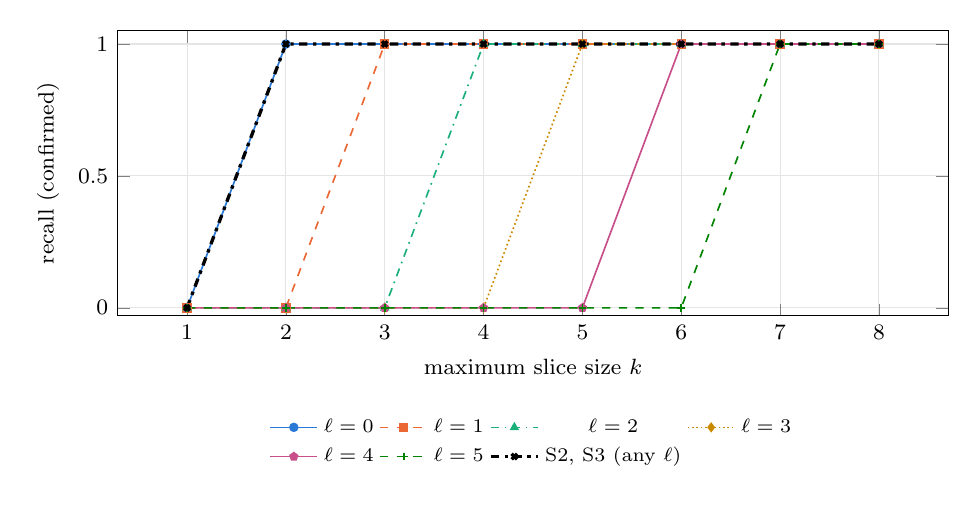
\begin{tikzpicture}\begin{axis}[width=\columnwidth,height=5.2cm,xlabel={maximum slice size $k$},ylabel={recall (confirmed)},xtick={1,2,3,4,5,6,7,8},ymin=-0.03,ymax=1.05,grid=major,grid style={gray!20},legend columns=4,legend style={at={(0.5,-0.32)},anchor=north,font=\scriptsize,draw=none,fill=none},tick label style={font=\footnotesize},label style={font=\footnotesize}]
\addplot[cA,semithick,solid,mark=*,mark size=1.4pt,mark options={solid}] coordinates {(1,0) (2,1) (3,1) (4,1) (5,1) (6,1) (7,1) (8,1)};
\addlegendentry{$\ell=0$}
\addplot[cB,semithick,dashed,mark=square*,mark size=1.4pt,mark options={solid}] coordinates {(1,0) (2,0) (3,1) (4,1) (5,1) (6,1) (7,1) (8,1)};
\addlegendentry{$\ell=1$}
\addplot[cC,semithick,dashdotted,mark=triangle*,mark size=1.4pt,mark options={solid}] coordinates {(1,0) (2,0) (3,0) (4,1) (5,1) (6,1) (7,1) (8,1)};
\addlegendentry{$\ell=2$}
\addplot[cD,semithick,densely dotted,mark=diamond*,mark size=1.4pt,mark options={solid}] coordinates {(1,0) (2,0) (3,0) (4,0) (5,1) (6,1) (7,1) (8,1)};
\addlegendentry{$\ell=3$}
\addplot[cE,semithick,solid,mark=pentagon*,mark size=1.4pt,mark options={solid}] coordinates {(1,0) (2,0) (3,0) (4,0) (5,0) (6,1) (7,1) (8,1)};
\addlegendentry{$\ell=4$}
\addplot[cF,semithick,dashed,mark=+,mark size=1.4pt,mark options={solid}] coordinates {(1,0) (2,0) (3,0) (4,0) (5,0) (6,0) (7,1) (8,1)};
\addlegendentry{$\ell=5$}
\addplot[black,very thick,dashdotted,mark=x,mark size=1.4pt,mark options={solid}] coordinates {(1,0) (2,1) (3,1) (4,1) (5,1) (6,1) (7,1) (8,1)};
\addlegendentry{S2, S3 (any $\ell$)}
\end{axis}\end{tikzpicture}}
\newcommand{\figEvolution}{%
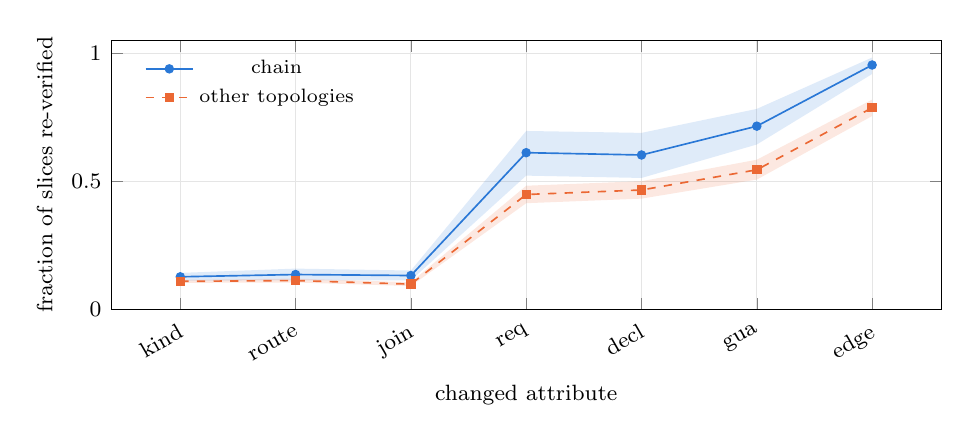
\begin{tikzpicture}\begin{axis}[width=\columnwidth,height=5cm,ymin=0,ymax=1.05,xtick={0,1,2,3,4,5,6},xticklabels={kind,route,join,req,decl,gua,edge},x tick label style={rotate=30,anchor=north east,font=\footnotesize},xlabel={changed attribute},ylabel={fraction of slices re-verified},grid=major,grid style={gray!20},legend pos=north west,legend style={font=\scriptsize,draw=none,fill=none},tick label style={font=\footnotesize},label style={font=\footnotesize}]
\addplot[fill=cA,fill opacity=0.15,draw=none,forget plot] coordinates {(0,0.112533) (1,0.113748) (2,0.113893) (3,0.522249) (4,0.513201) (5,0.643757) (6,0.918689) (6,0.983052) (5,0.782625) (4,0.689029) (3,0.696523) (2,0.152085) (1,0.159589) (0,0.142858)} -- cycle;
\addplot[cA,semithick,solid,mark=*,mark size=1.4pt,mark options={solid}] coordinates {(0,0.127657) (1,0.136491) (2,0.132616) (3,0.611777) (4,0.602782) (5,0.715277) (6,0.953787)};
\addlegendentry{chain}
\addplot[fill=cB,fill opacity=0.15,draw=none,forget plot] coordinates {(0,0.103981) (1,0.105449) (2,0.0916372) (3,0.414695) (4,0.43252) (5,0.506864) (6,0.754799) (6,0.818845) (5,0.584375) (4,0.500521) (3,0.482905) (2,0.10633) (1,0.120644) (0,0.115664)} -- cycle;
\addplot[cB,semithick,dashed,mark=square*,mark size=1.4pt,mark options={solid}] coordinates {(0,0.109813) (1,0.113022) (2,0.0989767) (3,0.448614) (4,0.466247) (5,0.545069) (6,0.78703)};
\addlegendentry{other topologies}
\end{axis}\end{tikzpicture}}
\newcommand{\figScalability}{%
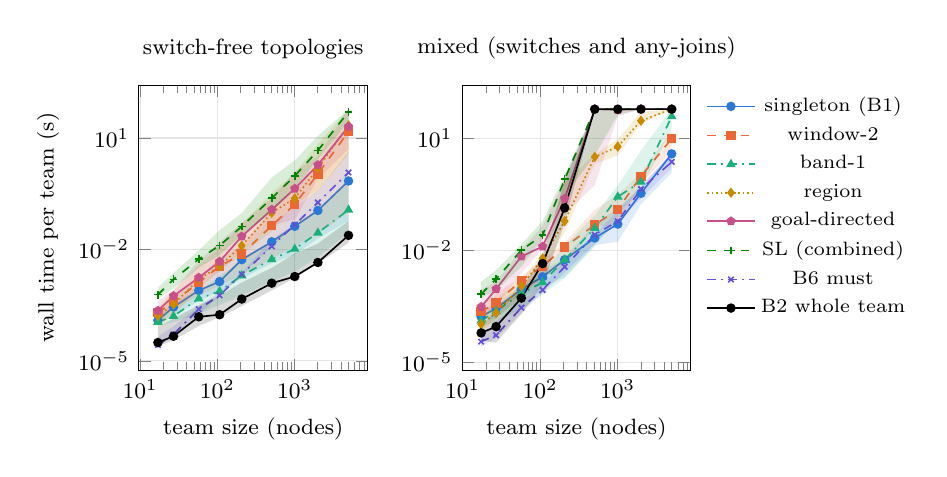
\begin{tikzpicture}
\begin{axis}[width=0.37\textwidth,height=5.2cm,xmode=log,ymode=log,xlabel={team size (nodes)},title={switch-free topologies},grid=major,grid style={gray!20},tick label style={font=\footnotesize},label style={font=\footnotesize},title style={font=\footnotesize},ylabel={wall time per team (s)},name=left]
\addplot[fill=cA,fill opacity=0.15,draw=none,forget plot] coordinates {(16.9667,0.000115132) (27.0333,0.000164556) (57.3333,0.000407352) (106.967,0.000757648) (207.033,0.00163311) (507.1,0.00427098) (1007.23,0.00721385) (2007.03,0.0197891) (5007.3,0.0596627) (5007.3,4.28992) (2007.03,0.383449) (1007.23,0.142463) (507.1,0.0469002) (207.033,0.009991) (106.967,0.00302158) (57.3333,0.000965155) (27.0333,0.000340852) (16.9667,0.000187304)} -- cycle;
\addplot[cA,semithick,solid,mark=*,mark size=1.4pt,mark options={solid}] coordinates {(16.9667,0.000123136) (27.0333,0.000281024) (57.3333,0.000786207) (106.967,0.00135545) (207.033,0.00530436) (507.1,0.0160054) (1007.23,0.0419221) (2007.03,0.11207) (5007.3,0.697767)};
\addplot[fill=cB,fill opacity=0.15,draw=none,forget plot] coordinates {(16.9667,0.00014324) (27.0333,0.000246868) (57.3333,0.000562167) (106.967,0.00106897) (207.033,0.00208542) (507.1,0.0056523) (1007.23,0.0124602) (2007.03,0.0265203) (5007.3,0.102219) (5007.3,25.2353) (2007.03,2.25582) (1007.23,0.390952) (507.1,0.115869) (207.033,0.012401) (106.967,0.0058404) (57.3333,0.00177457) (27.0333,0.000554864) (16.9667,0.000257556)} -- cycle;
\addplot[cB,semithick,dashed,mark=square*,mark size=1.4pt,mark options={solid}] coordinates {(16.9667,0.00019784) (27.0333,0.000389479) (57.3333,0.00126457) (106.967,0.00353425) (207.033,0.00743725) (507.1,0.0436425) (1007.23,0.16449) (2007.03,1.08421) (5007.3,14.9355)};
\addplot[fill=cC,fill opacity=0.15,draw=none,forget plot] coordinates {(16.9667,8.7968e-05) (27.0333,0.000109547) (57.3333,0.000184212) (106.967,0.000322715) (207.033,0.000571692) (507.1,0.00136311) (1007.23,0.00255104) (2007.03,0.00617084) (5007.3,0.0278049) (5007.3,0.621448) (2007.03,0.10475) (1007.23,0.0417048) (507.1,0.0170092) (207.033,0.00479039) (106.967,0.00189509) (57.3333,0.0007196) (27.0333,0.000251548) (16.9667,0.000148424)} -- cycle;
\addplot[cC,semithick,dashdotted,mark=triangle*,mark size=1.4pt,mark options={solid}] coordinates {(16.9667,0.000110768) (27.0333,0.0001598) (57.3333,0.000470024) (106.967,0.000745575) (207.033,0.00198543) (507.1,0.00538258) (1007.23,0.0102787) (2007.03,0.0279596) (5007.3,0.116264)};
\addplot[fill=cD,fill opacity=0.15,draw=none,forget plot] coordinates {(16.9667,7.742e-05) (27.0333,0.000174432) (57.3333,0.000855551) (106.967,0.00271361) (207.033,0.00703778) (507.1,0.0308239) (1007.23,0.165978) (2007.03,0.379865) (5007.3,3.78003) (5007.3,59.6785) (2007.03,6.88055) (1007.23,1.12619) (507.1,0.32705) (207.033,0.0476627) (106.967,0.0118282) (57.3333,0.00374626) (27.0333,0.000759007) (16.9667,0.000287892)} -- cycle;
\addplot[cD,semithick,densely dotted,mark=diamond*,mark size=1.4pt,mark options={solid}] coordinates {(16.9667,0.000160816) (27.0333,0.000330639) (57.3333,0.00156158) (106.967,0.00354511) (207.033,0.012625) (507.1,0.0971364) (1007.23,0.23807) (2007.03,1.53468) (5007.3,21.8893)};
\addplot[fill=cE,fill opacity=0.15,draw=none,forget plot] coordinates {(16.9667,0.000144036) (27.0333,0.000252324) (57.3333,0.00101828) (106.967,0.00264708) (207.033,0.0101805) (507.1,0.0445145) (1007.23,0.0639509) (2007.03,0.799506) (5007.3,5.00858) (5007.3,60) (2007.03,3.23372) (1007.23,1.27236) (507.1,0.237878) (207.033,0.0520552) (106.967,0.0157444) (57.3333,0.00492951) (27.0333,0.000803039) (16.9667,0.000411928)} -- cycle;
\addplot[cE,semithick,solid,mark=pentagon*,mark size=1.4pt,mark options={solid}] coordinates {(16.9667,0.000223887) (27.0333,0.000558112) (57.3333,0.00173792) (106.967,0.00471081) (207.033,0.0223657) (507.1,0.117656) (1007.23,0.433927) (2007.03,1.88207) (5007.3,20.2178)};
\addplot[fill=cF,fill opacity=0.15,draw=none,forget plot] coordinates {(16.9667,0.000473043) (27.0333,0.000892643) (57.3333,0.00315705) (106.967,0.00710435) (207.033,0.0241906) (507.1,0.105006) (1007.23,0.449128) (2007.03,2.66835) (5007.3,28.0007) (5007.3,60) (2007.03,11.4283) (1007.23,2.49225) (507.1,0.864475) (207.033,0.0951485) (106.967,0.0331458) (57.3333,0.00937373) (27.0333,0.00228938) (16.9667,0.000949079)} -- cycle;
\addplot[cF,semithick,dashed,mark=+,mark size=1.4pt,mark options={solid}] coordinates {(16.9667,0.000605375) (27.0333,0.0015605) (57.3333,0.00546165) (106.967,0.0128047) (207.033,0.0414717) (507.1,0.241777) (1007.23,0.955405) (2007.03,4.61001) (5007.3,51.3054)};
\addplot[fill=cG,fill opacity=0.15,draw=none,forget plot] coordinates {(16.9667,2.4116e-05) (27.0333,4.6764e-05) (57.3333,0.000177384) (106.967,0.000558308) (207.033,0.00201148) (507.1,0.0118045) (1007.23,0.0458298) (2007.03,0.181567) (5007.3,1.16079) (5007.3,1.1997) (2007.03,0.185875) (1007.23,0.0482513) (507.1,0.0188901) (207.033,0.00239557) (106.967,0.000702503) (57.3333,0.000293508) (27.0333,8.5428e-05) (16.9667,4.49717e-05)} -- cycle;
\addplot[cG,semithick,dashdotted,mark=x,mark size=1.4pt,mark options={solid}] coordinates {(16.9667,2.6472e-05) (27.0333,5.1496e-05) (57.3333,0.000245784) (106.967,0.0005782) (207.033,0.00213948) (507.1,0.0121777) (1007.23,0.0461963) (2007.03,0.183301) (5007.3,1.18172)};
\addplot[fill=black,fill opacity=0.15,draw=none,forget plot] coordinates {(16.9667,2.4608e-05) (27.0333,3.5772e-05) (57.3333,8.6644e-05) (106.967,0.000149988) (207.033,0.000298659) (507.1,0.000787587) (1007.23,0.00170126) (2007.03,0.00411229) (5007.3,0.0150857) (5007.3,0.0582666) (2007.03,0.014344) (1007.23,0.00767646) (507.1,0.00317061) (207.033,0.00127586) (106.967,0.000577555) (57.3333,0.000313668) (27.0333,0.000137391) (16.9667,8.1212e-05)} -- cycle;
\addplot[black,semithick,solid,mark=*,mark size=1.4pt,mark options={solid}] coordinates {(16.9667,3.0968e-05) (27.0333,4.592e-05) (57.3333,0.000153255) (106.967,0.000174008) (207.033,0.00046056) (507.1,0.00123265) (1007.23,0.00186136) (2007.03,0.00445267) (5007.3,0.0239017)};
\end{axis}
\begin{axis}[width=0.37\textwidth,height=5.2cm,xmode=log,ymode=log,xlabel={team size (nodes)},title={mixed (switches and any-joins)},grid=major,grid style={gray!20},tick label style={font=\footnotesize},label style={font=\footnotesize},title style={font=\footnotesize},legend pos=outer north east,legend style={font=\scriptsize,draw=none,fill=none},at={(left.east)},anchor=west,xshift=1.2cm]
\addplot[fill=cA,fill opacity=0.15,draw=none,forget plot] coordinates {(17.3,0.00012772) (27,0.000157684) (57.2,0.000525308) (107.7,0.00101981) (207.4,0.00195344) (507.2,0.0139537) (1006.7,0.0168463) (2006.8,0.171272) (5007.1,1.19564) (5007.1,4.2975) (2006.8,0.499332) (1006.7,0.133581) (507.2,0.0500044) (207.4,0.00612328) (107.7,0.00277097) (57.2,0.00117068) (27,0.000353092) (17.3,0.000218548)} -- cycle;
\addplot[cA,semithick,solid,mark=*,mark size=1.4pt,mark options={solid}] coordinates {(17.3,0.000167392) (27,0.0002812) (57.2,0.000914247) (107.7,0.00194914) (207.4,0.0056049) (507.2,0.0214753) (1006.7,0.0503732) (2006.8,0.337252) (5007.1,3.81757)};
\addlegendentry{singleton (B1)}
\addplot[fill=cB,fill opacity=0.15,draw=none,forget plot] coordinates {(17.3,0.00017516) (27,0.000240668) (57.2,0.000644183) (107.7,0.00181885) (207.4,0.00393168) (507.2,0.0424169) (1006.7,0.0453797) (2006.8,0.597342) (5007.1,4.52587) (5007.1,15.7352) (2006.8,1.16724) (1006.7,0.310516) (507.2,0.121995) (207.4,0.0159738) (107.7,0.00568093) (57.2,0.0019702) (27,0.000697019) (17.3,0.000377347)} -- cycle;
\addplot[cB,semithick,dashed,mark=square*,mark size=1.4pt,mark options={solid}] coordinates {(17.3,0.000229312) (27,0.000387359) (57.2,0.00156611) (107.7,0.00372024) (207.4,0.0121891) (507.2,0.0481263) (1006.7,0.124133) (2006.8,0.957893) (5007.1,9.77257)};
\addlegendentry{window-2}
\addplot[fill=cC,fill opacity=0.15,draw=none,forget plot] coordinates {(17.3,9.5904e-05) (27,0.000123239) (57.2,0.000267723) (107.7,0.000669491) (207.4,0.00178399) (507.2,0.0125887) (1006.7,0.0875252) (2006.8,0.44353) (5007.1,17.4452) (5007.1,60) (2006.8,4.68214) (1006.7,0.539694) (507.2,0.085952) (207.4,0.0132015) (107.7,0.00261178) (57.2,0.000836676) (27,0.000328264) (17.3,0.000175056)} -- cycle;
\addplot[cC,semithick,dashdotted,mark=triangle*,mark size=1.4pt,mark options={solid}] coordinates {(17.3,0.000130696) (27,0.000236296) (57.2,0.000700767) (107.7,0.0013889) (207.4,0.00556215) (507.2,0.0392914) (1006.7,0.271584) (2006.8,0.682607) (5007.1,38.3581)};
\addlegendentry{band-1}
\addplot[fill=cD,fill opacity=0.15,draw=none,forget plot] coordinates {(17.3,6.0804e-05) (27,0.00015262) (57.2,0.000519467) (107.7,0.00283211) (207.4,0.0308389) (507.2,2.06426) (1006.7,3.49983) (2006.8,24.1799) (5007.1,60) (5007.1,60) (2006.8,51.0248) (1006.7,9.2807) (507.2,3.70774) (207.4,0.651046) (107.7,0.00863084) (57.2,0.00157663) (27,0.00050634) (17.3,0.00017748)} -- cycle;
\addplot[cD,semithick,densely dotted,mark=diamond*,mark size=1.4pt,mark options={solid}] coordinates {(17.3,0.000105344) (27,0.000212072) (57.2,0.0010921) (107.7,0.00607017) (207.4,0.060309) (507.2,3.15748) (1006.7,5.97038) (2006.8,29.4253) (5007.1,60)};
\addlegendentry{region}
\addplot[fill=cE,fill opacity=0.15,draw=none,forget plot] coordinates {(17.3,0.000183955) (27,0.00031588) (57.2,0.00237208) (107.7,0.0115788) (207.4,0.0930357) (507.2,0.553794) (1006.7,38.8167) (2006.8,60) (5007.1,60) (5007.1,60) (2006.8,60) (1006.7,60) (507.2,60) (207.4,0.802849) (107.7,0.0449777) (57.2,0.0102977) (27,0.00144355) (17.3,0.000883519)} -- cycle;
\addplot[cE,semithick,solid,mark=pentagon*,mark size=1.4pt,mark options={solid}] coordinates {(17.3,0.000306648) (27,0.000920296) (57.2,0.00682489) (107.7,0.0126813) (207.4,0.240523) (507.2,60) (1006.7,57.2195) (2006.8,60) (5007.1,60)};
\addlegendentry{goal-directed}
\addplot[fill=cF,fill opacity=0.15,draw=none,forget plot] coordinates {(17.3,0.000540284) (27,0.000847939) (57.2,0.00364598) (107.7,0.0201406) (207.4,0.294606) (507.2,3.41308) (1006.7,41.8608) (2006.8,60) (5007.1,60) (5007.1,60) (2006.8,60) (1006.7,60) (507.2,60) (207.4,1.03491) (107.7,0.061161) (57.2,0.01423) (27,0.00296685) (17.3,0.00143343)} -- cycle;
\addplot[cF,semithick,dashed,mark=+,mark size=1.4pt,mark options={solid}] coordinates {(17.3,0.000675343) (27,0.00171201) (57.2,0.0100918) (107.7,0.0253602) (207.4,0.798198) (507.2,60) (1006.7,60) (2006.8,60) (5007.1,60)};
\addlegendentry{SL (combined)}
\addplot[fill=cG,fill opacity=0.15,draw=none,forget plot] coordinates {(17.3,2.654e-05) (27,4.546e-05) (57.2,0.000211356) (107.7,0.000733375) (207.4,0.00256424) (507.2,0.015092) (1006.7,0.0571734) (2006.8,0.245596) (5007.1,1.592) (5007.1,3.82299) (2006.8,0.532708) (1006.7,0.113077) (507.2,0.0266913) (207.4,0.00508787) (107.7,0.00118923) (57.2,0.000437723) (27,0.000126384) (17.3,4.7216e-05)} -- cycle;
\addplot[cG,semithick,dashdotted,mark=x,mark size=1.4pt,mark options={solid}] coordinates {(17.3,3.6072e-05) (27,5.3568e-05) (57.2,0.00029164) (107.7,0.000869063) (207.4,0.00362243) (507.2,0.0261982) (1006.7,0.0601835) (2006.8,0.434442) (5007.1,2.32639)};
\addlegendentry{B6 must}
\addplot[fill=black,fill opacity=0.15,draw=none,forget plot] coordinates {(17.3,3.7876e-05) (27,3.4192e-05) (57.2,0.000196772) (107.7,0.00114499) (207.4,0.0537879) (507.2,56.7204) (1006.7,60) (2006.8,60) (5007.1,60) (5007.1,60) (2006.8,60) (1006.7,60) (507.2,60) (207.4,0.76044) (107.7,0.00708778) (57.2,0.000932843) (27,0.000266623) (17.3,8.4388e-05)} -- cycle;
\addplot[black,semithick,solid,mark=*,mark size=1.4pt,mark options={solid}] coordinates {(17.3,6.1696e-05) (27,9.10875e-05) (57.2,0.000528359) (107.7,0.00441887) (207.4,0.136044) (507.2,60) (1006.7,60) (2006.8,60) (5007.1,60)};
\addlegendentry{B2 whole team}
\end{axis}
\end{tikzpicture}}
% END GENERATED RESULTS

\begin{document}

\title{Agent Slicing: Localizing Blind Spots in Declared-Contract Models of Multi-Agent AI Teams}

\author{Anonymous Authors%
\thanks{Manuscript submitted to IEEE Transactions on Software Engineering.}}

\markboth{IEEE Transactions on Software Engineering}%
{Agent Slicing: Localizing Blind Spots in Multi-Agent AI Teams}

\maketitle

\begin{abstract}
Software teams increasingly build systems in which several AI agents hand work to one another. Such a team can be unsafe even when every agent meets its own contract, because the defect lives in a relationship among agents: a join that releases on the first approval, two reviewers that share one model, a test gate whose tests were written by a fallible agent. We study this problem on \emph{declared-contract models} of agent teams: directed acyclic graphs of agents and deterministic gates with requirements, guarantees, fork, switch, join policies (all, any, quorum) and model failures. We introduce \emph{agent slicing}. A slice is a convex, possibly disconnected, set of agents analyzed exactly while the rest of the team is taken at face value. A slice reports a defect only when its witness \emph{lifts} to a run of the whole team, so reported findings are never false alarms. The size of the smallest slice that confirms a defect is its \emph{depth}; depth at least two means that checking agents one at a time cannot see it, and the smallest confirming slices localize it. We prove when slice abstraction is compositional (partitions with an acyclic quotient), that exact slice contracts are relations rather than assumption-guarantee pairs, that view-local agent checks cannot separate safe from unsafe teams on these defect classes, and that a change invalidates only a computable set of slices; we also give the complexity of each question. On \resMutTeams{} teams with naturally arising defects from random engineering changes, \resMutHiddenShare{} of the defect symptoms are hidden at agent level, and agent-level analysis finds none of them. A global must-analysis detects \resMutRecallHiddenBSix{} of them but reports \resMutFalseRateBSix{} false findings and names only the symptom node; confirmed slice analysis detects all of them with no false finding and returns an exact minimal slice for \resMutExactSL{} (\resMutShrinkExact{} when a whole-team witness is shrunk slice by slice). In encodings of nine published multi-agent designs under contracts we declared and one tolerated model failure, \resArchHiddenDocumented{} contain a defect that only multi-agent slices reveal. No language model is run; we make no claim that any model meets a contract.
\end{abstract}

\begin{IEEEkeywords}
Multi-agent systems, large language models, assume-guarantee reasoning, contracts, compositional verification, fault localization.
\end{IEEEkeywords}

% =====================================================================
\section{Introduction}
\IEEEPARstart{L}{arge} language model (LLM) agents are now composed into teams that do software work. MetaGPT assigns the roles of a software company to agents that exchange documents in a fixed order~\cite{hong2024metagpt}; ChatDev runs a chain of design, coding, review and testing phases~\cite{qian2024chatdev}; AgentCoder lets a programmer agent and a test-designer agent work in parallel and runs the tests with a script~\cite{huang2023agentcoder}; Agentless and MAGIS split issue resolution into localization, repair and validation stages~\cite{xia2025agentless,tao2024magis}. Surveys list dozens of such designs~\cite{he2025llmmas,hou2024llm4se,fan2023llmse}, and frameworks such as AutoGen make it easy to wire agents into new topologies~\cite{wu2024autogen}.

These teams are engineered artifacts, so we should be able to ask an engineering question about them before they run: \emph{is the composition justified?} If every agent does what its contract says, does the team deliver what the team promises? Current practice answers other questions. Benchmarks score the final output of runs~\cite{jimenez2024swebench,liu2024agentbench,yehudai2025survey}. Guardrails and runtime enforcement check one agent's inputs, outputs or actions~\cite{inan2023llamaguard,rebedea2023nemo,wang2026agentspec}, and security benchmarks probe one agent against injected content~\cite{debenedetti2024agentdojo,greshake2023not,ruan2024toolemu}. Failure studies collect traces and attribute a failure to an agent and a step after the fact~\cite{cemri2025why,zhang2025which}. Cemri et al.\ report that many failures of multi-agent LLM systems come from inter-agent misalignment and from verification steps that do not verify~\cite{cemri2025why}. These are properties of relationships among agents.

Consider a release gate that ships a change when either the code reviewer or the security tester approves. Each agent can meet its contract, and the gate's policy is legal, yet the team can ship code that was never security tested. Inspecting any single agent shows nothing wrong. A whole-team analysis shows that a property can be missing at the output, but not \emph{which} agents let it through.

Assume-guarantee reasoning gives the vocabulary: each component assumes something about its inputs and guarantees something about its outputs, and a composition is justified when every assumption is discharged~\cite{misra1981proofs,jones1983tentative,abadi1993composing,benveniste2018contracts}. Applied to one agent at a time, with every other agent trusted to keep its contract, the check is not path-sensitive. It credits a fact to a consumer if some upstream agent claims it, even if a join may drop that branch, and it never sees two agents fail together. Classical whole-program analyses fix part of this: we show that a must-analysis in the style of monotone data-flow frameworks~\cite{kildall1973unified,kam1977monotone}, run once per failure set, detects most such defects. But it over-approximates, so it raises false alarms, and it names only the node where the symptom appears.

\textbf{This paper.} We propose \emph{agent slicing}: analyze \emph{parts of a team} exactly and the rest at face value. A slice is a set of agents that is convex in the team graph (every path between two members stays inside); it need not be connected. Within a slice, joins, routing choices and model failures are explored exactly; outside, every component is assumed to keep its contract. Face value is an approximation in both directions, so a slice can report a defect the team does not have. We therefore \emph{confirm} each slice finding by lifting its witness to a run of the whole team. The size of the smallest slice that confirms a defect is its \emph{depth}: depth one means the defect is visible to an agent-by-agent check, depth two or more means it is hidden. The smallest confirming slices \emph{localize} the defect: they name the agents whose relationship is wrong. Fig.~\ref{fig:overview} shows the idea.

\begin{figure*}[!t]
\centering
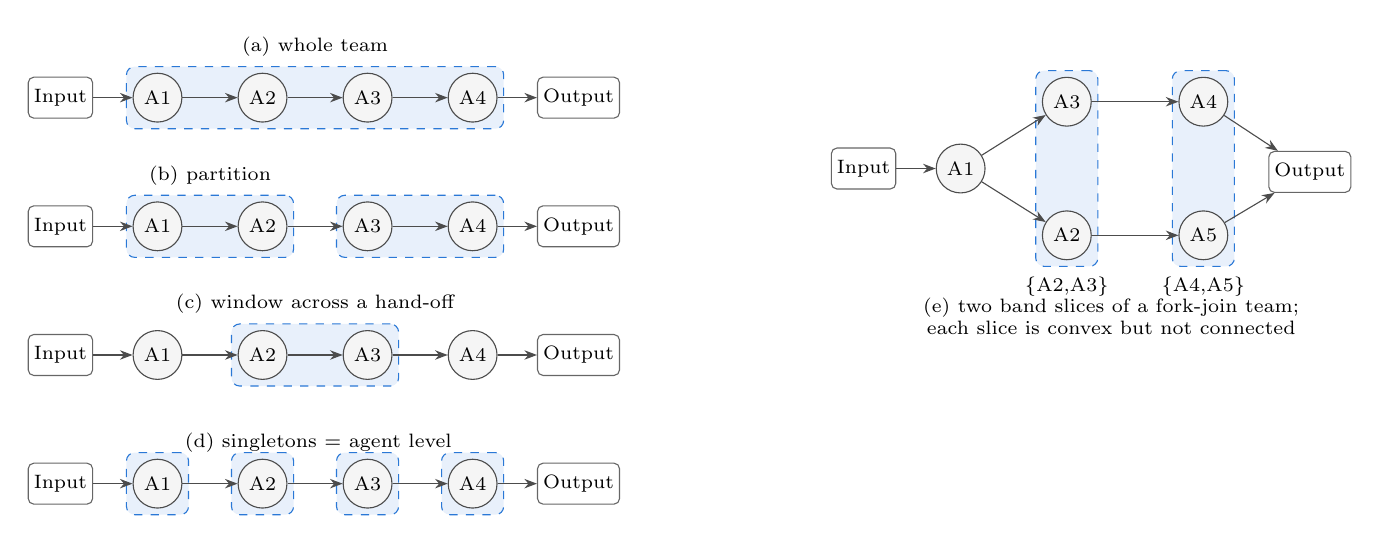
\begin{tikzpicture}[node distance=7mm]
\begin{scope}
\node[io] (i1) {Input};
\node[ag,right=5mm of i1] (a1) {A1};
\node[ag,right=of a1] (a2) {A2};
\node[ag,right=of a2] (a3) {A3};
\node[ag,right=of a3] (a4) {A4};
\node[io,right=5mm of a4] (o1) {Output};
\foreach \u/\v in {i1/a1,a1/a2,a2/a3,a3/a4,a4/o1} \draw[fl] (\u)--(\v);
\begin{scope}[on background layer]
\node[slc,fit=(a1)(a4),label={[font=\scriptsize]above:(a) whole team}] {};
\end{scope}
\node[io,below=11mm of i1] (i2) {Input};
\node[ag,right=5mm of i2] (b1) {A1};
\node[ag,right=of b1] (b2) {A2};
\node[ag,right=of b2] (b3) {A3};
\node[ag,right=of b3] (b4) {A4};
\node[io,right=5mm of b4] (o2) {Output};
\foreach \u/\v in {i2/b1,b1/b2,b2/b3,b3/b4,b4/o2} \draw[fl] (\u)--(\v);
\begin{scope}[on background layer]
\node[slc,fit=(b1)(b2),label={[font=\scriptsize]above:(b) partition}] {};
\node[slc,fit=(b3)(b4)] {};
\end{scope}
\node[io,below=11mm of i2] (i3) {Input};
\node[ag,right=5mm of i3] (c1) {A1};
\node[ag,right=of c1] (c2) {A2};
\node[ag,right=of c2] (c3) {A3};
\node[ag,right=of c3] (c4) {A4};
\node[io,right=5mm of c4] (o3) {Output};
\foreach \u/\v in {i3/c1,c1/c2,c2/c3,c3/c4,c4/o3} \draw[fl] (\u)--(\v);
\begin{scope}[on background layer]
\node[slc,fit=(c2)(c3),label={[font=\scriptsize]above:(c) window across a hand-off}] {};
\end{scope}
\node[io,below=11mm of i3] (i4) {Input};
\node[ag,right=5mm of i4] (d1) {A1};
\node[ag,right=of d1] (d2) {A2};
\node[ag,right=of d2] (d3) {A3};
\node[ag,right=of d3] (d4) {A4};
\node[io,right=5mm of d4] (o4) {Output};
\foreach \u/\v in {i4/d1,d1/d2,d2/d3,d3/d4,d4/o4} \draw[fl] (\u)--(\v);
\begin{scope}[on background layer]
\foreach \x in {d1,d2,d3,d4} \node[slc,fit=(\x)] {};
\node[font=\scriptsize,above=0.5mm of d1.north east,anchor=south west] {(d) singletons = agent level};
\end{scope}
\end{scope}
\begin{scope}[xshift=10.2cm,yshift=-0.9cm]
\node[io] (fi) {Input};
\node[ag,right=5mm of fi] (f1) {A1};
\node[ag,above right=4mm and 9mm of f1] (f3) {A3};
\node[ag,below right=4mm and 9mm of f1] (f2) {A2};
\node[ag,right=11mm of f3] (f4) {A4};
\node[ag,right=11mm of f2] (f5) {A5};
\node[io,below right=4mm and 6mm of f4] (fo) {Output};
\foreach \u/\v in {fi/f1,f1/f3,f1/f2,f3/f4,f2/f5,f4/fo,f5/fo} \draw[fl] (\u)--(\v);
\begin{scope}[on background layer]
\node[slc,fit=(f3)(f2),label={[font=\scriptsize,align=center]below:{\{A2,A3\}}}] {};
\node[slc,fit=(f4)(f5),label={[font=\scriptsize,align=center]below:{\{A4,A5\}}}] {};
\end{scope}
\node[font=\scriptsize,align=center,below=12mm of f1,anchor=north west,xshift=-6mm] {(e) two band slices of a fork-join team;\\ each slice is convex but not connected};
\end{scope}
\end{tikzpicture}
\caption{Slices of a chain (a--d) and of a fork-join team (e). A slice is a convex set of agents analyzed exactly while the rest of the team is taken at face value. Singleton slices (d) give agent-level analysis; the whole team (a) gives exact monolithic analysis. Slices in between expose and localize defects that live in hand-offs, joins and shared models.}
\label{fig:overview}
\end{figure*}

We study three research questions.

\textbf{RQ1, Formal foundation and expressiveness.} \emph{Can an agent slice be defined as a first-class contract such that slice-level reasoning is sound and compositional, recovers agent-level analysis as a special case, and is strictly more expressive than it?}

\textbf{RQ2, Detection and localization power.} \emph{How many blind spots does slice-level analysis reveal that agent-level analysis cannot, and how precisely does it localize their root causes, compared with agent-level and whole-team analysis?}

\textbf{RQ3, Cost, slicing strategy, and evolution.} \emph{What does slice-level analysis cost, how do slicing strategy and slice size trade detection power against cost and false alarms, and how much re-verification does slicing save when a team evolves?}

\textbf{Contributions.}
\begin{itemize}
\item A calculus of graph-shaped agent teams with fork, switch, join policies, conditional guarantees and model failures, with an exact semantics (Section~\ref{sec:background}).
\item \emph{Slices as analyzable components}: convex slices, a hybrid semantics whose approximation we characterize, confirmation by lifting, derived per-exit slice contracts, emergent obligations as predicates over witnesses, and slicings with an explicit acyclic-quotient condition (Section~\ref{sec:approach}).
\item The notions of \emph{depth} and \emph{minimal confirming slice}, and a taxonomy of blind spots (A1--A4, S1--S6) defined by the mechanism of their witness.
\item Results with full paper proofs: slice abstraction and partition composition (T2), soundness of confirmed findings (T3), separation from view-local agent checks (T4), localization (T5), complexity per question (T7), and incremental recertification (T8), together with two propositions (T1, T6). Per-node proof steps are SMT obligations; every theorem with a computational statement is checked against brute-force oracles on small teams.
\item An implementation, three benchmarks (injected defects, defects from random engineering changes, encodings of nine published designs), seven baselines, and a replication package that regenerates every number in the paper.
\end{itemize}

\textbf{Main results.} On teams with naturally arising defects (random engineering changes to clean teams), \resMutHiddenShare{} of the \resMutKeys{} symptoms are hidden at agent level and an agent-by-agent check finds none of them. A global must-analysis finds \resMutRecallHiddenBSix{} of the hidden ones but \resMutFalseRateBSix{} of its findings are false, and it localizes only to the symptom node. Confirmed slice analysis finds all of them with no false finding. Its explanation is an exact minimal confirming slice in \resMutExactSL{} of cases with the combined strategy, and in \resMutShrinkExact{} of cases when a whole-team witness is shrunk slice by slice (about \resMutShrinkChecks{} slice checks per defect); the deviation set of a whole-team witness, which needs no slices, is exact in \resMutDevExact{}. The depth needed to see a defect grows with the number of hand-offs between the interacting agents ($\ell+2$ for $\ell$ hand-offs) and not with team size. Small slices scale to thousands of agents; on choice-rich teams both large slices and whole-team checking hit time limits.

\textbf{Scope.} We ask whether a composition is justified \emph{given the declared contracts} of its parts. We do not claim that any LLM satisfies a contract, that our contracts describe the encoded systems faithfully, or that any deployed team became safer. No language model is run.

The rest of the paper is organized as follows. Section~\ref{sec:background} defines teams and their semantics and introduces the running example. Section~\ref{sec:approach} presents agent slicing and its theory. Section~\ref{sec:eval} answers the research questions. Section~\ref{sec:related} discusses related work, and Section~\ref{sec:conclusion} concludes. The appendices contain the proofs, the specification grammar, and additional tables.

% =====================================================================
\section{Background: Agent Teams and Their Semantics}\label{sec:background}

This section fixes a small model of agent teams. Table~\ref{tab:notation} summarizes the notation.

\begin{table}[!t]
\caption{Notation}
\label{tab:notation}
\centering
\footnotesize
\begin{tabular}{@{}lp{5.7cm}@{}}
\toprule
Symbol & Meaning\\
\midrule
$\Props$ & properties (facts about the work product)\\
$\Phi,\Phi_c$ & goals of the team; critical goals\\
$f$ & fault budget: how many models may fail in one run\\
$N,E,\iota,\omega$ & nodes, edges, input node, output node\\
$\req,\gua,\decl$ & requirements, guarantees, declared evidence of a node\\
$\orc(n)$ & the model (oracle) an agent uses\\
$\rho=(W,C,F)$ & a run: switch choices, contributor sets, failed oracles\\
$c(v),o(v)$ & content (what $v$ receives) and output of $v$ in a run\\
$\key{kind}{v}{p}$ & a symptom key: kind, node, property\\
$\Sym(T)$ & all symptoms of team $T$ (exact semantics)\\
$\sigma$ & a slice (convex node set)\\
$H_\sigma$ & hybrid semantics: $\sigma$ exact, rest at face value\\
$\Fd{\sigma}$ & raw findings of $\sigma$ (keys of $H_\sigma$)\\
$\mathcal{C}(\sigma)$ & confirmed findings of $\sigma$ (witness lifts to $T$)\\
$\depth(\kappa),\MMS(\kappa)$ & depth; minimal confirming slices of key $\kappa$\\
\bottomrule
\end{tabular}
\end{table}

\subsection{Agents, Gates and Contracts}

A team works on a shared artifact, for example a code change, and builds up facts about it: a design exists, adequate tests exist, the tests pass. We call such facts \emph{properties} and write $\Props$ for the finite set of properties a team mentions. A component \emph{requires} some properties before it can do its job, and it \emph{guarantees} others when it does its job. This is design by contract~\cite{meyer1992applying} applied to team members.

Properties are semantic claims, not artifacts. ``\p{tests}'' means that an adequate test suite exists, not that a file named \texttt{tests} was produced. When an agent's model fails, the agent may still produce an artifact, for example a weak test suite, but the property it claims does not hold. A downstream test runner that requires \p{tests} then cannot establish \p{tests\_pass}, even if it executes and reports success. So the model covers errors of commission (a wrong artifact presented as right) as well as omission, at the level of properties.

Two kinds of components matter. An \emph{agent} is driven by a language model. Its guarantee is \emph{conditional}: it holds only when the agent's requirements are met and its model (its \emph{oracle}) does not fail. A \emph{gate} is a deterministic program, such as a test runner or a schema check. A gate's guarantee is conditional on its requirements but never on a model.

An agent may also \emph{declare} evidence for itself, for example ``I read the specification''. Declared evidence counts when we decide whether that agent can act, but it never flows to other components. Semantically, declaring $p$ is the same as removing $p$ from the agent's own requirements; we keep the notion because it records a common documentation practice and makes its locality explicit.

\begin{definition}[Team]\label{def:team}
A \emph{team} is a tuple $T=(N,E,\iota,\omega,\kappa,\req,\gua,\decl,\orc,\rt,\jn)$ with goals $\Phi\subseteq\Props$, critical goals $\Phi_c\subseteq\Phi$, and a fault budget $f\in\mathbb{N}$, where:
\begin{itemize}
\item $(N,E)$ is a finite directed acyclic graph with a unique source $\iota$ (the input) and a unique sink $\omega$ (the output), and every node lies on a path from $\iota$ to $\omega$;
\item $\kappa(n)\in\{\mathsf{agent},\mathsf{gate}\}$; $\iota$ and $\omega$ are gates;
\item $\req(n),\gua(n),\decl(n)\subseteq\Props$ are the requirements, guarantees and declared evidence of $n$; $\gua(\iota)$ are the input facts, and $\req(\omega)=\Phi$;
\item $\orc(n)$ names the oracle of each agent; agents may share an oracle;
\item $\rt(n)\in\{\mathsf{fork},\mathsf{switch}\}$ says whether $n$ delivers to all successors or to exactly one;
\item $\jn(n)\in\{\mathsf{all}\}\cup\{1,\ldots,|\pred(n)|\}$ is the join policy of a node with several predecessors; \texttt{any} is the quorum $1$.
\end{itemize}
\end{definition}

We write $\pred(n)$ and $\succs(n)$ for direct predecessors and successors, and $\anc(n)$ and $\desc(n)$ for proper ancestors and descendants; $\anc^*$ and $\desc^*$ include the node itself. A switch with one successor is a fork.

\subsection{Runs}

A run resolves every choice the team leaves open: which successor a switch picks, which delivered inputs a quorum or \texttt{any} join actually uses, and which oracles fail.

\begin{definition}[Run]\label{def:run}
A \emph{run} $\rho=(W,C,F)$ chooses a successor $W(n)$ for each switch, a contributor set $C(n)$ for each node with several predecessors, and a set $F$ of failed oracles with $|F|\le f$. A run is \emph{fault-free} if $F=\emptyset$. In topological order:
\begin{enumerate}
\item $\iota$ is reached, with content $c(\iota)=\emptyset$ and output $o(\iota)=\gua(\iota)$;
\item an edge $(u,v)$ is \emph{delivered} if $u$ is reached and $u$ is a fork or $W(u)=v$; $D(v)$ is the set of delivered in-edges of $v$;
\item $v$ is reached if $D(v)$ meets its policy: all in-edges for \textsf{all} (and for a single in-edge), at least $q$ for quorum $q$; then $C(v)$ is all in-edges for \textsf{all}, and a subset of $D(v)$ with $|C(v)|\ge q$ for quorum $q$;
\item the content is $c(v)=\bigcup_{(u,v)\in C(v)} o(u)$;
\item $v$ \emph{applies} if $\req(v)\subseteq c(v)\cup\decl(v)$ and $v$ is a gate or $\orc(v)\notin F$;
\item the output is $o(v)=c(v)\cup\gua(v)$ if $v$ applies, and $o(v)=c(v)$ otherwise.
\end{enumerate}
\end{definition}

Properties flow along the contributing lineage. A join that uses one branch forgets what the other branch established; this is what makes \texttt{any} and quorum joins interesting.

\subsection{Symptoms and Safety}

A team can go wrong in three observable ways: a component acts without a property it requires, the output misses a goal, or the output misses a critical goal when up to $f$ oracles fail. We name each by a \emph{key}, a triple of kind, node and property.

\begin{definition}[Symptoms, safety]\label{def:sym}
The \emph{symptoms} $\Sym(T)$ of a team are the keys
\begin{itemize}
\item $\key{assume}{v}{p}$: some fault-free run reaches $v\neq\omega$ with $p\in\req(v)\setminus(c(v)\cup\decl(v))$;
\item $\key{goal}{\omega}{\varphi}$: some fault-free run reaches $\omega$ with $\varphi\in\Phi\setminus c(\omega)$;
\item $\key{robust}{\omega}{\varphi}$: $\key{goal}{\omega}{\varphi}\notin\Sym(T)$, and some run with $|F|\le f$ reaches $\omega$ with $\varphi\in\Phi_c\setminus c(\omega)$.
\end{itemize}
$T$ is \emph{safe} if $\Sym(T)$ contains no goal or robust key, and \emph{clean} if $\Sym(T)=\emptyset$.
\end{definition}

Two remarks on scope. Safety is a partial-correctness notion: a run in which the output is never reached (for example, an \textsf{all}-join behind a switch) produces no symptom. And under failures we check only critical goals at the output; an agent acting without its requirements because an upstream model failed is the expected consequence of the failure, not a design defect.

\subsection{From Models to Runs}

The guarantee we want is about all behaviors that respect the contracts. In such a behavior a component may know more than its content: an agent may happen to see a fact nobody guaranteed.

\begin{definition}[Contract-respecting model]\label{def:model}
A \emph{model} of $T$ is a run $(W,C,F)$ together with evidence sets $E(v)\supseteq c(v)\cup\decl(v)$ for reached nodes, where contents are computed as in Definition~\ref{def:run} except that $v$ applies if $\req(v)\subseteq E(v)$ and its oracle has not failed. Its keys are those of Definition~\ref{def:sym} with $E(v)$ in place of $c(v)\cup\decl(v)$ (and $E(\omega)$ in place of $c(\omega)$).
\end{definition}

Models differ from runs only by extra evidence. This is a modeling choice: we let a component know more than it was told, but not less. The following lemmas show that runs, and only a few of them, suffice.

\begin{lemma}[Worst case, W]\label{lem:w}
A key is produced by some model if and only if it is produced by some run.
\end{lemma}

\begin{lemma}[Minimal choices, M]\label{lem:m}
Content is monotone in the contributor sets and antitone in the failure set. To decide $\Sym(T)$ it suffices to enumerate runs whose quorum joins use exactly $q$ contributors and whose failure sets have size $\min(f,|\Orc|)$.
\end{lemma}

The idea behind Lemma~\ref{lem:w} is that more evidence can only make more components apply, which only adds properties downstream; the minimal evidence $c(v)\cup\decl(v)$ is the worst case. Proofs are in Appendix~\ref{app:proofs}.

\subsection{Running Example}\label{sec:running}

We use two small software teams throughout (Fig.~\ref{fig:running}).

\begin{figure*}[!t]
\centering
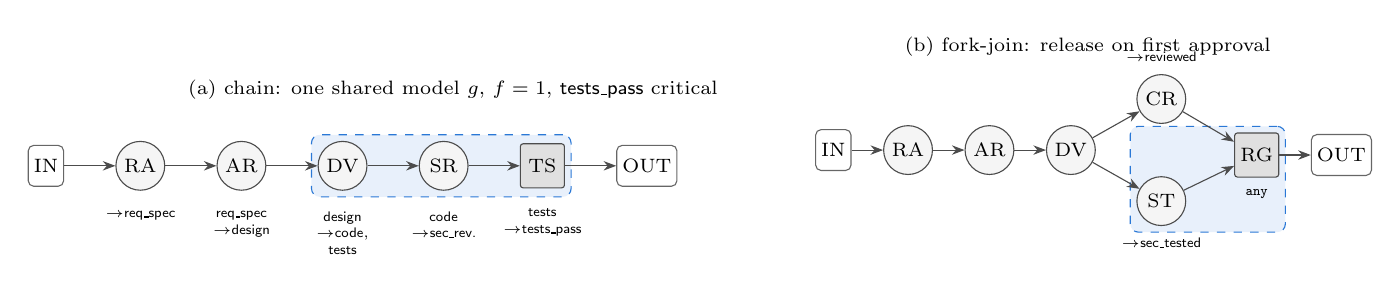
\begin{tikzpicture}[node distance=6.5mm]
\node[io] (in) {IN};
\node[ag,right=of in] (ra) {RA};
\node[ag,right=of ra] (ar) {AR};
\node[ag,right=of ar] (dv) {DV};
\node[ag,right=of dv] (sr) {SR};
\node[gt,right=of sr] (ts) {TS};
\node[io,right=of ts] (out) {OUT};
\foreach \u/\v in {in/ra,ra/ar,ar/dv,dv/sr,sr/ts,ts/out} \draw[fl] (\u)--(\v);
\begin{scope}[font=\tiny,align=center,inner sep=1pt]
\node[below=2.2mm of ra] {$\to$\p{req\_spec}};
\node[below=2.2mm of ar] {\p{req\_spec}\\$\to$\p{design}};
\node[below=2.2mm of dv] {\p{design}\\$\to$\p{code},\\\p{tests}};
\node[below=2.2mm of sr] {\p{code}\\$\to$\p{sec\_rev.}};
\node[below=2.2mm of ts] {\p{tests}\\$\to$\p{tests\_pass}};
\end{scope}
\begin{scope}[on background layer]
\node[slc,fit=(dv)(ts)] {};
\end{scope}
\node[font=\scriptsize,above=4mm of ar,anchor=south west,xshift=-8mm] {(a) chain: one shared model $g$, $f=1$, \p{tests\_pass} critical};
\begin{scope}[xshift=10.0cm,yshift=0.2cm]
\node[io] (in2) {IN};
\node[ag,right=4mm of in2] (ra2) {RA};
\node[ag,right=4mm of ra2] (ar2) {AR};
\node[ag,right=4mm of ar2] (dv2) {DV};
\node[ag,above right=2mm and 7mm of dv2] (cr2) {CR};
\node[ag,below right=2mm and 7mm of dv2] (st2) {ST};
\node[gt,below right=2mm and 7mm of cr2] (rg2) {RG};
\node[io,right=4mm of rg2] (out2) {OUT};
\foreach \u/\v in {in2/ra2,ra2/ar2,ar2/dv2,dv2/cr2,dv2/st2,cr2/rg2,st2/rg2,rg2/out2} \draw[fl] (\u)--(\v);
\node[font=\tiny,below=0.3mm of rg2] {\texttt{any}};
\node[font=\tiny,above=0.3mm of cr2] {$\to$\p{reviewed}};
\node[font=\tiny,below=0.3mm of st2] {$\to$\p{sec\_tested}};
\node[font=\scriptsize,above=7.5mm of ar2,anchor=south west,xshift=-12mm] {(b) fork-join: release on first approval};
\begin{scope}[on background layer]
\node[slc,fit=(st2)(rg2)] {};
\end{scope}
\end{scope}
\end{tikzpicture}
\caption{Running example. Circles are agents, squares are gates. Labels show requirements and ($\to$) guarantees. Agent-level analysis reports nothing for either team. Shaded: minimal confirming slices, $\{$DV, SR, TS$\}$ for the chain (a robust loss of \p{tests\_pass}) and $\{$ST, RG$\}$ (one of two) for the fork-join team.}
\label{fig:running}
\end{figure*}

\textbf{Chain.} A requirements analyst (RA) writes a specification; an architect (AR) turns it into a design; a developer (DV) writes code and tests; a security reviewer (SR) reviews the code; a deterministic test runner (TS) runs the tests and guarantees \p{tests\_pass}. The goals are \p{tests\_pass} and \p{sec\_reviewed}; \p{tests\_pass} is critical, and one model failure is tolerated ($f=1$). All four agents use the same model $g$.

Look at each component alone. AR needs \p{req\_spec}, which RA guarantees upstream. DV needs \p{design}, guaranteed by AR. SR needs \p{code} and TS needs \p{tests}, both guaranteed by DV. The critical goal is guaranteed by a \emph{gate}, so it seems not to depend on any model. Every assumption is matched; an agent-level check reports nothing. Yet the team is not robust. If model $g$ fails at DV, the tests DV writes are not adequate, TS cannot establish \p{tests\_pass}, and the release lacks its critical goal. The defect is neither in DV (it is allowed to fail; $f=1$) nor in TS (it behaves correctly). It lies in the relationship: \emph{a deterministic gate's critical guarantee rests on a fallible agent's provision.}

\textbf{Fork-join.} The analyst, architect and developer form a chain. The developer's code then forks to a code reviewer (CR), which guarantees \p{reviewed}, and a security tester (ST), which guarantees \p{sec\_tested}. Both feed a release gate (RG) with policy \texttt{any}: release on the first approval. Every requirement is matched and every goal is claimed by an ancestor of the output. Agent-level analysis is silent. But a run in which RG uses only CR's approval releases code that was not security tested, and the converse run releases code that was not reviewed.

% =====================================================================
\section{Agent Slicing}\label{sec:approach}

\subsection{Overview}

The analysis takes a team specification and a \emph{slicing strategy}. The strategy proposes slices. For each slice, the analysis explores the slice's internal behaviors exactly while taking the rest of the team at face value, and records every symptom it sees with a witness. Each witness is then \emph{lifted}: the analysis searches for a run of the whole team that agrees with the witness inside the slice and shows the same symptom. Only confirmed findings are reported, each with its smallest confirming slices, a mechanism class, and the lifted run. Safety is certified separately, either with the slice of all nodes or compositionally with a partition (Theorem~\ref{thm:abs}). As an alternative to fixed strategies, a whole-team witness can be \emph{shrunk} slice by slice until no member can be removed.

\subsection{Slices}

A slice should be a well-defined sub-computation: work that enters it should not leave it and come back. Otherwise the slice's behavior would depend on what happens outside in the middle of its own computation.

\begin{definition}[Slice]\label{def:slice}
A \emph{slice} is a nonempty set $\sigma\subseteq N$ that is \emph{convex}: for all $u,w\in\sigma$, every path from $u$ to $w$ lies in $\sigma$. Its \emph{entry edges} go from outside into $\sigma$; its \emph{exit edges} go from $\sigma$ to outside. The \emph{hull} $\hull(U)=\anc^*(U)\cap\desc^*(U)$ is the smallest convex superset of $U\subseteq N$.
\end{definition}

Connectedness is not required. In the fork-join team, $\{$CR, ST$\}$ is a slice: there is no path between the two. $\{$RA, DV$\}$ is not a slice, because the path RA$\to$AR$\to$DV leaves it; its hull is $\{$RA, AR, DV$\}$.

\begin{lemma}[Convexity]\label{lem:convex}
If $\sigma$ is convex, no node outside $\sigma$ is both an ancestor and a descendant of members. Hence outside predecessors of members have no member ancestor. Contracting $\sigma$ to one node (all other nodes kept) leaves a DAG if and only if $\sigma$ is convex.
\end{lemma}

\subsection{Hybrid Semantics}

To analyze a slice in isolation we must say what the rest of the team does. We take it at \emph{face value}: every outside component is assumed to keep its contract and to deliver everywhere.

\begin{definition}[Hybrid semantics]\label{def:hybrid}
The hybrid semantics $H_\sigma$ is defined like Definition~\ref{def:run} with these changes. Runs choose only member switches, member contributor sets, and failures $F\subseteq\orc(\sigma)$ with $|F|\le f$. Every \emph{outside} node is reached if it is $\iota$ or at least one in-edge is delivered (whatever its policy), all its delivered in-edges contribute, it always applies, and it delivers to all successors. Every entry edge into a member $v$ is delivered and carries the same environment $\env_\sigma(v)=\bigcup_{u\in\pred(v)\setminus\sigma} o(u)$, the union of the face-value outputs of all outside predecessors. The \emph{raw findings} $\Fd{\sigma}$ are the keys of Definition~\ref{def:sym} evaluated in $H_\sigma$ at every node, where a robust key requires the goal key of the same property to be absent from $\Fd{\sigma}$.
\end{definition}

By Lemma~\ref{lem:convex}, the outside predecessors of a member are never influenced by members, so $\env_\sigma(v)$ is a fixed set. Outside nodes \emph{below} members are recomputed in each run; this is how an internal failure becomes visible at the output. With $\sigma=N$ nothing is outside, $H_N$ is the exact semantics, and $\Fd{N}=\Sym(T)$. With $\sigma=\emptyset$ every node applies; $\Fd{\emptyset}$ are the requirements and goals that no ancestor claims at all (\emph{static} keys).

\begin{lemma}[Face value dominates content, A]\label{lem:face}
Let $\sigma\subseteq\sigma'$, let $\rho'$ be a run of $H_{\sigma'}$, and let $\rho$ be the run of $H_\sigma$ with the same choices on $\sigma$ and failures $F'\cap\orc(\sigma)$. Every node reached in $\rho'$ is reached in $\rho$, and its content in $\rho'$ is a subset of its content in $\rho$.
\end{lemma}

So, run by run, analyzing more components exactly can only remove content. But $H_\sigma$ also has runs with no counterpart in the team. An outside \textsf{all}-join is reached on a single input, and an outside switch delivers to both branches, so $H_\sigma$ over-approximates reachability while it under-approximates missing properties. Its raw findings are therefore neither a may- nor a must-approximation of $\Sym(T)$.

\begin{example}[A raw false alarm]\label{ex:falsealarm}
Let a switch gate $s$ route either to a gate $a$ (which guarantees $x$) or to the output, and let a gate $J$ with an \textsf{all}-join of $\iota$ and $a$ require $x$; the output joins $s$ and $J$ with \texttt{any}. In the team, $J$ is reached only when $s$ routes to $a$, and then $x$ is present: $\Sym(T)=\emptyset$. In the singleton slice $\{s\}$, $J$ is outside and reached on $\iota$'s edge alone, so $\key{assume}{J}{x}\in\Fd{\{s\}}$.
\end{example}

We therefore never report a raw finding directly.

\begin{definition}[Confirmed findings]\label{def:confirmed}
A raw finding $\kappa\in\Fd{\sigma}$ with witness $\rho_\sigma$ \emph{lifts} if some run $\rho$ of $T$ exhibits $\kappa$ (for a robust key: misses the property at $\omega$ under $|F|\le f$), and the run of $H_\sigma$ that makes $\rho$'s choices on $\sigma$, with failures $F\cap\orc(\sigma)$, exhibits $\kappa$ as well. The \emph{confirmed findings} $\mathcal{C}(\sigma)$ are the raw findings with a witness that lifts.
\end{definition}

The definition ties a finding to the slice: the team must show the symptom, \emph{and} the slice must show it for the same internal choices. The implementation searches team runs with the witness's member switch choices fixed and everything else free, and replays each candidate in $H_\sigma$; it explores all witnesses of a key, not only one, because the slice's minimal-choice enumeration (Lemma~\ref{lem:m}) may pick a representative that does not lift. In the worst case, lifting is as hard as whole-team checking (Theorem~\ref{thm:cx}); in our benchmarks a slice finding needed \resSLLifts{} lift searches on average and each took milliseconds.

\subsection{Agent-Level Analysis}

What does it mean to check a team agent by agent? The natural reading is: check each agent against its own contract, assuming every other component keeps its contract. That is the hybrid semantics of a singleton slice.

\begin{definition}[Agent-level analysis]\label{def:al}
The raw agent-level findings are $\bigcup_{v}\Fd{\{v\}}$; the (confirmed) agent-level findings are $\AL(T)=\bigcup_{v}\mathcal{C}(\{v\})$.
\end{definition}

\begin{proposition}[What agent level sees, T1]\label{prop:al}
For every node $v$, $\Fd{\emptyset}\subseteq\Fd{\{v\}}$, and the keys located at $v$ in $\Fd{\{v\}}$ are exactly the static keys at $v$. Every key in $\Fd{\{v\}}\setminus\Fd{\emptyset}$ has a witness in which $v$ does not apply (its requirements are unclaimed upstream, or its oracle fails) or $v$ is a switch.
\end{proposition}

The proposition explains the silence in the running example. A singleton slice gives every entry edge the same environment, so a join's own singleton sees the union of its inputs and never the choice it makes. One agent's failure is seen, but never two agents failing together, and a gate never sees where its inputs came from. In the chain, $\Fd{\{v\}}=\emptyset$ for every $v$: the singleton $\{$DV$\}$ can fail, but TS outside still applies at face value.

\subsection{Slice Contracts}

A slice is a component, so it should have a contract. Within a slice, a member's requirement may be established by another member, or it may have to come from outside; only the latter belong in the slice's assumptions. And the slice guarantees on an exit only what holds there on every behavior.

\begin{definition}[Derived slice contract]\label{def:contract}
For a slice $\sigma$ and an environment $X\subseteq\Props$ carried by every entry edge:
\begin{itemize}
\item the \emph{entry assumptions} $A_\sigma$ are the pairs $(v,p)$ with $v\in\sigma$ and $p\in\req(v)$ such that some fault-free internal run with empty environment reaches $v$ without $p$ in $c(v)\cup\decl(v)$;
\item the \emph{exit guarantee} $G_{\sigma,e}(X)$ of an exit edge $e$ is the intersection, over the fault-free internal runs that deliver $e$, of the output crossing $e$; $G^f_{\sigma,e}(X)$ is the same over runs with $|F|\le f$; the uniform guarantee is $G_\sigma(X)=\bigcap_e G_{\sigma,e}(X)$;
\item the \emph{naive guarantee} $N_{\sigma,e}(X)$ is what composing member contracts at face value promises on $e$: $X$ plus every guarantee of a member that is an ancestor-or-self of the exit's source.
\end{itemize}
\end{definition}

The gap between naive and derived guarantees is what a slice adds. Each confirmed finding witnesses such a gap, and its witness tells \emph{why} a claimed property did not arrive. For a key $\kappa$ about property $p$ at node $x$, with confirming witness $\rho$ on $\sigma$, each claimer $u$ of $p$ among the ancestors of $x$ is in one of four states: \emph{route} ($u$ is unreached because a switch chose another branch), \emph{drop} ($u$ applied but a join did not take its output into $x$'s lineage), \emph{cond} ($u$ did not apply because a requirement was missing), or \emph{fault} ($u$ did not apply because its oracle failed). The \emph{emergent obligations} $X_\sigma$ are the slice-level conditions that exclude these states, and the taxonomy (Table~\ref{tab:classes}) classifies findings by the state that occurs. Joint coverage excludes \emph{drop}, non-bypass excludes \emph{route}, conditional backing excludes \emph{cond} under failures, and oracle independence excludes two \emph{fault} claimers on one oracle. No single member can carry these obligations: each speaks about two or more components.

Table~\ref{tab:contracts} shows derived contracts for the running example. For $\{$DV, SR, TS$\}$ the fault-free guarantee equals the naive one, but the robust guarantee loses \p{code}, \p{tests}, \p{sec\_reviewed} and \p{tests\_pass}. For $\{$SR, TS$\}$, with \p{tests} supplied from outside, the robust guarantee keeps \p{tests\_pass}, so the slice that \emph{explains} the defect must contain DV. For $\{$ST, RG$\}$ the naive guarantee contains \p{sec\_tested} but the derived one does not: joint coverage fails at RG.

\begin{table}[!t]
\caption{Derived and Naive Exit Guarantees in the Running Example (Beyond What the Entries Carry)}
\label{tab:contracts}
\centering
\footnotesize
\begin{tabular}{@{}p{1.25cm}p{1.7cm}p{2.1cm}p{2.25cm}@{}}
\toprule
Slice & Entries carry & Naive $N_\sigma$ & Derived $G_\sigma$ / $G^f_\sigma$\\
\midrule
DV, SR, TS & \p{req\_spec}, \p{design} & \p{code}, \p{tests}, \p{sec\_rev.}, \p{tests\_pass} & $G$: same; $G^f$: nothing\\
SR, TS & $+$\p{code}, \p{tests} & \p{sec\_rev.}, \p{tests\_pass} & $G$: same; $G^f$: \p{tests\_pass}\\
ST, RG & \p{spec}, \p{design}, \p{code} & \p{sec\_tested} & $G$: nothing\\
CR, RG & same as above & \p{reviewed} & $G$: nothing\\
\bottomrule
\end{tabular}
\end{table}

\begin{definition}[Declared contract, exactness]\label{def:declared}
A \emph{declared contract} of $\sigma$ is a pair $(A^d,G^d)$. It is \emph{valid} if, when every entry carries $A^d$, every member's requirements hold in every fault-free internal run and $G^d\subseteq G_{\sigma,e}(A^d)$ for every exit $e$. A pair $(A,G)$ is \emph{exact} for exit $e$ if, for every environment $X$, $G_{\sigma,e}(X)=X\cup G$ when $A\subseteq X$ and $G_{\sigma,e}(X)=X$ otherwise.
\end{definition}

\begin{definition}[Boundary behavior]\label{def:beh}
For a slice $\sigma$ and a failure set $F$, $\Beh_\sigma$ maps each delivery pattern of the entry edges and each assignment of contents to entry edges to the set of possible outcomes: which exits are delivered, with what content, and which keys arise at members. Contents are tracked symbolically: a member's content is the union of the contents of the entry edges in its \emph{flow} plus what members add.
\end{definition}

\begin{theorem}[Slice abstraction, T2]\label{thm:abs}
\begin{enumerate}
\item[(a)] Replacing a convex slice $\sigma$ by a macro component whose behavior is $\Beh_\sigma$ (evaluated with the run's global failure set) leaves every assume and goal key of $T$ unchanged, and leaves the set of properties missing at $\omega$ under each failure set unchanged; hence $\Sym(T)$ is unchanged.
\item[(b)] Let $f=0$ and let every run of $T$ deliver either all or none of $\sigma$'s entry edges (as for single-entry slices). If $(A^d,G^d)$ is valid and the team in which $\sigma$ is replaced by a component that, when its entries carry $A^d$, delivers on any nonempty subset of its exits with content at least $A^d\cup G^d$, and otherwise delivers on any subset with any content, has no goal key, then $T$ has no goal key.
\item[(c)] An exit whose guarantee is $g$ if $r_1$ or $r_2$ enters (two members $r_1\to g$ and $r_2\to g$ feeding one exit node) has no exact single pair $(A,G)$, for any distinct $r_1,r_2,g$.
\item[(d)] Let $\{\sigma_1,\ldots,\sigma_m\}$ partition $N$ (including $\iota$ and $\omega$) into convex parts whose quotient graph is acyclic. Composing the parts' boundary behaviors in the quotient's topological order, with one global failure set per run, yields $\Sym(T)$; robust keys are decided after composition. Convex parts alone do not suffice: $\{a,d\}$ and $\{b,c\}$ with edges $a\to b$ and $c\to d$ are convex and their quotient has a cycle. With a cyclic quotient, valid flat part contracts can certify an unsafe team.
\end{enumerate}
\end{theorem}

\emph{Proof idea.} (a) and (d) hold because a part's outcomes are a function of what crosses its entries and of the global failure set, and the symbolic flow makes the summary independent of the concrete entry contents. Failure sets must be global because one oracle can serve several parts; this is exactly what makes shared-model defects (S4) visible to composition. Robust keys depend on the absence of a goal key anywhere, so they are decided after composition. (b) follows from (a) because the declared component over-approximates $\Beh_\sigma$ under the stated delivery condition. (c) is the SMT obligation C2 (Table~\ref{tab:proofs}), stated over an uninterpreted sort of properties: exactness on the three environments $\emptyset$, $\{r_1\}$ and $\{r_2\}$ is already contradictory. For the cyclic example add $\iota\to a$, $\iota\to c$, $b\to\omega$, $d\to\omega$ and goals $\{x,y\}$; let $a$ and $d$ require $y$ and guarantee $x$, and $b$ and $c$ require $x$ and guarantee $y$. The part contracts ``$\{a,d\}$: assume $y$, guarantee $x$'' and ``$\{b,c\}$: assume $x$, guarantee $y$'' are valid and discharge each other, but neither $x$ nor $y$ is ever established and the output misses both goals.

\subsection{Checking Slices and Soundness}

Algorithm~\ref{alg:check} is the slice-level checker. For each slice it enumerates the minimal internal runs (Lemma~\ref{lem:m}) by depth-first search over member choices, propagates each run's effect to outside descendants (stopping where content equals face-value content), collects every distinct witness per key, and confirms keys by lifting. Findings of all slices are merged by key (Proposition~\ref{prop:overlap}), and each key is localized to its inclusion-minimal confirming slices.

\begin{algorithm}[!t]
\caption{Confirmed slice-level checking and localization}\label{alg:check}
\begin{algorithmic}[1]
\REQUIRE team $T$, family of slices $\mathcal{S}$, run budget $B$
\STATE $M \leftarrow$ empty map from keys to (slice, witness) pairs
\FORALL{static keys $\kappa\in\Fd{\emptyset}$}
  \STATE \textbf{if} some run of $T$ reaches $\kappa$'s node \textbf{then} $M[\kappa]\leftarrow\{(\bot,\cdot)\}$
\ENDFOR
\FORALL{$\sigma\in\mathcal{S}$}
  \FORALL{$F\in\{\emptyset\}\cup\{F\subseteq\orc(\sigma):|F|=\min(f,|\orc(\sigma)|)\}$}
    \FORALL{minimal internal run $\rho$ of $\sigma$ with failures $F$ (DFS; abort after $B$)}
       \STATE evaluate members; propagate to outside descendants
       \STATE record each key of $H_\sigma$ with witness $\rho$
    \ENDFOR
  \ENDFOR
  \FORALL{recorded keys $\kappa$ (not static)}
    \STATE \textbf{if} some witness of $\kappa$ lifts (Def.~\ref{def:confirmed}) \textbf{then} add $(\sigma,\rho)$ to $M[\kappa]$
  \ENDFOR
\ENDFOR
\FORALL{keys $\kappa$ in $M$}
  \STATE $\MMS(\kappa)\leftarrow$ inclusion-minimal slices in $M[\kappa]$, ranked by size, then by number of choice points
  \STATE classify $\kappa$ by the claimer states of its witness (Table~\ref{tab:classes})
\ENDFOR
\RETURN $M$, $\MMS$, classes
\end{algorithmic}
\end{algorithm}

\begin{theorem}[Soundness, T3]\label{thm:sound}
\begin{enumerate}
\item[(a)] If the family contains $N$, or if certification composes a partition with an acyclic quotient (Theorem~\ref{thm:abs}d), the verdict ``safe'' implies that $T$ is safe, and each counterexample is a run of $T$.
\item[(b)] Every confirmed finding is a symptom of $T$: $\kappa\in\mathcal{C}(\sigma)$ implies $\kappa\in\Sym(T)$, or, for a robust key, that $T$ loses the property at $\omega$ under at most $f$ failures (and $\Sym(T)$ then contains the robust key or the stronger goal key).
\item[(c)] Raw findings can be false alarms (Example~\ref{ex:falsealarm}).
\end{enumerate}
\end{theorem}

\subsection{A Taxonomy of Blind Spots}

Table~\ref{tab:classes} lists the blind-spot classes. Each is defined by the claimer states in a confirming witness (previous subsection), so the class of a finding is computed, not guessed. The first five classes are visible at agent level; S2--S6 involve a relationship among components.

\begin{table}[!t]
\caption{Blind-Spot Classes, Defined by the Claimer States of a Confirming Witness. ``AL'': Visible to Agent-Level Analysis}
\label{tab:classes}
\centering
\footnotesize
\begin{tabular}{@{}lp{5.3cm}l@{}}
\toprule
Class & Mechanism (witness states) & AL\\
\midrule
A1 & unowned goal: no component claims a goal (static) & yes\\
A2 & missing provider: a requirement no ancestor claims (static) & yes\\
A3 & ordering: the only claimer is not an ancestor of the consumer (static) & yes\\
A4 & single point of failure: the one fallible claimer of a critical goal is in state \emph{fault} & yes\\
S1 & interface gap: provided in a different view (\p{spec@raw} vs.\ \p{spec@summary}) & yes\\
S2 & joint-coverage gap: goal claimers in state \emph{drop} at an \texttt{any}/quorum join & no\\
S3 & path-merge dilution: as S2 for a fact consumed after the join & no\\
S4 & correlated evidence: two or more claimers of a critical goal in state \emph{fault} on one oracle & no\\
S5 & bypass: a claimer in state \emph{route} (a switch routes around it) & at switch\\
S6a & conditional collapse: a gate's critical claim in state \emph{cond} because an agent provision is in state \emph{fault} & no\\
S6b & conditional chain: a goal claimer in state \emph{cond} because a root assumption fails; the root is visible, the lost goal is not & no\\
\bottomrule
\end{tabular}
\end{table}

S5 is visible at the switch: the switch's singleton slice explores its choice, so its depth is one. S6b shows that ``visible'' is not ``explained'': agent-level analysis reports the unmet root assumption but never the goal lost several hand-offs later.

\subsection{Depth and Localization}

\begin{definition}[Depth, minimal confirming slices]\label{def:depth}
A slice $\sigma$ \emph{confirms} a key $\kappa$ if $\kappa\in\mathcal{C}(\sigma)$. A confirmed static key has depth $1$ and is localized at its node. Otherwise the \emph{depth} of $\kappa$ is the minimum size of a confirming slice, and $\MMS(\kappa)$ is the set of inclusion-minimal confirming slices. A symptom is \emph{hidden at agent level} if its depth is at least $2$.
\end{definition}

Depth and minimal slices are semantic: they are defined over confirmed findings, so a slice whose face-value world shows a symptom the team does not have, or shows a true symptom for a reason the team does not have, does not count. In the running example, the chain's robust loss of \p{tests\_pass} has depth \resRexChainDepth{} with the unique minimal slice $\{$DV, SR, TS$\}$; SR is included because a slice must be convex. Each goal loss of the fork-join team has depth \resRexFjDepth{} with \resRexFjMinimal{} minimal slices, $\{$CR, RG$\}$ and $\{$ST, RG$\}$: the join together with the branch it may take alone.

\begin{theorem}[Separation, T4]\label{thm:sep}
\begin{enumerate}
\item[(a)] For each class S2, S3, S4, S6a and S6b there is a family of teams, parametric in the number $\ell\ge 0$ of hand-offs between the interacting components (and, for S2 and S3, in the number $m\ge 2$ of branches), in which $\AL(T)$ contains no key of the defect (for S6b: not the goal key), the team is unsafe or unclean, and the defect has depth exactly $2$ (S2, S3) or exactly $\ell+2$ (S4, S6a, S6b).
\item[(b)] Let a \emph{view} of node $v$ be its contract, kind, oracle, policies and the set of properties claimed by its ancestors. Call an analysis \emph{view-disjunctive} if it flags a team if and only if some node's view satisfies a fixed predicate. For S2, S4 and S6a there are safe teams whose views together contain every view of an unsafe team; so no view-disjunctive analysis is both sound and free of false alarms on these classes.
\item[(c)] Recovery: every confirmed agent-level assume or goal finding is confirmed by every slice that contains its singleton, and every static key at a node $v$ is a raw finding of every slice in which $v$ is reached in some run.
\end{enumerate}
\end{theorem}

Part (b) is a limit on agent-local methods, but only on those that decide one node at a time. An analysis that combines views, such as a check that two claimers share an oracle, escapes it; so does a global must-analysis, which propagates facts along paths. We compare against both in Section~\ref{sec:eval}. Part (c) follows from the monotonicity of confirmed findings (Theorem~\ref{thm:loc}c). It does not hold for raw findings: a raw agent-level finding can disappear in a larger slice, because the larger slice shows that the singleton's witness was impossible. Together, (a) and (c) make confirmed slice-level analysis strictly more expressive than confirmed agent-level analysis.

\begin{theorem}[Localization, T5]\label{thm:loc}
\begin{enumerate}
\item[(a)] If $\kappa\in\Sym(T)$ then $\MMS(\kappa)\neq\emptyset$; in particular $N$ confirms $\kappa$.
\item[(b)] $\MMS(\kappa)$ need not be a single slice. It is a single slice if and only if the intersection of the minimal confirming slices is nonempty and confirms $\kappa$.
\item[(c)] Confirmed findings are monotone: if $\sigma\subseteq\sigma'$ are slices and $\kappa\in\mathcal{C}(\sigma)$ is an assume or goal key, then $\kappa\in\mathcal{C}(\sigma')$; for a robust key, $\kappa\in\mathcal{C}(\sigma')$ or the goal key of the same property is a raw finding of $\sigma'$. Hence the confirming slices of a key are closed upward, and $\depth(\kappa)\le k$ iff some slice of size at most $k$ confirms $\kappa$.
\item[(d)] Raw findings are not monotone: there are teams and slices $\sigma\subset\sigma'$ with $\kappa\in\Fd{\sigma}\setminus\Fd{\sigma'}$.
\end{enumerate}
\end{theorem}

For (d), let a switch $s$ route either to a gate $x$ or to the output, let $x$ join $s$ and a provider $y$ of the goal $g$ with \texttt{any}, and let the output join $s$ and $x$ with \textsf{all}. The team is clean. In $\sigma=\{s,x,y\}$ the output is outside and reached on one input; the run in which $s$ routes to $x$ and $x$ uses only $s$'s input misses $g$. In $\sigma\cup\{\omega\}$ that run no longer reaches the output. Larger slices therefore remove raw false alarms as well as reveal deeper defects; confirmation makes the picture monotone.

\begin{proposition}[Overlap, T6]\label{prop:overlap}
Keys do not depend on the slice that produced them, so findings of overlapping slices merge by key without double counting; a slice only reports the presence of keys, so findings of different slices cannot contradict each other. The family of all convex slices of size at most $k$ confirms every key of depth at most $k$.
\end{proposition}

\subsection{Slicing Strategies}

\begin{definition}[Slicing]\label{def:slicing}
A \emph{slicing} is a family of slices. A \emph{partition slicing} partitions $N$ into slices whose quotient graph is acyclic. A \emph{covering slicing} is any family; its slices may overlap.
\end{definition}

We compare these strategies. \emph{Singleton} is agent level. \emph{Whole} is the slice $N$. \emph{Window-$k$} takes, for each node, the hull of the node and its descendants within $k-1$ hops; on a chain these are the intervals of length $k$ (Fig.~\ref{fig:overview}c). \emph{Band-$w$} takes the hull of $w$ consecutive longest-path levels, a cross-section of parallel branches (Fig.~\ref{fig:overview}e). \emph{Region} takes single-entry single-exit regions: each fork or switch with its immediate post-dominator, each join with its immediate dominator, and each join with its direct predecessors~\cite{johnson1994program,lengauer1979fast}. \emph{Goal-directed} is the analogue of a backward slice~\cite{weiser1984program}: for each requirement $(v,p)$, the hull of $v$, the ancestors that claim $p$, and the ancestors that claim those claimers' requirements. \emph{Exhaustive-$k$} takes every convex slice of size at most $k$. \emph{SL} is singleton $\cup$ window-2 $\cup$ region $\cup$ goal-directed. \emph{Shrink} starts from the whole team (or a whole-team witness) and greedily removes one member at a time while the slice stays convex and still confirms the key, which yields a slice that is minimal under single removals. The analogy with program slicing is loose: only goal-directed slices have a slicing criterion, and we prove no projection property for them.

\subsection{Complexity}

\begin{theorem}[Complexity, T7]\label{thm:cx}
\begin{enumerate}
\item[(a)] Deciding whether an assume or goal key is in $\Sym(T)$ is NP-complete, already for teams of gates only, without forks, and with $f=0$. Deciding whether a robust key is in $\Sym(T)$ is in $\mathrm{D}^p$ and both NP-hard and coNP-hard. Deciding safety is coNP-complete. Deciding whether a node is reached in some run is NP-complete.
\item[(b)] Computing $\Fd{\sigma}$ takes $O(R_\sigma\cdot(|N|+|E|)\cdot\lceil|\Props|/w\rceil + R'_\sigma)$ time, where $R_\sigma$ is the number of minimal internal runs, $w$ the machine word size, and $R'_\sigma$ the (quadratic) cost of filtering minimal contributor sets. $R_\sigma$ is bounded by the product of member switch fan-outs, binomial coefficients of member quorum joins, and $1+\binom{|\orc(\sigma)|}{f}$, so it is polynomial when the member choice points and $f$ are bounded. Confirming a finding can cost as much as whole-team checking.
\item[(c)] A team can have $2^{\Theta(|N|)}$ convex slices; all convex slices of size at most $k$ are enumerated with $O(|N|^k)$ hull tests.
\item[(d)] Singleton, window, band and region strategies produce $O(|N|)$ slices, computable in $O(|N|(|N|+|E|))$ total time; goal-directed produces at most $\sum_v|\req(v)|$ slices.
\end{enumerate}
\end{theorem}

The hardness of assume and goal keys uses a CNF encoding: one switch per variable chooses a branch that provides $t_i$ or $f_i$, the branches merge with \texttt{any}, and one gate per clause requires the facts that falsify all its literals and guarantees \p{bad}~\cite{cook1971complexity}. The output requires \p{bad}, so a run misses it exactly when the formula is satisfiable. For robust keys, add an agent providing a token after the variable gadgets and make every clause gate require the token and guarantee a critical goal $c$; failing the agent's oracle always loses $c$, and fault-free runs lose $c$ iff the formula is satisfiable, so the robust key is present iff the formula is unsatisfiable. Hence robust-key membership is not in NP unless NP $=$ coNP. Safety stays coNP-complete because ``some goal or robust key exists'' is equivalent to ``some fault-free run misses a goal or some run with at most $f$ failures misses a critical goal''. Because reachability is NP-hard, Definition~\ref{def:team} requires only that every node lies on an input-output path; a node that no run reaches produces no confirmed finding.

\subsection{Incremental Recertification}

Teams change: a prompt is rewritten, a model is swapped, a join policy is relaxed. Slices make re-verification local.

\begin{theorem}[Incremental recertification, T8]\label{thm:inc}
Let a change modify node $a$, and let $\Delta$ be the symmetric difference of $a$'s old and new guarantees. The dynamic raw findings $\Fd{\sigma}\setminus\Fd{\emptyset}$ of a slice $\sigma$ that is convex in both versions are unchanged unless $\sigma$ intersects $\mathit{Dep}$, where
\begin{itemize}
\item $\mathit{Dep}=\{a\}$ for a change of oracle, kind, routing or join policy;
\item $\mathit{Dep}=\anc^*(a)$ for a change of $\req(a)$ or $\decl(a)$;
\item $\mathit{Dep}=\anc^*(Y)$ with $Y=\{a\}\cup\{y\in\desc(a):\req(y)\cap\Delta\neq\emptyset\}$ for a change of $\gua(a)$.
\end{itemize}
For an edge change $(u,v)$, let $\Delta$ be $u$'s face-value output in either version, and $Y$ be $\{u,v\}$ plus the descendants of $v$ in either version that require a property of $\Delta$; then $\mathit{Dep}$ is $\anc^*(Y)$ taken in both versions. Static findings are recomputed in linear time; slices that lose convexity, and slices that a strategy newly generates, are evaluated from scratch. The theorem concerns raw findings; confirmation depends on the whole team, so stored findings are re-confirmed after each change (one lift search per finding).
\end{theorem}

\emph{Proof idea.} An outside node is taken at face value, so its oracle, kind, routing and policy are invisible to $H_\sigma$. A requirement matters only at its node, which affects $\sigma$'s dynamic findings only if the node is a member or lies below one. A guarantee change alters contents only in the bits of $\Delta$, and those bits matter only at nodes that require them (the output requires the goals).

% =====================================================================
\section{Evaluation}\label{sec:eval}

\subsection{Implementation}

The library \texttt{slicing} (Python) implements the team model with property sets as bit masks, the exact and hybrid semantics, lifting and confirmation, slice enumeration and the strategies, derived and declared contracts, partition summaries (Theorem~\ref{thm:abs}d), the checkers and baselines, the classification of findings, incremental recertification, a topology generator, a defect injector, and a mutation operator set. Teams are written in a small JSON specification language (Appendix~\ref{app:grammar}). Three oracles serve as independent ground truth for conformance testing. The \emph{model oracle} enumerates contract-respecting models (Definition~\ref{def:model}) with all switch choices, all admissible contributor sets, all failure sets with $|F|\le f$, and every evidence assignment between the realized minimum and that minimum plus the requirements and goals of the node (the only properties evidence can affect). The \emph{replay oracle} enumerates all runs of $H_\sigma$ and replays each with an evaluator that shares no code with the checker's enumerator. The \emph{run oracle} enumerates every run of $T$ and decides confirmed findings directly from Definition~\ref{def:confirmed}, without the lifting search. Proof obligations use Z3~\cite{demoura2008z3} version \resZThreeVersion{}.

\subsection{Experimental Setup}\label{sec:setup}

An experiment plan with hypotheses, metrics, tests and decision rules was written before the first experiment and is in the replication package, with a deviation log. The plan was not registered with an external service, so its timing cannot be verified independently. The revision after the first review round changed the method (confirmation), added baselines and benchmarks, and replaced some analyses; all changes are logged and summarized in Section~\ref{sec:threats}.

\textbf{Benchmarks.} We use three.
\emph{(i) Mutation benchmark (E8).} The generator builds clean teams in seven topologies: chain, tree, fork-join, layered DAG, series-parallel, random DAG, and \emph{mixed} (series-parallel with switches and \texttt{any}-joins). It assigns contracts in topological order, drawing each requirement from a sound lower bound on the node's content, so teams are clean by construction (the exact semantics confirms this). One goal is critical and $f=1$. Each team then receives one to three random engineering changes: relax a join from \textsf{all} to a quorum, let two agents share a model, drop a guarantee, turn a gate into an agent, add a requirement, turn a fork into a switch, or remove an edge. Whatever symptoms result are the ground truth, computed with the exact semantics and cross-checked with the replay oracle on teams of up to 12 nodes. Neither the class nor the depth of a defect is chosen by us. We build \resMutTeams{} teams (7 topologies, 6 and 10 inner nodes, 20 seeds, 1--3 changes).
\emph{(ii) Injected benchmark (E2).} The injector adds exactly one defect of a chosen class to a clean team, as a small gadget with fresh property names, and records the class, the root-cause nodes and the symptom keys (verified with the exact semantics). It also builds \emph{clean} teams and four \emph{decoys}: structures that look suspicious but are safe (an \texttt{any}-join whose branches claim all goals; shared-model reviewers backed by a gate; a switch whose both branches provide the fact; a fallible provider backed by an independent gate). For each of 7 topologies, 2 host sizes, 10 seeds and 16 classes we build one team, in a \emph{small} benchmark (\resBenchNodesSmallMin--\resBenchNodesSmallMax{} nodes) and a \emph{medium} one (\resBenchNodesMediumMin--\resBenchNodesMediumMax{} nodes). Because each gadget is fixed per class and cannot interact with its host, this benchmark tests per-class behavior; its class mix, not nature, decides prevalence, and we report no prevalence from it.
\emph{(iii) Published designs (E3)}, encoded with a written protocol (Section~\ref{sec:rq2}).

\textbf{Ground truth for depth and localization.} On teams of at most 16 nodes we enumerate every convex slice of size at most 6, otherwise at most 5, and compute confirmed findings; the inclusion-minimal confirming slices of a key are its true minimal slices. This uses the same hybrid semantics as the checkers, but confirmation is checked against the independent run oracle (Section~\ref{sec:rq1}).

\textbf{Checkers.} \emph{B1} is agent-level analysis (confirmed singleton slices); \emph{B1-raw} omits confirmation. \emph{SL} and the single strategies are confirmed slice families; \emph{SL-raw} omits confirmation. \emph{B2} is the exact whole-team checker, which returns a verdict and one witness per key. We localize its findings in three ways: the hull of the witness's contributing lineage (which, as a reviewer observed, always contains the input and is therefore the symptom node's whole ancestor cone); the \emph{deviation set} of the witness (failed agents, agents that did not apply, switches, and quorum joins that used fewer inputs than they received, together with the symptom node), which needs no slices; and \emph{B2+shrink}, which shrinks the whole team slice by slice (Section~\ref{sec:approach}). \emph{B3} draws random convex slices matched to SL in number and size. \emph{B4} is a structural lint (coverage by set difference over all claims, ignoring paths). \emph{B5} is a pattern-based smell detector that flags the shapes of S2--S6 without semantics. \emph{B6} is a global must-analysis: a Kildall-style lower bound on content with union at \textsf{all}-joins and intersection at \texttt{any}/quorum joins, run once without failures and once per failure set of size $\min(f,|\Orc|)$, which reports a key wherever the lower bound lacks a required property. It is path-insensitive and linear per failure set; it localizes to the symptom node.

\textbf{Metrics.} A checker \emph{detects} a key if it reports it. On the injected benchmark the pre-registered metric is ``reports any ground-truth key''; we also report the defect's primary key (for S6b the lost goal rather than the unmet root assumption), which is what separates the classes. A reported key is \emph{false} if it is not a symptom (a robust key also counts as correct when the team loses the property without failures). Localization uses the top-ranked slice of a key: it is \emph{exact} if it is one of the true inclusion-minimal confirming slices, \emph{minimum} if its size equals the depth, and \emph{precise} if it lies within the hull of the injected root cause. The \emph{size ratio} is its size over $|N|$; \emph{cost} counts slice checks.

\textbf{Statistics.} Where outcomes are deterministic per class (0\% or 100\% on every seed), we report exact counts and one-sided 95\% Clopper--Pearson bounds instead of tests. For localization we compare per-unit exact rates (unit: topology $\times$ seed) with one-sided Wilcoxon signed-rank tests~\cite{wilcoxon1945individual}, Holm correction~\cite{holm1979simple} and Vargha--Delaney $\hat A_{12}$~\cite{vargha2000critique}, and give 95\% cluster-bootstrap intervals~\cite{efron1993introduction} that resample hosts (topology, size, seed), because each host is reused across classes and checkers~\cite{arcuri2011practical}.

\textbf{Environment.} All experiments run on one machine (20 CPU cores, Linux, Python 3.12, NumPy, SciPy, Z3), with seeds fixed in the scripts. Each result file records the commit, library versions and wall time. One command regenerates all results, tables, figures and every number in this paper.

\subsection{RQ1: Formal Foundation and Expressiveness}\label{sec:rq1}

\textbf{Method.} We validate the theory in three ways. (i) SMT obligations. The per-node steps of the proofs are formulas over arrays from an uninterpreted sort of properties to Booleans, so each holds for every property universe and every contract; an obligation is valid if its negation is unsatisfiable. These are one-step set identities; they guard the definitions against slips, not the inductions over topological order, which are proved on paper. Six \emph{proof mutants} each change one definition (for example, letting declared evidence flow on) and must break the obligation that depends on it. (ii) Conformance. On \resWildTeams{} random ``wild'' teams with arbitrary contracts, policies, switches and faults (3--7 inner nodes) and on \resBenchTeams{} small injected teams (4--7 inner nodes before injection), we compare the implementation with the three oracles and check each computational theorem statement directly, for all convex slices of size at most 3 (2 for the run oracle). (iii) The hardness reductions of Theorem~\ref{thm:cx} on \resReductionFormulas{} random 3-CNF formulas, and the view-disjunctive constructions of Theorem~\ref{thm:sep}b.

\begin{table}[!t]
\caption{SMT Proof Obligations (Z3 \resZThreeVersion). ``Valid'': the Negation Is Unsatisfiable; ``Countermodel'': a Satisfying Model Exists, as Intended}
\label{tab:proofs}
\centering
\footnotesize
\begin{tabular}{@{}llp{1.5cm}ll@{}}
\toprule
ID & Obligation & Used in & Kind & OK\\
\midrule
\tabProofs
\bottomrule
\end{tabular}
\end{table}

\begin{table}[!t]
\caption{Conformance Against Brute-Force Oracles: Teams Checked (Wild, Injected) and Teams With Any Mismatch}
\label{tab:conformance}
\centering
\footnotesize
\begin{tabular}{@{}p{4.3cm}rrr@{}}
\toprule
Check & Wild & Inj. & Mism.\\
\midrule
\tabConformance
\bottomrule
\end{tabular}
\end{table}

\textbf{Results.} All \resProofObligations{} obligations behave as expected (\resProofSteps{} valid steps and \resProofCountermodels{} intended countermodel; Table~\ref{tab:proofs}); the countermodel shows that the conditional transfer does not distribute over intersection, which is why a must-analysis cannot be exact. All \resMutantsKilled{} of \resMutants{} mutants are killed. Table~\ref{tab:conformance} shows \resConformanceMismatches{} mismatching teams in \resConformanceComparisons{} team-check pairs, including confirmed findings against the run oracle, the monotonicity of confirmed findings, partition composition, and incremental recertification after node and edge changes. The model oracle agrees with the run semantics on \resModelOracleTeams{} teams. The reductions agree with a SAT solver on all formulas (\resReductionDisagreements{} disagreements for goal keys, \resReductionRobustDisagreements{} for robust keys, which are present exactly when the formula is unsatisfiable), and the view-disjunctive constructions behave as Theorem~\ref{thm:sep}b states (\resFoolingAllHold{} conditions hold). These checks cover small teams only; they are evidence, not proof, for larger teams.

Conformance testing found two real bugs, both logged in the replication package. A switch with one successor was treated as choosing nothing; every evaluator read the same field the same way, so the oracles agreed with the checker until a theorem check exposed it. And the first version of lifting fixed the witness's contributor sets, which missed liftable witnesses that differ only in which entry edge or which non-minimal contributor set they use; the run oracle exposed it. Oracles that share a data model can share a misreading of it; we return to this in Section~\ref{sec:threats}.

\answer{RQ1}{Yes, with qualifications. A slice is a convex set of agents with a hybrid semantics, per-exit derived contracts and emergent obligations defined over witnesses. Raw slice findings are approximations in both directions; confirmed findings are sound (T3b) and monotone in the slice (T5c). The singleton slicing is agent-level analysis, every confirmed agent-level finding is recovered by larger slices, and some defect families are invisible to it (T4a), so confirmed slice-level analysis is strictly more expressive. View-disjunctive agent checks cannot separate safe from unsafe teams on S2, S4 and S6a (T4b). Slice abstraction is compositional over partitions with an acyclic quotient and a global failure set (T2d); exact contracts are relations, not pairs (T2c). Per-node steps are SMT-checked; proofs of the inductions are on paper; \resConformanceComparisons{} oracle comparisons on small teams show no mismatch.}

\subsection{RQ2: Detection and Localization Power}\label{sec:rq2}

\subsubsection{Defects from engineering changes (E8)}

Of the \resMutTeams{} mutated teams, \resMutUnclean{} have at least one symptom and \resMutUnsafe{} are unsafe; together they have \resMutKeys{} symptom keys. The replay oracle agrees with the exact semantics on all \resMutOracleTeams{} teams it checked (\resMutOracleDisagree{} disagreements).

\textbf{How often are defects hidden?} Most symptoms are visible to an agent-by-agent check: \resMutDepthOne{} keys have depth~1. But \resMutHiddenKeys{} keys (\resMutHiddenShare) have depth at least two: \resMutDepthTwo{} of depth 2, \resMutDepthThree{} of depth 3, \resMutDepthFour{} of depth 4, \resMutDepthFive{} of depth 5 and \resMutDepthSix{} of depth 6. \resMutTeamsWithHidden{} teams have at least one hidden key, and in \resMutTeamsHiddenOnly{} teams every symptom is hidden, so an agent-level check would report the team as clean. Table~\ref{tab:mutop} shows which changes produce hidden defects: relaxing a join is the most dangerous change, followed by letting two agents share a model.

\begin{table}[!t]
\caption{Mutation Benchmark: Detection (\% of All and of Hidden Keys), False Findings, and Exact Localization of Hidden Keys}
\label{tab:mutation}
\centering
\footnotesize
\setlength{\tabcolsep}{4pt}
\begin{tabular}{@{}lrrrr@{}}
\toprule
Checker & All & Hidden & False/reported & Exact loc.\\
\midrule
\tabMutation
\bottomrule
\end{tabular}
\end{table}

\begin{table}[!t]
\caption{Mutation Benchmark by Change Operator: Unclean Teams Containing the Operator, Their Keys, and the Share of Keys That Are Hidden}
\label{tab:mutop}
\centering
\footnotesize
\begin{tabular}{@{}lrrr@{}}
\toprule
Operator & Teams & Keys & Hidden (\%)\\
\midrule
\tabMutationByOp
\bottomrule
\end{tabular}
\end{table}

\textbf{Detection and false findings.} Table~\ref{tab:mutation} compares the checkers. Confirmed agent-level analysis (B1) finds \resMutRecallBOne{} of all keys and \resMutRecallHiddenBOne{} of the hidden ones. Confirmed SL finds all keys (\resMutRecallSL) with no false finding (\resMutFalseSL{} false keys). Without confirmation, SL would report \resMutFalseSLraw{} false keys (\resMutFalseRateSLraw{} of its findings), and agent-level analysis \resMutFalseRateBOneraw. The global must-analysis B6 is a strong detector: it finds \resMutRecallBSix{} of all keys and \resMutRecallHiddenBSix{} of the hidden ones in linear time per failure set, but \resMutFalseBSix{} of its \resMutReportedBSix{} findings (\resMutFalseRateBSix) are false, because a lower bound on content does not know which nodes are reachable together. The smell detector B5 flags \resMutRecallHiddenBFive{} of the hidden keys but \resMutFalseRateBFive{} of its findings are false, and the lint B4 finds no hidden key.

\textbf{Localization.} For hidden keys, B6 names only the symptom node, which is never a minimal confirming slice of a hidden key. SL's top slice is an exact minimal slice in \resMutExactSL{} of cases. Shrinking a whole-team witness slice by slice is exact in \resMutShrinkExact{} of cases and minimum-size in \resMutShrinkMinimum, at about \resMutShrinkChecks{} slice checks per key. The deviation set of the whole-team witness, which needs no slices, is exact in only \resMutDevExact{} of cases and covers \resMutDevRatio{} of the team on average: it names every agent that deviated in the run, including those whose deviation does not matter for the symptom.

\subsubsection{Injected defects by class (E2)}

\begin{table*}[!t]
\caption{Injected Benchmark: Recall (\%) of the Primary Injected Symptom by Class and Checker (Small and Medium). Depth From Exhaustive Confirmed Enumeration (Small)}
\label{tab:recall}
\centering
\footnotesize
\begin{tabular}{@{}llrrrrrrrrrrr@{}}
\toprule
Class & Depth & B1 & SL & window-2 & band-1 & region & goal-dir. & B2 & B3 & B4 & B5 & B6\\
\midrule
\tabRecall
\bottomrule
\end{tabular}
\end{table*}

Table~\ref{tab:recall} gives recall of the primary key by class on the \resBenchTotal{} injected teams. The six agent-level classes have depth one and are found by B1. Every injected S2, S3, S4, S6a and S6b defect has depth at least two; B1 finds none of their primary keys (\resRecallHiddenNsingleton{} of \resHiddenTeams), and SL finds all of them (\resRecallHiddenNSL). This contrast is a consequence of Theorem~\ref{thm:sep}a, which the gadgets instantiate, not an independent finding; the experiment confirms that theory and implementation agree across all seven topologies. Under the pre-registered metric (any ground-truth key), B1 detects \resRecallPlanHiddensingleton{} of the hidden-class teams: it reports the unmet root assumption of every S6b team (\resRecallPlanSSixbsingleton), but never the goal that is lost. The must-analysis B6 also finds every primary key here, and raises no alarm on clean or decoy teams.

Strategies matter. Band slices cut across parallel branches but never contain a join together with a branch, nor two components at different depths, so band-1 misses every hidden class. Region slices find S2 and S3 but miss S4 and S6, whose interacting components are not inside one single-entry single-exit region. Window-2 misses S4 and S6 when more than one hand-off separates the interacting components. Goal-directed slices find every class. Random slices of matched size find \resRecallHiddenBThree{}: on teams of this size, many slices happen to contain the interacting pair.

\begin{table*}[!t]
\caption{Localization of Hidden Injected Defects (Small Benchmark, Detected Cases). Exact: Top Slice Is a True Minimal Confirming Slice [95\% Cluster-Bootstrap CI]; Minimum: Its Size Equals the Depth; Precise: Within the Root-Cause Hull; Hit: Meets the Root Cause; Cost: Slice Checks}
\label{tab:loc}
\centering
\footnotesize
\begin{tabular}{@{}lrlrrrrrr@{}}
\toprule
Checker & $n$ & Exact & Minimum & Precise & Hit & Size & Ratio & Cost\\
\midrule
\tabLocalization
\bottomrule
\end{tabular}
\end{table*}

\begin{table}[!t]
\caption{Exact Localization (\%) of Hidden Injected Defects by Class (Small Benchmark)}
\label{tab:locclass}
\centering
\footnotesize
\begin{tabular}{@{}lrrrr@{}}
\toprule
Class & SL & B3 random & B2 deviation & B2+shrink\\
\midrule
\tabLocClass
\bottomrule
\end{tabular}
\end{table}

\textbf{Localization.} Table~\ref{tab:loc} reports localization on the small benchmark, and Table~\ref{tab:locclass} breaks it down by class. The witness lineage hull covers \resLocRatioBTwo{} of the team and is never minimal; as noted above, this is a property of the lineage hull, not an empirical finding, and we keep it only for reference. The witness deviation set is a fair whole-team baseline: it is small (\resLocRatioBTwodev{} of the team) but exact in \resLocExactBTwodev{} of cases, because it always includes nodes that deviated without mattering (all agents on a failed shared model, for instance). SL is exact in \resLocExactSL{} [\resLocExactLoSL, \resLocExactHiSL] of cases, against \resLocExactBThree{} for random slices of matched size (Holm-adjusted Wilcoxon $p\resHTwoTwoPBThree$, $\hat A_{12}=\resHTwoTwoABThree$), and better than the deviation set ($p\resHTwoTwoPBTwodev$, $\hat A_{12}=\resHTwoTwoABTwodev$). The aggregate hides one weak class: on S4, SL's top slice is exact in only \resLocExactSLSFour{} of cases, close to random slices: no SL strategy targets the pair of claimers of one critical goal, so its top slice is usually a larger confirming slice than the minimal hull of the pair. Shrinking a whole-team witness is exact in \resLocExactBTwoshrink{} of cases (minimum-size in \resLocMinimumBTwoshrink) at about \resLocCostBTwoshrink{} slice checks, and it is better than SL ($\hat A_{12}=\resShrinkVsSLA$). On the medium benchmark, without exhaustive ground truth, SL's top slice covers \resMedRatioSL{} of the team and is precise in \resMedPreciseSL{} of cases; shrinking covers \resMedRatioBTwoshrink.

\begin{table}[!t]
\caption{False Alarms on \resCleanTeams{} Clean and \resDecoyTeams{} Decoy Teams: Teams With Any Reported Key (\%)}
\label{tab:alarms}
\centering
\footnotesize
\begin{tabular}{@{}lrr@{}}
\toprule
Checker & Clean & Decoy\\
\midrule
\tabAlarms
\bottomrule
\end{tabular}
\end{table}

\textbf{False alarms.} On clean and decoy teams, every checker except the smell detector is silent (Table~\ref{tab:alarms}); the one-sided 95\% upper bounds on the alarm rate of SL are \resAlarmHicleanSL{} (clean) and \resAlarmHidecoySL{} (decoys). B5 alarms on \resAlarmdecoyBFive{} of decoys: the shape of a defect is not the defect. Because the gadgets do not interact with their hosts, these numbers say little about unstructured teams; E8 and E7 do.

\subsubsection{Published designs (E3)}

We encoded nine published designs with the protocol below and analyzed them with confirmed exhaustive slices up to size~5.
\begin{itemize}
\item[P1] Each documented role or pipeline stage is a node. A step described as a program (test execution, compilation, a sample input/output check) is a gate. Every LLM role is an agent whose oracle is the backbone model of the paper's main configuration.
\item[P2] Edges follow the documented hand-off order. Parallel roles fork; aggregation steps are joins with the documented policy (concatenate or synthesize: \textsf{all}; majority: quorum; first or selected candidate: \texttt{any}). A manager that picks the next speaker is a switch.
\item[P3] A role guarantees the artifact it produces and requires every artifact it consumes. Goals are the quality claims the design's evaluation relies on; the claim resting on executed tests is critical, with $f=1$.
\item[P4] Iterative loops (debate rounds, debugging loops, group-chat turns) are unrolled once.
\end{itemize}
All contracts were declared by one team of encoders (us) from the published descriptions; there is no second encoder. They are hypotheses about the designs, not measurements of their behavior. P3 with $f=1$ asks a specific question of every design: does any critical claim rest on a single model? Table~\ref{tab:arch} lists the most informative finding per design, and Table~\ref{tab:archsens} varies the oracle assignment, the fault budget and the join policy.

\begin{table*}[!t]
\caption{Encoded Published Designs (Documented Configuration): Most Informative Finding, Class, Depth, Minimal Confirming Slice, and Whether Agent-Level Analysis (AL), the Smell Detector (B5) and the Must-Analysis (B6) Report the Key}
\label{tab:arch}
\centering
\footnotesize
\begin{tabular}{@{}lrlllllll@{}}
\toprule
Design & $|N|$ & Key & Class & Depth & Minimal slice & AL & B5 & B6\\
\midrule
\tabArchitectures
\bottomrule
\end{tabular}
\end{table*}

\begin{table}[!t]
\caption{Sensitivity of E3 Findings to the Encoding: Documented Oracles, One Shared Oracle, Distinct Oracles per Agent, No Faults ($f=0$), and an Alternative Join Policy}
\label{tab:archsens}
\centering
\footnotesize
\begin{tabular}{@{}llllll@{}}
\toprule
Design & doc. & shared & distinct & $f=0$ & alt.\ join\\
\midrule
\tabArchSensitivity
\bottomrule
\end{tabular}
\end{table}

Under the documented configuration, all \resArchUnsafeDocumented{} designs have a symptom, and \resArchHiddenDocumented{} have one that agent-level analysis does not report. With $f=0$, \resArchSafeFZero{} of the nine are safe: the findings are about robustness to one model failure, which P3 deliberately asks about. The recurring pattern is S6a: a deterministic gate (MetaGPT's test run, AgentCoder's executor, MapCoder's sample input/output check, Agentless's validation runs) certifies a critical property using tests or code written by an LLM agent, so the gate's guarantee is only as robust as that agent's model. The minimal slice \{writer, gate\} says exactly that. The repair is to back the gate's input with an independent source, as AgentCoder does for its tests but not for its code; in the running example, an independent test designer on another model makes the chain safe (\resRexIndepSymptoms{} symptoms). In multi-agent debate, the three revisers run on one backbone (S4, depth 3); with distinct models the finding changes to S6a (the vote rests on the round-one answers). ChatDev's critical claim rests on one LLM tester (A4, visible at agent level). The AutoGen group-chat encoding loses \p{runs} when the manager routes to the critic (S6b, depth 3, together with depth-one bypass findings); this finding depends on unrolling the chat once. The smell detector reports the hidden finding in \resArchHiddenSmell{} and the must-analysis in \resArchHiddenMust{} of the \resArchHiddenDocumented{} designs, but neither says which agents form the defect. These are findings about our encodings; whether the real systems mitigate them, for example by repeated sampling or human review, is outside our model.

\answer{RQ2}{On defects produced by random engineering changes, \resMutHiddenShare{} of symptoms are hidden at agent level, and confirmed agent-level analysis finds none of them; in \resMutTeamsHiddenOnly{} of \resMutUnclean{} unclean teams it would report nothing at all. Confirmed slice analysis finds every symptom with no false finding. A global must-analysis detects almost as much but \resMutFalseRateBSix{} of its findings are false and it cannot say where the defect lives; raw slice findings without confirmation are \resMutFalseRateSLraw{} false. The value of slicing is therefore precise detection plus localization: SL returns an exact minimal slice for \resMutExactSL{} of hidden symptoms, and shrinking a whole-team witness for \resMutShrinkExact{}, against \resMutDevExact{} for the witness's deviation set. In \resArchHiddenDocumented{} of nine encoded designs, our declared contracts admit a defect that only multi-agent slices reveal, mostly a test gate resting on LLM-written tests.}

\subsection{RQ3: Cost, Slicing Strategy, and Evolution}\label{sec:rq3}

\textbf{Slice size and hand-off distance (E4).} How large must slices be? On the injected benchmark, recall of exhaustive-$k$ rises from \resRecallKOne{} at $k=1$ to \resRecallKTwo{} at $k=2$, \resRecallKThree{} at $k=3$ and \resRecallKFour{} at $k=4$; but this curve only restates the injector, which draws the number of hand-offs $\ell$ between interacting components from $\{0,1,2\}$. We therefore ran a dedicated sweep (E4b, \resDepthSweepTeams{} teams) with $\ell=0,\ldots,5$ and confirmed exhaustive slices up to $k=\resDepthSweepKmax$. Fig.~\ref{fig:depthsweep} shows the result: for S4, S6a and S6b the depth is exactly $\ell+2$ (in \resDepthIsEllPlusTwo{} of teams), and for S2 and S3 it is always $2$ (\resDepthTwoForJoins), whatever the length of the branches. Depth is set by the distance between the components whose relationship is wrong, not by the size of the team. The number of slices grows with $k$ (\resDepthSweepSlicesKTwo{} slices per team at $k=2$, \resDepthSweepSlicesKMax{} at $k=\resDepthSweepKmax$), and no clean or decoy team raised an alarm at any $k$ (\resAlarmKFive). On the mutation benchmark, \resMutDepthOne{} of \resMutKeys{} symptoms have depth one and only \resMutDepthFive{} and \resMutDepthSix{} have depth five and six.

\begin{figure}[!t]
\centering
\figDepthSweep
\caption{Recall (confirmed) of the primary injected symptom by maximum slice size $k$, for hand-off distances $\ell=0,\ldots,5$ (S4, S6a, S6b pooled) and for join defects (S2, S3). The depth needed is $\ell+2$ for chains of conditional or correlated claims and $2$ for joins.}
\label{fig:depthsweep}
\end{figure}

\textbf{Scalability (E5).} We generate teams of 10 to 5{,}000 nodes in four topologies, inject one hidden defect, and run each strategy with a budget of \resScaleBudget{}~s per team (\resScaleTeams{} teams). E5 measures raw slice analysis; confirmation adds one lift search per finding. Time-outs are censored at the budget, and a defect counts as detected only when the run finished. Fig.~\ref{fig:scale} and Table~\ref{tab:scale} report wall time. On the three switch-free topologies every strategy finishes on almost every team and the censored log-log slopes stay close to 2 (SL: \resSlopeSLfree, upper bound \resSlopeHiSLfree; window-2: \resSlopewindowTwofree; band-1: \resSlopebandOnefree). But on these teams the exact whole-team checker is the cheapest method of all (slope \resSlopewholefree; \resTimeBigwholefree~s at 5{,}000 nodes): without switches and with \textsf{all}-joins a team has one fault-free run plus one run per failure set, and checking it is a linear pass. The global must-analysis is also cheap (\resTimeBigmustfree~s at 5{,}000 nodes) and detects every defect. On the \emph{mixed} topology the picture changes. The whole-team checker's cost grows with the number of choice points and it exceeds the budget on \resTimeoutswholemixed{} of \resTeamsmixed{} teams; singleton and window-2 slices never time out; but SL also times out on \resTimeoutsSLmixed{} teams, because its goal-directed and region slices are hulls that grow with the team and contain many choice points (\resLimitedSL{} slices exceeded the per-slice run budget and were skipped). Counted over all teams, SL detects the defect in \resDetectSLmixed{} of \resTeamsmixed{} mixed teams and the whole-team checker in \resDetectwholemixed. Under the pre-registered decision rule, H3.1 is \emph{not supported}: the polynomial strategies exceed slope 2 on mixed teams, and whole-team checking is not super-polynomial on switch-free teams. The refined reading, that cost is driven by the choice points inside a slice rather than by the number of members, is exploratory. Peak memory of SL stayed below \resPeakMemSL~MB.

\begin{figure*}[!t]
\centering
\figScalability
\caption{Wall time per team versus team size (log-log), median and interquartile band over seeds and topologies, with time-outs counted at the budget. Left: switch-free topologies (layered, series-parallel, random). Right: mixed topologies with switches and \texttt{any}-joins.}
\label{fig:scale}
\end{figure*}

\begin{table*}[!t]
\caption{Scalability: Log-Log Slope of Time vs.\ Size ($|N|\ge 50$) for Finished Runs Only and With Time-Outs Censored at the Budget [95\% Bootstrap CI], Median Time at 5{,}000 Nodes (Censored), Time-Outs, and Defects Detected by Finished Runs}
\label{tab:scale}
\centering
\footnotesize
\begin{tabular}{@{}llllrrr@{}}
\toprule
Strategy & Topology & Slope (finished) & Slope (censored) & s @5k & Time-outs & Detected\\
\midrule
\tabScalability
\bottomrule
\end{tabular}
\end{table*}

\textbf{Evolution (E6).} We take \resEvoChanges{} random changes on \resEvoTeams{} teams of 20, 40 and 80 nodes (seven topologies, ten seeds; teams whose full verification exceeds 60~s are skipped, which happened \resEvoSkipped{} times): a change of a requirement, guarantee or declared evidence, of an agent's kind or oracle, of a routing or join policy, or the addition or removal of an edge. After each change we re-verify incrementally with Theorem~\ref{thm:inc} and compare with full re-verification of all SL slices. The incremental result agrees with full re-verification in \resEvoAgree{} of the changes. On non-chain topologies \resEvoRedoneNonChain{} of the slices are re-verified (95\% CI upper bound \resEvoRedoneNonChainHi), against \resEvoRedoneChain{} on chains; the share falls with team size (\resEvoRedoneNTwoZero, \resEvoRedoneNFourZero{} and \resEvoRedoneNEightZero{} for 20, 40 and 80 nodes). Fig.~\ref{fig:evo} and Table~\ref{tab:evo} show that the saving depends on the change: changes of kind, routing or join policy re-verify only slices containing the node (\resEvoRedonekind, \resEvoRedoneroute, \resEvoRedonejoin), contract changes about half (\resEvoRedonereq{} for requirements, \resEvoRedonegua{} for guarantees), and edge changes \resEvoRedoneedge, because they change ancestor relations. In wall time the saving is small: the median speed-up is \resEvoSpeedup$\times$, and in \resEvoSlower{} of the changes incremental re-verification is \emph{slower} than full re-verification, because on teams of this size each slice is checked in microseconds and computing the dependency set is a noticeable share of the cost. The share of slices saved is the robust result; the time saved depends on how expensive slices are.

\begin{figure}[!t]
\centering
\figEvolution
\caption{Fraction of SL slices that incremental recertification re-verifies, by changed attribute, for chains and for other topologies; bands are 95\% bootstrap CIs.}
\label{fig:evo}
\end{figure}

\begin{table}[!t]
\caption{Recertification: Share (\%) of SL Slices Re-Verified per Change Kind and Topology}
\label{tab:evo}
\centering
\scriptsize\setlength{\tabcolsep}{2pt}
\begin{tabular}{@{}lrrrrrrrrr@{}}
\toprule
Change & $n$ & chain & tree & f.-j. & lay. & s.-p. & rand. & mixed & all\\
\midrule
\tabEvolution
\bottomrule
\end{tabular}
\end{table}

\textbf{False findings, sensitivity and ablation (E7).} \emph{False findings on unstructured teams.} The injected benchmark is built from clean teams, which may flatter precision. On \resWildFATeams{} random wild teams with arbitrary contracts, policies and switches, we ran every convex slice of size at most 3: \resWildFAFalse{} of \resWildFAFindings{} raw findings (\resWildFARate) are not symptoms of the team, and \resWildFASliceRate{} of the \resWildFASlices{} slices report at least one false key. These are the false alarms of Theorem~\ref{thm:sound}c. Confirmation removes all of them (\resWildFAConfirmedFalse{} false among \resWildFAConfirmed{} confirmed findings) at a total lifting cost of \resWildFALiftSeconds~s. It also drops \resWildFATrueLost{} findings that are true symptoms of the team but whose witnesses in that slice do not lift; a larger slice confirms them (Theorem~\ref{thm:loc}c). Non-convex slices (a convex slice minus one interior node) have a false-finding rate of \resWildNCFalseRate{} on the same teams, close to convex ones; in our data convexity is justified by the semantics (a well-defined environment, Lemma~\ref{lem:convex}, and the abstraction theorem), not by fewer false findings. \emph{Sensitivity.} Varying the share of gates, the number of distinct oracles and the number of requirements per node on \resSensTeams{} injected teams of 15 nodes does not change the per-class outcome (Table~\ref{tab:sens}); since the gadget is fixed per class, this is expected. \emph{Ablation} (Table~\ref{tab:ablation}). If the analysis treats every join as \textsf{all}, S2 and S3 are no longer detected (\resAbljoinsasallSTwo{} and \resAbljoinsasallSThree); without fault reasoning, S4 and S6a are lost (\resAblnofaultsSFour{} and \resAblnofaultsSSixa). Each part of the semantics is responsible for specific classes.

\begin{table}[!tb]
\caption{Ablation on Hidden Injected Classes (Teams of 12 Nodes): Recall (\%) of SL With the Full Semantics, With Every Join Treated as \textsf{all}, and Without Fault Reasoning; and False Keys of Non-Convex Slices}
\label{tab:ablation}
\centering
\footnotesize
\begin{tabular}{@{}lrrrr@{}}
\toprule
Class & full & joins as \textsf{all} & no faults & non-convex false keys\\
\midrule
\tabAblation
\bottomrule
\end{tabular}
\end{table}

\answer{RQ3}{Slices must be as large as the distance between the interacting agents plus two: depth is $\ell+2$ for $\ell$ hand-offs and $2$ for joins, independent of team size. Small slices (singleton, window-2, band) scale polynomially to \resScaleMaxNodes{} nodes and never time out on mixed teams. Large slices pay for the choice points they contain: on choice-rich teams SL times out on \resTimeoutsSLmixed{} of \resTeamsmixed{} teams and whole-team checking on \resTimeoutswholemixed; on switch-free teams whole-team checking and the must-analysis are cheaper than any slicing. The pre-registered scalability hypothesis is therefore not supported. Incremental recertification is always correct and re-verifies \resEvoRedoneNonChain{} of the slices on non-chain topologies, but saves little wall time on small slices (median \resEvoSpeedup$\times$). Raw slice findings are \resWildFARate{} false on unstructured teams; confirmation removes them all.}

\subsection{Discussion}\label{sec:discussion}

\textbf{What slices add, and what they do not.} Detection alone does not need slices: an exact whole-team check finds every symptom, and a linear global must-analysis finds almost all of them. What slices add is \emph{which agents}. A confirmed finding comes with the smallest set of agents whose joint behavior already exhibits it, together with the obligation that fails (joint coverage, non-bypass, conditional backing, independence). Neither a whole-team witness (whose deviation set names every agent that misbehaved, relevant or not) nor a must-analysis (which names the node where a fact is missing) gives that. Confirmation removes the false findings that face value would otherwise produce.

\textbf{Which defects hide?} Every defect whose mechanism is a join policy, a shared model, or a conditional guarantee resting on a fallible provision is hidden at agent level (Proposition~\ref{prop:al}). Defects whose mechanism is a missing claim are visible. In the mutation benchmark, relaxing an \textsf{all}-join is the change most likely to create a hidden defect. An \texttt{any} or quorum join is not dangerous by itself: the decoy whose branches all claim every goal is safe. The danger is a join whose branches carry \emph{different} guarantees, which slices see because they compute what each branch establishes.

\textbf{How large should slices be?} As large as the distance between the interacting agents, plus two. For joins this is two, whatever the branch length. For conditional and correlated claims it grows by one per hand-off. Larger slices only enlarge explanations.

\textbf{Choosing a strategy.} For certification, use the whole team when it has few switches and quorum joins: it is exact and cheap. For choice-rich teams, a partition with an acyclic quotient keeps each part's choices local (Theorem~\ref{thm:abs}d); we did not measure its cost. For diagnosis, the most precise localization in our experiments came from a whole-team witness shrunk slice by slice. The combined strategy (singleton, window-2, region, goal-directed) is cheaper per defect when many defects are present and needs no whole-team run. Goal-directed slices are the best single strategy for detection; window-2 gives the smallest explanations and never timed out; region slices give the most readable ones. On large choice-rich teams, slices should be capped by their number of choice points rather than their number of members, since choice points drive the cost (Theorem~\ref{thm:cx}b).

\textbf{Using the findings.} A practitioner obtains contracts from the artifacts each role reads and writes (prompts, tool schemas, orchestration code) and from the checks the pipeline runs. A finding then suggests a repair through its obligation: a joint-coverage gap suggests an \textsf{all} or quorum policy, or claims on every branch; correlated evidence suggests distinct models for redundant claimers; a conditional collapse suggests an independent source for the gate's input; a bypass suggests a check after the merge. The running example shows that a plausible repair can fail: a deterministic test generator placed after the developer still depends on the developer's model (depth \resRexDownDepth{} instead of \resRexChainDepth), while an independent test designer on another model makes the chain safe.

\textbf{Slices versus failure attribution.} Automated failure attribution names the agent and step responsible for a failed run~\cite{zhang2025which}. Slices answer a different question before any run: which group of agents, under which obligation, makes a failure possible. A minimal confirming slice is a hypothesis for where attribution should look.

\subsection{Threats to Validity}\label{sec:threats}

\textbf{Construct validity.} Contracts are declared, not measured. Whether an LLM agent establishes \p{design}, or a gate's tests are adequate, is outside the model. Our findings are relative to the declared contracts. Properties are Boolean; real quality is graded. A model failure is modeled as ``the claimed property does not hold'', which covers wrong artifacts presented as right, but not partial degradation. No experiment links a finding to an observed failure of a real system; mapping slice findings to failure traces~\cite{cemri2025why} or to fault-injection runs of open-source pipelines is future work.

\textbf{Internal validity.} The generator, injector, mutation operators and checkers come from the same authors and share the data model. We mitigated this with three independent oracles (model, replay, run), a fresh exact verification of every ground-truth key, proof mutants, decoys and ablations; two bugs were found this way (Section~\ref{sec:rq1}), and others may remain. Ground-truth depth and minimal slices use the hybrid semantics; confirmation, which decides them, is checked against the run oracle only on small teams. The injected benchmark's per-class results are close to guaranteed by Theorem~\ref{thm:sep}; its value is to test that theory and implementation agree across topologies. The mutation benchmark avoids choosing classes and depths, but its operator set and its uniform mix are our choice. The revision after the first review round changed the method and analyses (deviation log): the detection metric now reports the pre-registered definition alongside the primary key, ground truth uses slices up to size 6 on small teams as planned, degenerate tests were replaced by counts, and the E3 encodings were revised for consistency with the protocol, which changed some findings in both directions.

\textbf{External validity.} Teams are acyclic; loops are unrolled once, and shared mutable state is not modeled. The nine encoded designs are a sample encoded by one team of authors without a second encoder or agreement measure; other encoders might choose other contracts, which is why we report a sensitivity analysis and describe the findings as properties of our encodings. Teams in the conformance and mutation experiments are small.

\textbf{Conclusion validity.} Many outcomes are deterministic per class; we report counts and exact bounds rather than tests for them. Localization comparisons use ten seeds per topology, with cluster-bootstrap intervals and Holm correction. In E5, time-outs are censored at the budget, so slopes for strategies with many time-outs are lower bounds; E5 also rotates the injected class with the seed, so class and seed are confounded there, and S5 and S6b are not injected.

% =====================================================================
\section{Related Work}\label{sec:related}

\textbf{LLM multi-agent systems for software engineering.} Role-based teams (MetaGPT~\cite{hong2024metagpt}, ChatDev~\cite{qian2024chatdev}, self-collaboration~\cite{dong2024selfcollab}), code-generation pipelines (AgentCoder~\cite{huang2023agentcoder}, MapCoder~\cite{islam2024mapcoder}), issue-resolution pipelines (Agentless~\cite{xia2025agentless}, MAGIS~\cite{tao2024magis}) and general frameworks (AutoGen~\cite{wu2024autogen}, CAMEL~\cite{li2023camel}, multi-agent debate~\cite{du2024debate}, mixture-of-agents~\cite{wang2024moa}) define the topologies we encode. He et al.\ survey LLM-based multi-agent systems in software engineering and call for principled ways to engineer them~\cite{he2025llmmas}, as do broader surveys~\cite{hou2024llm4se,fan2023llmse}. None of these works reasons about sub-teams as contracts before execution.

\textbf{Evaluating, testing and guarding agents.} Benchmarks evaluate run outputs~\cite{jimenez2024swebench,liu2024agentbench,yehudai2025survey}; ToolEmu emulates tools to expose risky actions~\cite{ruan2024toolemu}; AgentDojo and indirect prompt injection attack single agents~\cite{debenedetti2024agentdojo,greshake2023not}. Failure taxonomies and attribution~\cite{cemri2025why,zhang2025which} analyze executions after the fact. Guardrails filter one model's inputs and outputs~\cite{inan2023llamaguard,rebedea2023nemo}, and AgentSpec enforces rules on one agent's actions at run time~\cite{wang2026agentspec}. In our model a guardrail is a gate or an agent with a contract; slicing asks whether the guardrails, placed where they are, justify the team's goals.

\textbf{Contracts and compositional reasoning.} Design by contract~\cite{meyer1992applying}, assume-guarantee reasoning for networks of processes~\cite{misra1981proofs}, rely-guarantee~\cite{jones1983tentative}, composition of specifications~\cite{abadi1993composing}, interface automata~\cite{dealfaro2001interface} and contract theories~\cite{benveniste2018contracts} provide the foundation. Hierarchical contract-based design checks refinement level by level over a component hierarchy, as in OCRA~\cite{cimatti2015contracts} and AGREE~\cite{cofer2012compositional}. There, the decomposition is given by the architecture; we choose sub-structures by strategy or by shrinking, allow non-connected ones, and measure defects by the size of the smallest sub-structure that exposes them. Circular assume-guarantee rules are sound only under side conditions~\cite{mcmillan1999circular,namjoshi2010completeness}; our acyclic-quotient condition is a simple instance for dataflow teams. Learning assumptions~\cite{cobleigh2003learning} computes a component's weakest assumption; our derived entry assumptions are the analogue for a slice, and our observation that exact slice contracts are relations echoes that interfaces need input-dependent guarantees.

\textbf{Abstraction and counterexample explanation.} Analyzing some components exactly and abstracting the rest is localization abstraction, refined in CEGAR when an abstract counterexample is spurious~\cite{clarke2003cegar}. Our confirmation step plays the role of the spuriousness check, and shrinking plays the role of a search for the smallest precise sub-model; unlike CEGAR, we use the size of that sub-model as the result. Counterexample explanation localizes errors in traces by comparing them with correct traces~\cite{ball2003symptom,groce2006error}; our witness deviation set is a simple instance, which our experiments show to be imprecise for relational defects. Fault localization ranks program elements~\cite{wong2016survey,jones2005empirical}, and delta debugging isolates failure-inducing changes~\cite{zeller2002simplifying}; shrinking is delta debugging over slices.

\textbf{Program slicing, regions and convex subgraphs.} Weiser's slices~\cite{weiser1984program} and dependence-graph slicing~\cite{horwitz1990interprocedural,ferrante1987program} select statements relevant to a criterion; our goal-directed strategy is a backward slice over the team graph, but we prove no projection property. Single-entry single-exit regions and dominators~\cite{johnson1994program,lengauer1979fast} define our region strategy; workflow nets~\cite{vanderaalst1998application} are a related formalism for fork and join. Enumerating convex subgraphs of DAGs is well studied in instruction-set extension~\cite{pozzi2006exact}, which bounds the same exponential growth we observe.

\textbf{Diagnosis, redundancy and safety analysis.} Model-based diagnosis computes minimal sets of components whose abnormality explains an observation~\cite{reiter1987theory}; minimal confirming slices are minimal sets of components whose \emph{exact} analysis exposes a symptom, a dual notion computed before any observation. Fault trees and their minimal cut sets~\cite{ruijters2015fault}, and contract-based fault-tree generation~\cite{bozzano2014formal}, analyze how component failures combine; a minimal confirming slice of a robust key is close to a minimal cut set, S4 is a common-cause failure, and S6a a dependent failure. N-version programming relies on independent versions~\cite{avizienis1985nversion}; Knight and Leveson showed that independently developed versions fail together more often than independence predicts~\cite{knight1986experimental}, and Littlewood and Miller modeled coincident failures~\cite{littlewood1989conceptual}. Feature interactions~\cite{calder2003feature} are an earlier case of defects that arise only in combination, and systems-theoretic safety analysis treats safety as a property of interactions~\cite{leveson2011engineering}. Model checkers for multi-agent systems verify epistemic and temporal properties~\cite{lomuscio2017mcmas}; we target a simpler contract-level question.

% =====================================================================
\section{Conclusion and Future Work}\label{sec:conclusion}

A team of AI agents can fail even when every agent keeps its contract, and the failure lives in a relationship among a few agents. Agent slicing makes such relationships analyzable: a slice is a convex set of agents analyzed exactly while the rest is taken at face value, and a finding counts only when its witness lifts to a run of the team. The theory gives sound, monotone confirmed findings, compositional abstraction over acyclic partitions, a separation from view-local agent checks, and local recertification. On defects from random engineering changes, about a third of the symptoms are hidden from agent-by-agent checks; slices find them without false findings and name the few agents involved, which neither a whole-team witness nor a global must-analysis does.

Future work includes validating findings against executions and failure traces of real agent pipelines, independent encodings, cycles and retries beyond bounded unrolling, shared mutable state, graded and probabilistic contracts, strategies bounded by choice points, and contract discovery from orchestration code.

% =====================================================================
\appendices

\section{Proofs}\label{app:proofs}

Throughout, contents, outputs and keys refer to Definitions~\ref{def:run}--\ref{def:confirmed}; inductions run over a fixed topological order. We use these per-node facts, each an SMT obligation of Table~\ref{tab:proofs}. (L1) If $c\subseteq c'$ and the oracle is sound in the first setting only if it is sound in the second, then $o\subseteq o'$. (L2) The exact output is below the face-value output $c'\cup\gua(v)$ whenever $c\subseteq c'$. (L3) The union of the outputs of a contributor subset is below the union of all delivered outputs when each output is pointwise smaller. (L4) Missing requirements $\req\setminus(c\cup\decl)$ are antitone in $c$. (L5) The output is monotone in the evidence. (L7) Any nonempty selection of entries that all carry $\env$ yields $\env$. (L10, L11) A failed oracle yields $o=c$, below the fault-free output. (L12, L13) Declared evidence enables application but never reaches the output.

\textbf{Lemma~\ref{lem:w} (worst case).} ($\Leftarrow$) A run is the model with $E(v)=c(v)\cup\decl(v)$, and its keys coincide. ($\Rightarrow$) Take a model $(\rho,E)$ and the run $\rho$ itself. Reachability depends only on $W$ and $C$, which are shared. By induction, the run's output at each node is below the model's (L5 at the node, L3 for contents), so the run's content is below the model's content and the run's missing requirements, goals and critical goals are supersets of the model's (L4). Goal and assume keys of the model are therefore keys of the run; the robust condition refers to $\Sym(T)$ in both cases, and the run misses every critical property the model misses. \qed

\textbf{Lemma~\ref{lem:m} (minimal choices).} Shrinking a contributor set shrinks the content at that node (L3) and, by induction with L1, everywhere below; adding failures shrinks outputs (L10). Reachability does not depend on contributor sets or failures. So every key of a run is a key of the run with the same switch choices, contributor sets of size exactly $q$ chosen inside the original ones, and a failure set of size $\min(f,|\Orc|)$ containing the original one. \qed

\textbf{Lemma~\ref{lem:convex} (convexity).} If $x\notin\sigma$ were a descendant of $u\in\sigma$ and an ancestor of $w\in\sigma$, the path $u\leadsto x\leadsto w$ would leave $\sigma$. An outside predecessor $x$ of a member $w$ is an ancestor of $w$, hence not a descendant of a member. A cycle in the contracted graph must leave and re-enter the contracted node, which gives a path from a member through outside nodes to a member, and conversely. \qed

\textbf{Lemma~\ref{lem:face} (face value dominates content).} By induction we show, for every node $v$: if $v$ is reached in $\rho'$ then it is reached in $\rho$, $c_{\rho'}(v)\subseteq c_\rho(v)$ and $o_{\rho'}(v)\subseteq o_\rho(v)$. \emph{Delivery:} if $(u,v)$ is delivered in $\rho'$, then $u$ is reached in $\rho$; if $u\in\sigma$ the switch choice is the same, and if $u\notin\sigma$ it delivers to all successors in $H_\sigma$. \emph{Reachability:} for $v\in\sigma$, entry edges are always delivered in $H_\sigma$ and member edges are delivered in $\rho$ whenever in $\rho'$, so $v$'s policy is met in $\rho$; for $v\notin\sigma$, reachability in $H_\sigma$ needs one delivered edge. \emph{Content:} for $v\in\sigma$ with contributor set $C$ in $\rho'$, the same $C$ is admissible in $\rho$. Its member contributors have larger outputs in $\rho$ by induction. Its entry contributors carry $\env_\sigma(v)$, the union of the face-value outputs of all outside predecessors; each such output dominates the predecessor's output in $\rho'$ (by induction applied with $\emptyset\subseteq\sigma'$, the face-value output is the largest). L3 and L7 give the claim. For $v\notin\sigma$, all delivered in-edges contribute in $\rho$, a superset of $\rho'$'s contributors. \emph{Output:} for $v\in\sigma$, $\orc(v)\in F'$ iff $\orc(v)\in F'\cap\orc(\sigma)$, so L1 applies; for $v\notin\sigma$, L2 applies. \qed

\textbf{Proposition~\ref{prop:al} (T1).} By Lemma~\ref{lem:face} with $\emptyset\subseteq\{v\}$, contents in $H_{\{v\}}$ are below face-value contents. Every node is reached in some run of $H_{\{v\}}$: $v$ is reached (all its in-edges are entries) and every other node is reached when $v$'s switch, if any, picks a successor on a path to it; so every static key persists (L4). All of $v$'s in-edges are entries, so its content is $\env_{\{v\}}(v)=\cone(v)$ for every contributor choice (L7): keys at $v$ are static keys. If $v$ applies and is not a switch, its output is the face-value output and the run equals the face-value run, which has only static keys. \qed

\textbf{Theorem~\ref{thm:abs} (T2).} (a) Let $T'$ be $T$ with $\sigma$ contracted to a macro node $M$ with the same entry and exit edges; $T'$ is a DAG by Lemma~\ref{lem:convex}. Fix a global failure set $F$. A run of $T$ restricts to an entry pattern of $\sigma$ (delivered entry edges and their contents), an internal run of $\sigma$ with failures $F\cap\orc(\sigma)$, and outside choices. By definition of $\Beh_\sigma$, the exit outcome and the member keys of the internal run are an outcome of $\Beh_\sigma$ for that pattern. Conversely, an outcome of $\Beh_\sigma$ for the pattern produced by a run of $T'$ comes from an internal run of $\sigma$; combined with the outside choices it is a run of $T$, with the same outside contents, because outside contents depend on $\sigma$ only through the exits. Content is tracked symbolically as the set of entry edges whose content reaches a member (its flow) plus the properties members add, so each member's content is a function of the entry contents. Hence fault-free runs of $T$ and $T'$ produce the same assume and goal keys (outside keys from outside contents, member keys from the macro), and runs with failures produce the same missing properties at $\omega$; so the robust keys, which are defined from these, coincide.
(b) Under the delivery condition, every entry pattern of a run of $T$ delivers all entries or none. If all are delivered and carry at least $A^d$, validity gives that every member requirement holds and every delivered exit carries at least $A^d\cup G^d$; with smaller entry contents, the replacement component may behave arbitrarily. So every outcome of $\Beh_\sigma$ is an outcome of the replacement, up to larger contents on exits, which can only remove keys downstream (L1, L4). If $T$ had a goal key, the run exhibiting it would map to a run of the abstracted team with the same choices and no larger contents at $\omega$, which is a goal key there.
(c) Obligation C2 shows, over an uninterpreted sort with distinct $r_1,r_2,g$, that no sets $A,G$ make the exit guarantee $X\cup(\{g\}\text{ if } r_1\in X\text{ or } r_2\in X)$ equal to $X\cup G$ for $A\subseteq X$ and to $X$ otherwise on the three environments $\emptyset,\{r_1\},\{r_2\}$: equality at $\{r_1\}$ and $\{r_2\}$ forces $A\subseteq\{r_1\}\cap\{r_2\}=\emptyset$ and $g\in G$, and then equality at $\emptyset$ fails.
(d) Induction over the quotient's topological order, applying (a) to one part at a time, with the same global failure set for all parts; each part's entries come from parts already evaluated. Robust keys are decided after composition, from the missing properties at $\omega$ and the presence of goal keys. The cyclic example is in Section~\ref{sec:approach}. Each flat contract is valid in isolation, and each part's assumption is the other's guarantee, but in $T$ neither $a$ nor $c$ ever receives what it requires, and $\omega$ misses both goals. \qed

\textbf{Theorem~\ref{thm:sound} (T3).} (a) $H_N$ has no outside node, so $\Fd{N}=\Sym(T)$ and its witnesses are runs of $T$. Partition certification computes $\Sym(T)$ by Theorem~\ref{thm:abs}d. (b) By Definition~\ref{def:confirmed}, a confirmed finding comes with a run of $T$ that exhibits the key (for a robust key: misses the property under at most $f$ failures, which is a robust or goal key of $T$ by Definition~\ref{def:sym}). (c) Example~\ref{ex:falsealarm}. \qed

\textbf{Theorem~\ref{thm:sep} (T4).} (a) We give the families and show that every slice smaller than the claimed depth fails to confirm; a slice of the claimed size confirms. \emph{S2}: a fork into $m\ge 2$ branches, branch $i$ a chain of $\ell_i\ge 1$ agents whose first agent claims goal $g_i$, joined by a gate $J$ with quorum $q<m$. Static findings are empty (every goal is claimed upstream, no requirements). In a singleton $\{v\}$ every entry carries $\cone(v)$; $J$'s singleton sees the union of its inputs, and no other node is a switch or fails, so $\AL=\emptyset$ (Proposition~\ref{prop:al}). The run in which $J$ uses $q$ branches other than $i$ misses $g_i$; in the slice $\{b_i,J\}$ of the last agent of branch $i$ and the join, $b_i$'s entry carries $g_i$ at face value and $J$ can choose the other entries, and the team run with the same choice at $J$ lifts it. So the depth is $2$. \emph{S3}: as S2 with a fact and a consumer after the join. \emph{S4}: two agents $r_1,r_2$ on one oracle, both claiming a critical goal, separated by $\ell$ agents on other oracles, with $f=1$. A slice that contains only one of $r_1,r_2$ can fail only that one; the other is outside and applies at face value, so the critical goal arrives. A slice containing both contains their hull, of size $\ell+2$; failing the shared oracle removes both claims, and the team run with the same failure lifts it. \emph{S6a}: an agent $a$ providing $x$, $\ell$ hand-offs, a gate $G$ requiring $x$ and guaranteeing a critical goal. A slice without $a$ sees $x$ at face value; a slice without $G$ has $G$ outside, applying at face value. The hull of $\{a,G\}$ has $\ell+2$ nodes and confirms the robust key. \emph{S6b}: a gate $y$ that fails to provide $p$, an agent $a$ requiring $p$ and guaranteeing $z$, $\ell$ hand-offs, a gate $G$ requiring $z$ and guaranteeing a goal. $\key{assume}{a}{p}$ is static, but a slice without $G$ has $G$ applying at face value, and a slice without $a$ sees $z$ at face value; the hull of $\{a,G\}$ confirms the goal key. The test suite and the depth sweep (E4b) check these families for $\ell\le 5$.
(b) Let $P$ be a view predicate and let the analysis flag a team iff some view satisfies $P$. If the analysis is sound, the unsafe team is flagged, so some view $u$ of it satisfies $P$. By construction $u$ is also a view of one of the safe teams, which is then flagged: a false alarm. The constructions (S4: reviewers on oracles $(o_1,o_2)$ and $(o_2,o_1)$ versus $(o_1,o_1)$; S2: an \textsf{all}-join with split claims and an \texttt{any}-join whose branches claim both goals, versus an \texttt{any}-join with split claims; S6a: a gate provider, and a fallible provider with a backup gate, versus a fallible provider alone) are in the replication package and checked by E1.
(c) Static persistence: in a run of $H_\sigma$ that reaches $v$, its content is below its face-value content (Lemma~\ref{lem:face} with $\emptyset\subseteq\sigma$), so the static requirement is still unmet (L4). Recovery of confirmed findings is Theorem~\ref{thm:loc}c with $\{v\}\subseteq\sigma$. \qed

\textbf{Theorem~\ref{thm:loc} (T5).} (a) $N$ confirms every symptom (Theorem~\ref{thm:sound}a); confirming slices form a finite nonempty family, which has inclusion-minimal elements. (b) The fork-join example has two minimal slices. If $\MMS(\kappa)=\{\sigma\}$, the intersection is $\sigma$. Conversely, a nonempty intersection of convex sets is convex; if it confirms $\kappa$, it is a confirming subset of each minimal slice, so all minimal slices equal it. (c) Let $\rho$ be the lifted run of $T$ for $\kappa\in\mathcal{C}(\sigma)$, $\rho_\sigma$ its replay in $H_\sigma$ (which exhibits $\kappa$), and $\rho_{\sigma'}$ its replay in $H_{\sigma'}$ (choices of $\rho$ on $\sigma'$, failures $F\cap\orc(\sigma')$). Apply Lemma~\ref{lem:face} twice. With $\sigma'\subseteq N$: the symptom node $x$ is reached in $\rho$, so it is reached in $\rho_{\sigma'}$. With $\sigma\subseteq\sigma'$: $\rho_\sigma$ is the restriction of $\rho_{\sigma'}$ (its failures are $(F\cap\orc(\sigma'))\cap\orc(\sigma)=F\cap\orc(\sigma)$), so $x$'s content in $\rho_{\sigma'}$ is below its content in $\rho_\sigma$, and the property is still missing (L4). Hence $\rho_{\sigma'}$ exhibits the same missing property at $x$, and $\rho$ lifts it. For assume and goal keys this is $\kappa\in\mathcal{C}(\sigma')$. For a robust key, the raw finding of $\sigma'$ is $\kappa$ unless the goal key of the same property is a raw finding of $\sigma'$ (Definition~\ref{def:hybrid}). Upward closure and the depth characterization follow. (d) The team of Section~\ref{sec:approach}: in $\sigma=\{s,x,y\}$ the output is outside and reached on one input, which gives a raw goal key; in $\sigma\cup\{\omega\}$ the output requires both inputs and no run of $H_{\sigma\cup\{\omega\}}$ reaches it without $g$. \qed

\textbf{Proposition~\ref{prop:overlap} (T6).} Keys are triples of kind, node and property, defined independently of $\sigma$; merging is set union, and the localization keeps, per key, the list of confirming slices. The last claim is Definition~\ref{def:depth} with Theorem~\ref{thm:loc}c. \qed

\textbf{Theorem~\ref{thm:cx} (T7).} (a) Assume and goal keys: a run is a polynomial certificate, evaluated in linear time; Lemma~\ref{lem:w} shows that runs suffice. Hardness is the CNF encoding in Section~\ref{sec:approach}: for each assignment there is exactly one run (the switches), in which variable $i$ contributes exactly one of $t_i,f_i$; clause gate $j$ applies iff all its literals are false; so $\omega$ misses \p{bad} iff no clause is false, i.e.\ iff the assignment satisfies the formula. Robust keys: ``some run with at most $f$ failures misses $\varphi$'' is in NP and ``no fault-free run misses $\varphi$'' is in coNP, so membership is in $\mathrm{D}^p$. NP-hardness: after the clause chain, add a gate $P$ that requires \p{bad} and guarantees the critical goal $\varphi$, followed by an agent $A$ (on its own oracle) that also guarantees $\varphi$, with $f=1$. Fault-free, $A$ always provides $\varphi$, so the goal key is absent; failing $A$'s oracle misses $\varphi$ iff no clause is falsified, i.e.\ iff the formula is satisfiable. CoNP-hardness: the token construction of Section~\ref{sec:approach}, where the robust key is present iff the formula is unsatisfiable. Safety: $T$ is unsafe iff some fault-free run misses a goal or some run with at most $f$ failures misses a critical goal, which is in NP, with hardness from the goal reduction. Reachability: a run is a certificate; for hardness, let one switch per variable choose a literal node, let one \texttt{any}-join per clause receive the literal nodes that satisfy it, and let an \textsf{all}-join $R$ receive all clause nodes; $R$ is reached iff the formula is satisfiable. E1 checks all four constructions against a SAT oracle. (b) Each internal run evaluates members once and propagates to outside descendants once, each in $O(|N|+|E|)$ word operations on property bit sets; filtering minimal contributor sets is quadratic in their number. Lifting searches runs of $T$ with member switches fixed, which in the worst case is whole-team checking. (c) An antichain of $w$ nodes has $2^w$ convex subsets; for fixed $k$, enumerating subsets of size $\le k$ and testing $\hull(U)=U$ with bit sets gives $O(|N|^k)$ tests. (d) Each strategy emits at most a constant number of slices per node (window, band, region) or per requirement (goal-directed), each a hull computed in $O(|N|+|E|)$. \qed

\textbf{Theorem~\ref{thm:inc} (T8).} (i) Oracle, kind, routing and policy of $a$ enter $H_\sigma$ only if $a\in\sigma$, since outside nodes are at face value. (ii) $\req(a)$ and $\decl(a)$ enter the applicability of $a$ (only if $a\in\sigma$) and the keys at $a$; keys at $a$ are dynamic findings of $\sigma$ only if $a$ is a member or below a member, i.e.\ if $\sigma\cap\anc^*(a)\neq\emptyset$. (iii) A change of $\gua(a)$ changes face-value outputs and run contents only in the bits of $\Delta$. These bits affect applicability and keys only at nodes $y$ with $\req(y)\cap\Delta\neq\emptyset$ (for $\omega$: goals), all in $\desc(a)$, and at $a$ through its output. If $\sigma$ contains no ancestor-or-self of a node of $Y$, no member applies differently, no key at a node of $Y$ is a dynamic finding of $\sigma$ (it would lie below a member), and all other contents differ only in irrelevant bits. (iv) An edge change $(u,v)$ changes the predecessors of $v$ and the successors of $u$; the content of $v$ and of its descendants changes only in bits of $u$'s face-value output, and ancestor relations change only for $v$'s descendants and $u$'s ancestors. Taking $Y$ as stated and ancestors in both versions covers every member whose behavior or environment can change and every node whose keys can change. The conformance experiment compares incremental and full re-verification after random node and edge changes on every wild and injected team. \qed

\section{Team Specification Language}\label{app:grammar}

Teams are JSON documents. Unlisted fields take the defaults shown.

{\scriptsize
\begin{verbatim}
team   ::= { "name": str, "goals": [prop],
             "critical": [prop], "fault_budget": int,
             "nodes": [node], "edges": [[id, id]] }
node   ::= { "id": id, "kind": "agent" | "gate",
             "req": [prop], "gua": [prop],
             "decl": [prop]        (default [])
             "oracle": str         (agents only)
             "route": "fork" | "switch" (default fork)
             "join": "all" | "any" | "quorum:q" }
prop   ::= name | name "@" view
\end{verbatim}
}

\texttt{IN} and \texttt{OUT} are added if missing; \texttt{IN} guarantees the input facts and \texttt{OUT} requires the goals. A property with a view suffix (\p{spec@summary}) is a different property from \p{spec@raw}; this is how interface gaps (S1) are expressed.

\section{Additional Tables}\label{app:tables}

Tables~\ref{tab:depth}--\ref{tab:sens} give the depth distribution of the injected benchmark, depth by hand-off distance, recall by maximum slice size, the number of convex slices by team size, and the sensitivity analysis.

\begin{table}[!ht]
\caption{Depth of Injected Defects (Small Benchmark): Number of Teams With Depth 1--6, and Deeper Than the Enumeration Bound}
\label{tab:depth}
\centering
\footnotesize
\begin{tabular}{@{}lrrrrrrr@{}}
\toprule
Class & 1 & 2 & 3 & 4 & 5 & 6 & $>$\\
\midrule
\tabDepth
\bottomrule
\end{tabular}
\end{table}

\begin{table}[!ht]
\caption{Mean Depth by Hand-Off Distance $\ell$ (E4b)}
\label{tab:depthsweep}
\centering
\footnotesize
\begin{tabular}{@{}lrrrrrr@{}}
\toprule
Class & $\ell=0$ & 1 & 2 & 3 & 4 & 5\\
\midrule
\tabDepthSweep
\bottomrule
\end{tabular}
\end{table}

\begin{table}[!ht]
\caption{Recall (\%) of the Primary Symptom by Maximum Slice Size $k$ (Exhaustive Confirmed Slices, Small Injected Benchmark)}
\label{tab:ksweep}
\centering
\footnotesize
\begin{tabular}{@{}lrrrrr@{}}
\toprule
Class & $k=1$ & 2 & 3 & 4 & 5\\
\midrule
\tabKSweep
\bottomrule
\end{tabular}
\end{table}

\begin{table}[!ht]
\caption{Number of Convex Slices by Team Size (First Seed)}
\label{tab:convex}
\centering
\footnotesize
\begin{tabular}{@{}lrrr@{}}
\toprule
Inner nodes & chain & fork-join & layered\\
\midrule
\tabConvexCounts
\bottomrule
\end{tabular}
\end{table}

\begin{table}[!ht]
\caption{Sensitivity (Injected Teams of 15 Nodes): Recall (\%) of Raw SL and B1 on Hidden Classes, SL Alarms (\%) on Clean Teams, and SL False Keys}
\label{tab:sens}
\centering
\footnotesize
\begin{tabular}{@{}llrrrr@{}}
\toprule
Parameter & Value & SL & B1 & Clean & False\\
\midrule
\tabSensitivity
\bottomrule
\end{tabular}
\end{table}

\clearpage
\bibliographystyle{IEEEtran}
\bibliography{references}

\end{document}
